\documentclass[twoside]{book}

% Packages required by doxygen
\usepackage{calc}
\usepackage{doxygen}
\usepackage{graphicx}
\usepackage[utf8]{inputenc}
\usepackage{makeidx}
\usepackage{multicol}
\usepackage{multirow}
\usepackage{textcomp}
\usepackage[table]{xcolor}

% Font selection
\usepackage[T1]{fontenc}
\usepackage{mathptmx}
\usepackage[scaled=.90]{helvet}
\usepackage{courier}
\usepackage{amssymb}
\usepackage{sectsty}
\renewcommand{\familydefault}{\sfdefault}
\allsectionsfont{%
  \fontseries{bc}\selectfont%
  \color{darkgray}%
}
\renewcommand{\DoxyLabelFont}{%
  \fontseries{bc}\selectfont%
  \color{darkgray}%
}

% Page & text layout
\usepackage{geometry}
\geometry{%
  a4paper,%
  top=2.5cm,%
  bottom=2.5cm,%
  left=2.5cm,%
  right=2.5cm%
}
\tolerance=750
\hfuzz=15pt
\hbadness=750
\setlength{\emergencystretch}{15pt}
\setlength{\parindent}{0cm}
\setlength{\parskip}{0.2cm}
\makeatletter
\renewcommand{\paragraph}{%
  \@startsection{paragraph}{4}{0ex}{-1.0ex}{1.0ex}{%
    \normalfont\normalsize\bfseries\SS@parafont%
  }%
}
\renewcommand{\subparagraph}{%
  \@startsection{subparagraph}{5}{0ex}{-1.0ex}{1.0ex}{%
    \normalfont\normalsize\bfseries\SS@subparafont%
  }%
}
\makeatother

% Headers & footers
\usepackage{fancyhdr}
\pagestyle{fancyplain}
\fancyhead[LE]{\fancyplain{}{\bfseries\thepage}}
\fancyhead[CE]{\fancyplain{}{}}
\fancyhead[RE]{\fancyplain{}{\bfseries\leftmark}}
\fancyhead[LO]{\fancyplain{}{\bfseries\rightmark}}
\fancyhead[CO]{\fancyplain{}{}}
\fancyhead[RO]{\fancyplain{}{\bfseries\thepage}}
\fancyfoot[LE]{\fancyplain{}{}}
\fancyfoot[CE]{\fancyplain{}{}}
\fancyfoot[RE]{\fancyplain{}{\bfseries\scriptsize Generated on Wed Nov 22 2023 15\-:23\-:40 for L\-A\-B\-V\-I\-E\-W2\-L\-C\-I\-O by Doxygen }}
\fancyfoot[LO]{\fancyplain{}{\bfseries\scriptsize Generated on Wed Nov 22 2023 15\-:23\-:40 for L\-A\-B\-V\-I\-E\-W2\-L\-C\-I\-O by Doxygen }}
\fancyfoot[CO]{\fancyplain{}{}}
\fancyfoot[RO]{\fancyplain{}{}}
\renewcommand{\footrulewidth}{0.4pt}
\renewcommand{\chaptermark}[1]{%
  \markboth{#1}{}%
}
\renewcommand{\sectionmark}[1]{%
  \markright{\thesection\ #1}%
}

% Indices & bibliography
\usepackage{natbib}
\usepackage[titles]{tocloft}
\setcounter{tocdepth}{3}
\setcounter{secnumdepth}{5}
\makeindex

% Custom commands
\newcommand{\clearemptydoublepage}{%
  \newpage{\pagestyle{empty}\cleardoublepage}%
}


%===== C O N T E N T S =====

\begin{document}

% Titlepage & ToC
\pagenumbering{roman}
\begin{titlepage}
\vspace*{7cm}
\begin{center}%
{\Large L\-A\-B\-V\-I\-E\-W2\-L\-C\-I\-O \\[1ex]\large 1.\-0.\-0 }\\
\vspace*{1cm}
{\large Generated by Doxygen 1.8.5}\\
\vspace*{0.5cm}
{\small Wed Nov 22 2023 15:23:40}\\
\end{center}
\end{titlepage}
\clearemptydoublepage
\tableofcontents
\clearemptydoublepage
\pagenumbering{arabic}

%--- Begin generated contents ---
\chapter{Todo List}
\label{todo}

\begin{DoxyRefList}
\item[\label{todo__todo000001}%
Class \doxyref{C\-A\-L\-I\-C\-E\-:\-:Acquisition\-Data}{p.}{classCALICE_1_1AcquisitionData} ]should we make a regular userlib class out of it?  
\item[\label{todo__todo000002}%
Class \doxyref{C\-A\-L\-I\-C\-E\-:\-:Beam\-Momentum}{p.}{classCALICE_1_1BeamMomentum} ]implement a constructor for F\-N\-A\-L slow readout data 
\item[\label{todo__todo000003}%
Class \doxyref{C\-A\-L\-I\-C\-E\-:\-:Beam\-Parameter}{p.}{classCALICE_1_1BeamParameter} ]\{Should this class be split into two? One for the beam and one for the detector parameters? Should the nominal and measured values be stored in separate folders?\}  
\item[\label{todo__todo000005}%
Global \doxyref{C\-A\-L\-I\-C\-E\-:\-:Daq\-Type\-Data\-Block\-:\-:finalize}{p.}{classCALICE_1_1DaqTypeDataBlock_a5aac4e6f4aef380287394ad36b30a40d} ()]can the algorithms in this method be templated?  
\item[\label{todo__todo000004}%
Global \doxyref{C\-A\-L\-I\-C\-E\-:\-:Daq\-Type\-Data\-Block\-:\-:get\-Int\-Arrays}{p.}{classCALICE_1_1DaqTypeDataBlock_aed8a8e75c1ca2befbf3f4c1bfe54e0a9} ()]\-: Should these methods really be public or only accessible by friend functions or ...? 

\-: Do we have to check whether they has been filled or not before we hand it to the user?  
\item[\label{todo__todo000006}%
Class \doxyref{C\-A\-L\-I\-C\-E\-:\-:Detector\-Transformation}{p.}{classCALICE_1_1DetectorTransformation} ]\{Should this class be split into two? One for the beam and one for the detector parameters? Should the nominal and measured values be stored in separate folders?\}  
\item[\label{todo__todo000007}%
Class \doxyref{C\-A\-L\-I\-C\-E\-:\-:Dhc\-Readout\-Conf\-Block}{p.}{classCALICE_1_1DhcReadoutConfBlock} ]Attention we may introduce a platform dependency here!!!! The structure of the object assumes that L\-C\-Generic\-Objects are aligned on 32 bits Need maybe revision for assumptions on data alignment, could be added as collection parameters,  
\item[\label{todo__todo000008}%
Class \doxyref{C\-A\-L\-I\-C\-E\-:\-:Experimental\-Setup}{p.}{classCALICE_1_1ExperimentalSetup} ]\{Should this class be split into two? One for the beam and one for the detector parameters? Should the nominal and measured values be stored in separate folders?\}  
\item[\label{todo__todo000014}%
Global \doxyref{C\-A\-L\-I\-C\-E\-:\-:Fe\-Info\-:\-:get\-Be\-Status}{p.}{classCALICE_1_1FeInfo_a56f6bb4e32c6016da0cedbbc86050c1a} () const ]needs better explanation.  
\item[\label{todo__todo000012}%
Global \doxyref{C\-A\-L\-I\-C\-E\-:\-:Fe\-Info\-:\-:get\-Fe\-Length}{p.}{classCALICE_1_1FeInfo_a8670ba7cf2806521398a0ad5b3081889} () const ]needs better explanation.  
\item[\label{todo__todo000010}%
Global \doxyref{C\-A\-L\-I\-C\-E\-:\-:Fe\-Info\-:\-:get\-Label}{p.}{classCALICE_1_1FeInfo_a67dd0f689121876bcae54f69813c29dd} () const ]needs better explanation.  
\item[\label{todo__todo000013}%
Global \doxyref{C\-A\-L\-I\-C\-E\-:\-:Fe\-Info\-:\-:set\-Be\-Status}{p.}{classCALICE_1_1FeInfo_a04552f8e75412662946c7b3c65dad0c5} (int be\-\_\-status)]needs better explanation.  
\item[\label{todo__todo000011}%
Global \doxyref{C\-A\-L\-I\-C\-E\-:\-:Fe\-Info\-:\-:set\-Fe\-Length}{p.}{classCALICE_1_1FeInfo_a884328110730cf0cb15c96aed00d3930} (int fe\-\_\-length)]needs better explanation.  
\item[\label{todo__todo000009}%
Global \doxyref{C\-A\-L\-I\-C\-E\-:\-:Fe\-Info\-:\-:set\-Label}{p.}{classCALICE_1_1FeInfo_a30d1e319c5b493268ee8f8674a9f0f6c} (int label)]needs better explanation.  
\item[\label{todo__todo000015}%
Global \doxyref{C\-A\-L\-I\-C\-E\-:\-:Mapping\-And\-Alignment\-:\-:get\-Cell\-Index}{p.}{classCALICE_1_1MappingAndAlignment_ab51a0f33e8d02234ddc96a399a02e9be} (U\-Int\-\_\-t module\-\_\-index, U\-Int\-\_\-t multiplex\-\_\-position, U\-Int\-\_\-t line\-\_\-i) const ]need more robust method to determine the number of lines per modules  
\item[\label{todo__todo000016}%
Global \doxyref{C\-A\-L\-I\-C\-E\-:\-:Mapping\-And\-Alignment\-:\-:get\-Module\-Index\-From\-Cell\-Index}{p.}{classCALICE_1_1MappingAndAlignment_a7c80e28c748f3238cf2edca2a8190dc3} (U\-Int\-\_\-t)]Extend function to handle situation in which a layer k does not exist in data but is simulated  
\item[\label{todo__todo000018}%
Global \doxyref{C\-A\-L\-I\-C\-E\-:\-:Module\-Connection\-:\-:get\-Module\-Type}{p.}{classCALICE_1_1ModuleConnection_a0330ce4dd3f58a935030dc1ffd715730} () const ]remove this redundant information?  
\item[\label{todo__todo000017}%
Global \doxyref{C\-A\-L\-I\-C\-E\-:\-:Module\-Connection\-:\-:set\-Module\-Type}{p.}{classCALICE_1_1ModuleConnection_a7c8661d2a87294ad724d63fc0c25d51d} (unsigned char type)]remove this redundant information?  
\item[\label{todo__todo000020}%
Global \doxyref{C\-A\-L\-I\-C\-E\-:\-:Module\-Description\-:\-:get\-Geometrical\-Cell\-Index}{p.}{classCALICE_1_1ModuleDescription_a51c9bc14fff2390f99a73e154c4c4e11} (U\-Int\-\_\-t cell\-\_\-index) const ]I did not find a more clever way than putting this index into the database.  
\item[\label{todo__todo000019}%
Global \doxyref{C\-A\-L\-I\-C\-E\-:\-:Module\-Description\-:\-:set\-Geometrical\-Cell\-Index}{p.}{classCALICE_1_1ModuleDescription_a3e14b75a948febdb14e7e5f394609c59} (U\-Int\-\_\-t cell\-\_\-index, U\-Int\-\_\-t geometrical\-\_\-cell\-\_\-index)]I did not find a more clever way than putting this index into the database.  
\item[\label{todo__todo000021}%
Global \doxyref{C\-A\-L\-I\-C\-E\-:\-:Module\-Location\-:\-:Module\-Location}{p.}{classCALICE_1_1ModuleLocation_a6f66474eb6a78753a4a46432d85c9345} (L\-C\-Object $\ast$obj)]Currenlty, there is no serious type checking. Only the number of integers, floats and doubles is used to verify whether the L\-C\-Generic\-Object is of the type Module\-Location  
\item[\label{todo__todo000029}%
Global \doxyref{C\-A\-L\-I\-C\-E\-:\-:N\-Vector\-\_\-t$<$ T, dimension $>$\-:\-:\-\_\-x}{p.}{classCALICE_1_1NVector__t_a8089ceb5c1305789d489631c1da4913c} \mbox{[}dimension\mbox{]}]float ? not T ? 

float ? not T ?  
\item[\label{todo__todo000025}%
Global \doxyref{C\-A\-L\-I\-C\-E\-:\-:N\-Vector\-\_\-t$<$ T, dimension $>$\-:\-:clear}{p.}{classCALICE_1_1NVector__t_acdcc0e98ea504c04cfc4341269969e5c} ()]this only works for simple types like int, float, double.  
\item[\label{todo__todo000028}%
Global \doxyref{C\-A\-L\-I\-C\-E\-:\-:N\-Vector\-\_\-t$<$ T, dimension $>$\-:\-:data}{p.}{classCALICE_1_1NVector__t_ad523fba7620726c1d58a5b32c8b2d517} () const ]float ? not T ?  
\item[\label{todo__todo000026}%
Global \doxyref{C\-A\-L\-I\-C\-E\-:\-:N\-Vector\-\_\-t$<$ T, dimension $>$\-:\-:operator$\ast$=}{p.}{classCALICE_1_1NVector__t_af177ac27d671789ac8c8d61f257ccd4b} (const float c)]the argument should not be a float but T ?  
\item[\label{todo__todo000027}%
Global \doxyref{C\-A\-L\-I\-C\-E\-:\-:N\-Vector\-\_\-t$<$ T, dimension $>$\-:\-:operator/=}{p.}{classCALICE_1_1NVector__t_ab9758bc6c1ae323e33d25457b1f60993} (const float c)]the argument should not be a float but T ?  
\item[\label{todo__todo000022}%
Global \doxyref{C\-A\-L\-I\-C\-E\-:\-:operator$\ast$}{p.}{namespaceCALICE_abb30a61b9ad4a93d3e9a583d7c07d4aa} (const float c, const N\-Vector\-\_\-t$<$ \-\_\-\-T, \-\_\-dimension $>$ \&a)]replace float by \-\_\-\-T?  
\item[\label{todo__todo000023}%
Global \doxyref{C\-A\-L\-I\-C\-E\-:\-:operator$\ast$}{p.}{namespaceCALICE_aaf6fd0323ca803a1be53b6fd9ebb6398} (const N\-Vector\-\_\-t$<$ \-\_\-\-T, \-\_\-dimension $>$ \&a, const float c)]replace float by \-\_\-\-T?  
\item[\label{todo__todo000024}%
Global \doxyref{C\-A\-L\-I\-C\-E\-:\-:operator/}{p.}{namespaceCALICE_acb2b7cdf6c5d5523f3e3ee8bcc675d64} (const N\-Vector\-\_\-t$<$ \-\_\-\-T, \-\_\-dimension $>$ \&a, const float c)]replace float by \-\_\-\-T?  
\item[\label{todo__todo000031}%
Global \doxyref{C\-A\-L\-I\-C\-E\-:\-:Run\-Location\-:\-:Run\-Location}{p.}{classCALICE_1_1RunLocation_ac03ebed6f60326790b21028670b18cd8} (L\-C\-Object $\ast$obj)]Currenlty, there is no serious type checking. Only the number of integers, floats and doubles is used 

to verify whether the L\-C\-Generic\-Object is of the type Run\-Location  
\item[\label{todo__todo000033}%
Global \doxyref{C\-A\-L\-I\-C\-E\-:\-:Tcmt\-Connection\-:\-:get\-Module\-Type}{p.}{classCALICE_1_1TcmtConnection_a1bb330c1879d214925ba603813d7413a} () const ]remove this redundant information?  
\item[\label{todo__todo000032}%
Global \doxyref{C\-A\-L\-I\-C\-E\-:\-:Tcmt\-Connection\-:\-:set\-Module\-Type}{p.}{classCALICE_1_1TcmtConnection_aa2366c8893b9abccc17518192f536fa6} (unsigned char type)]remove this redundant information?  
\item[\label{todo__todo000034}%
Class \doxyref{C\-A\-L\-I\-C\-E\-:\-:Tcmt\-Event\-Identifier}{p.}{classCALICE_1_1TcmtEventIdentifier} ]implement thresholds for T\-C\-M\-T back section 

remove hardcoded thresholds 
\item[\label{todo__todo000037}%
Global \doxyref{C\-A\-L\-I\-C\-E\-:\-:Trigger\-Handler\-Calice\-:\-:Extract\-Gen\-Soft\-Trig\-Configuration}{p.}{classCALICE_1_1TriggerHandlerCalice_a6c2c1c59918150da8f6ea4fcb2a0c83f} (E\-V\-E\-N\-T\-::\-L\-C\-Collection $\ast$)]currently a software trigger is declared whenever a s/w trigger is enabled on one board this has to be individualized  
\item[\label{todo__todo000035}%
Global \doxyref{C\-A\-L\-I\-C\-E\-:\-:Trigger\-Handler\-Calice\-:\-:get\-And\-Enable\-Bits}{p.}{classCALICE_1_1TriggerHandlerCalice_a06c58816d6f4c12c6e586c05e4110dd2} ()]in priniple there are four enable words and in prenicple we need the enable word to a trigger bit in the configuration mask  
\item[\label{todo__todo000036}%
Global \doxyref{C\-A\-L\-I\-C\-E\-:\-:Trigger\-Handler\-Calice\-:\-:is\-Trigger\-Fifo\-Depth\-Good}{p.}{classCALICE_1_1TriggerHandlerCalice_aab1d29d8baf25ec40b2b192b13c694a9} ()]what is the required fifo depth ? 
\end{DoxyRefList}
\chapter{Hierarchical Index}
\section{Class Hierarchy}
This inheritance list is sorted roughly, but not completely, alphabetically\-:\begin{DoxyCompactList}
\item I\-Conditions\-Change\-Listener\begin{DoxyCompactList}
\item \contentsline{section}{C\-A\-L\-I\-C\-E\-:\-:multi\-Calibrator}{\pageref{classCALICE_1_1multiCalibrator}}{}
\end{DoxyCompactList}
\item Processor\begin{DoxyCompactList}
\item \contentsline{section}{C\-A\-L\-I\-C\-E\-:\-:multi\-Calibrator}{\pageref{classCALICE_1_1multiCalibrator}}{}
\end{DoxyCompactList}
\item T\-Object\begin{DoxyCompactList}
\item \contentsline{section}{T\-Convolution}{\pageref{classTConvolution}}{}
\end{DoxyCompactList}
\end{DoxyCompactList}

\chapter{Data Structure Index}
\section{Class List}
Here are the classes, structs, unions and interfaces with brief descriptions\-:\begin{DoxyCompactList}
\item\contentsline{section}{{\bf C\-A\-L\-I\-C\-E\-::multi\-Calibrator} \\*Processor to add P\-A\-R\-\_\-\-M\-U\-L\-T\-I to the event and calibrate the threshold }{\pageref{classCALICE_1_1multiCalibrator}}{}
\item\contentsline{section}{{\bf T\-Convolution} \\*R\-O\-O\-T class which generates the convolution of two functions }{\pageref{classTConvolution}}{}
\end{DoxyCompactList}

\chapter{Data Structure Documentation}
\section{C\-A\-L\-I\-C\-E\-:\-:B\-I\-F\-Block Class Reference}
\label{classCALICE_1_1BIFBlock}\index{C\-A\-L\-I\-C\-E\-::\-B\-I\-F\-Block@{C\-A\-L\-I\-C\-E\-::\-B\-I\-F\-Block}}


Class for the S\-L\-C\-I\-O E\-U\-D\-A\-Q B\-I\-F Data as acquired by the E\-U\-D\-A\-Q system.  




{\ttfamily \#include $<$B\-I\-F\-Block.\-hh$>$}

Inheritance diagram for C\-A\-L\-I\-C\-E\-:\-:B\-I\-F\-Block\-:\begin{figure}[H]
\begin{center}
\leavevmode
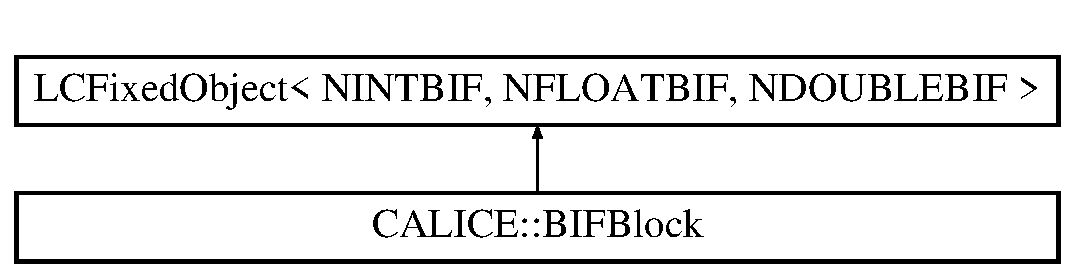
\includegraphics[height=2.000000cm]{classCALICE_1_1BIFBlock}
\end{center}
\end{figure}
\subsection*{Public Member Functions}
\begin{DoxyCompactItemize}
\item 
{\bf B\-I\-F\-Block} ()\label{classCALICE_1_1BIFBlock_a07e68d7015e5012ce8d2c6fcff0cb1ba}

\begin{DoxyCompactList}\small\item\em Constructor. \end{DoxyCompactList}\item 
{\bfseries B\-I\-F\-Block} (L\-C\-Object $\ast$obj)\label{classCALICE_1_1BIFBlock_a90292dce08c6dfe322f7491ba923faf8}

\item 
{\bf B\-I\-F\-Block} (int Trigger\-Source, int B\-X\-I\-D\-\_\-\-B\-I\-F, float Time\-\_\-\-B\-I\-F, int B\-I\-F\-\_\-\-Offset=0)\label{classCALICE_1_1BIFBlock_ab7433bcd66f140c004d4f8eefb2f9055}

\begin{DoxyCompactList}\small\item\em Convenient constructor. \end{DoxyCompactList}\item 
virtual {\bf $\sim$\-B\-I\-F\-Block} ()\label{classCALICE_1_1BIFBlock_a66d7f8a31626549b3c7b1b117cf70ae1}

\begin{DoxyCompactList}\small\item\em Destructor. \end{DoxyCompactList}\item 
void {\bf print} (std\-::ostream \&os, int)\label{classCALICE_1_1BIFBlock_a95fa0c06efa6a87da8cf1e8380072cde}

\begin{DoxyCompactList}\small\item\em Convenient print method. \end{DoxyCompactList}\item 
void {\bf set\-Trigger\-Source} (int Trigger\-Source)\label{classCALICE_1_1BIFBlock_a011c8771a288f584e02335821ecd2aa9}

\begin{DoxyCompactList}\small\item\em Set Trigger type. \end{DoxyCompactList}\item 
void {\bf set\-B\-X\-I\-D} (int B\-X\-I\-D\-\_\-\-B\-I\-F)\label{classCALICE_1_1BIFBlock_a089b2f4c9b362e0f95e8942f559bdfcd}

\begin{DoxyCompactList}\small\item\em Set B\-X\-I\-D of the B\-I\-F Trigger. \end{DoxyCompactList}\item 
void {\bf set\-Offset} (int B\-I\-F\-\_\-\-Offset)\label{classCALICE_1_1BIFBlock_afed1536822bb3c10b959f2e467220f6c}

\begin{DoxyCompactList}\small\item\em Set Time Offset of the B\-I\-F. \end{DoxyCompactList}\item 
void {\bf set\-Time} (float Time\-\_\-\-B\-I\-F)\label{classCALICE_1_1BIFBlock_aa7286d6fe67c4c941537a0f156812247}

\begin{DoxyCompactList}\small\item\em Set Time of the B\-I\-F Trigger. \end{DoxyCompactList}\item 
const int {\bf get\-Trigger\-Source} () const \label{classCALICE_1_1BIFBlock_a27cde06f0406d3908efc8ec0b047332e}

\begin{DoxyCompactList}\small\item\em Get Trigger type. \end{DoxyCompactList}\item 
const int {\bf get\-B\-X\-I\-D} () const \label{classCALICE_1_1BIFBlock_a7104742c4a7d0a3a17b0e195371ccf4c}

\begin{DoxyCompactList}\small\item\em Get B\-X\-I\-D of the B\-I\-F Trigger. \end{DoxyCompactList}\item 
const int {\bf get\-Offset} () const \label{classCALICE_1_1BIFBlock_ab1c2e7d77b59f9725db51ed27bc74312}

\begin{DoxyCompactList}\small\item\em Get Time Offset of the B\-I\-F. \end{DoxyCompactList}\item 
const float {\bf get\-Time} () const \label{classCALICE_1_1BIFBlock_a78df0b79c7631dd015db810eb5e653cd}

\begin{DoxyCompactList}\small\item\em Get Time of the B\-I\-F Trigger. \end{DoxyCompactList}\item 
const std\-::string {\bf get\-Type\-Name} () const \label{classCALICE_1_1BIFBlock_afedd9050ce2f4ae465c0c5c69ace43e9}

\begin{DoxyCompactList}\small\item\em Return the type of the class. \end{DoxyCompactList}\item 
const std\-::string {\bf get\-Data\-Description} () const \label{classCALICE_1_1BIFBlock_a103f8aa8e9bc3073acfd2adb865342f0}

\begin{DoxyCompactList}\small\item\em Return a brief description of the data members. \end{DoxyCompactList}\end{DoxyCompactItemize}


\subsection{Detailed Description}
Class for the S\-L\-C\-I\-O E\-U\-D\-A\-Q B\-I\-F Data as acquired by the E\-U\-D\-A\-Q system. 

\begin{DoxyAuthor}{Author}
E.\-Brianne @ D\-E\-S\-Y Hamburg 
\end{DoxyAuthor}
\begin{DoxyDate}{Date}
May 2016 Created for 2016 testbeams E\-U\-D\-A\-Q data format. 
\end{DoxyDate}


Definition at line 37 of file B\-I\-F\-Block.\-hh.



The documentation for this class was generated from the following file\-:\begin{DoxyCompactItemize}
\item 
B\-I\-F\-Block.\-hh\end{DoxyCompactItemize}

\section{C\-A\-L\-I\-C\-E\-:\-:D\-W\-C\-Block Class Reference}
\label{classCALICE_1_1DWCBlock}\index{C\-A\-L\-I\-C\-E\-::\-D\-W\-C\-Block@{C\-A\-L\-I\-C\-E\-::\-D\-W\-C\-Block}}


Class for the D\-W\-C track information.  




{\ttfamily \#include $<$D\-W\-C\-Block.\-hh$>$}

Inheritance diagram for C\-A\-L\-I\-C\-E\-:\-:D\-W\-C\-Block\-:\begin{figure}[H]
\begin{center}
\leavevmode
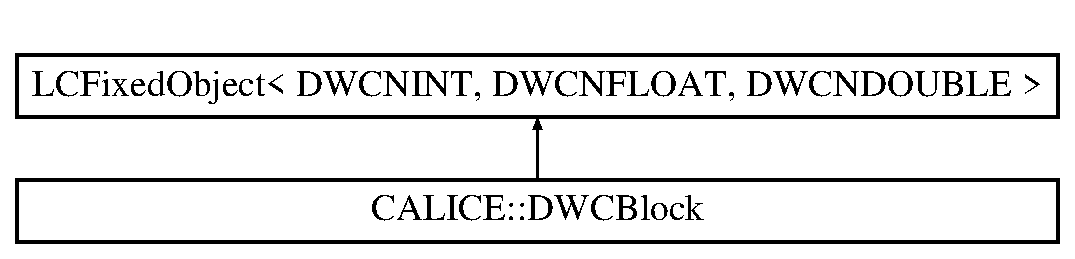
\includegraphics[height=2.000000cm]{classCALICE_1_1DWCBlock}
\end{center}
\end{figure}
\subsection*{Public Member Functions}
\begin{DoxyCompactItemize}
\item 
{\bf D\-W\-C\-Block} ()\label{classCALICE_1_1DWCBlock_a23f02464f283721d4993cff8cd5c8eef}

\begin{DoxyCompactList}\small\item\em Constructor. \end{DoxyCompactList}\item 
{\bfseries D\-W\-C\-Block} (L\-C\-Object $\ast$obj)\label{classCALICE_1_1DWCBlock_ab878aed4b01d1caf9ebeeec343bfa062}

\item 
{\bf D\-W\-C\-Block} (float segment\-X, float segment\-Y, float slope\-X, float slope\-Y)\label{classCALICE_1_1DWCBlock_af604f480f1847f1558ab7cac1027e942}

\begin{DoxyCompactList}\small\item\em Convenient constructor. \end{DoxyCompactList}\item 
virtual {\bf $\sim$\-D\-W\-C\-Block} ()\label{classCALICE_1_1DWCBlock_a69a20263fd7a3eb28dc65f2a1759047a}

\begin{DoxyCompactList}\small\item\em Destructor. \end{DoxyCompactList}\item 
void {\bf print} (std\-::ostream \&os, int)\label{classCALICE_1_1DWCBlock_a90acbeb3f3d2a8eae72177784bf13deb}

\begin{DoxyCompactList}\small\item\em Convenient print method. \end{DoxyCompactList}\item 
void {\bf set\-Segment\-X} (int segment\-X)\label{classCALICE_1_1DWCBlock_a9eaaba8d0e2acd92bc849fd7a4a17f34}

\begin{DoxyCompactList}\small\item\em Set Segments. \end{DoxyCompactList}\item 
void {\bfseries set\-Segment\-Y} (int segment\-Y)\label{classCALICE_1_1DWCBlock_ae64f6788fa1e258e06eda8941a9a6689}

\item 
void {\bf set\-Slope\-X} (int slope\-X)\label{classCALICE_1_1DWCBlock_afcbe9b073eb3d80d15e6ceb6aad33f83}

\begin{DoxyCompactList}\small\item\em Set Slopes. \end{DoxyCompactList}\item 
void {\bfseries set\-Slope\-Y} (int slope\-Y)\label{classCALICE_1_1DWCBlock_a22f058df6f5d6979bf499a92cc3de5c7}

\item 
const float {\bf get\-Segment\-X} () const \label{classCALICE_1_1DWCBlock_acfb4a3ed04d0fdf80eb86db4e7371c58}

\begin{DoxyCompactList}\small\item\em Get Segments of the Track. \end{DoxyCompactList}\item 
const float {\bfseries get\-Segment\-Y} () const \label{classCALICE_1_1DWCBlock_a9a9204de822bef1302c3dc972e77da50}

\item 
const float {\bf get\-Slope\-X} () const \label{classCALICE_1_1DWCBlock_af108c3b0f57fe894907b785e2c3a99eb}

\begin{DoxyCompactList}\small\item\em Get Slopes of the Track. \end{DoxyCompactList}\item 
const float {\bfseries get\-Slope\-Y} () const \label{classCALICE_1_1DWCBlock_ad4d68ef2dbf95df38f0aef8f27bcd65c}

\item 
const std\-::string {\bf get\-Type\-Name} () const \label{classCALICE_1_1DWCBlock_acccf76b379873f8b81e26c9974cd6381}

\begin{DoxyCompactList}\small\item\em Return the type of the class. \end{DoxyCompactList}\item 
const std\-::string {\bf get\-Data\-Description} () const \label{classCALICE_1_1DWCBlock_a48a3047dfef2c94b1124b0c908c44995}

\begin{DoxyCompactList}\small\item\em Return a brief description of the data members. \end{DoxyCompactList}\end{DoxyCompactItemize}


\subsection{Detailed Description}
Class for the D\-W\-C track information. 

\begin{DoxyAuthor}{Author}
L.\-Linghui @ University of Tokyo 
\end{DoxyAuthor}
\begin{DoxyDate}{Date}
Aug. 2018 Created for 2018 testbeams D\-W\-C 
\end{DoxyDate}


Definition at line 24 of file D\-W\-C\-Block.\-hh.



The documentation for this class was generated from the following file\-:\begin{DoxyCompactItemize}
\item 
D\-W\-C\-Block.\-hh\end{DoxyCompactItemize}

\section{C\-A\-L\-I\-C\-E\-:\-:D\-W\-C\-Processor Class Reference}
\label{classCALICE_1_1DWCProcessor}\index{C\-A\-L\-I\-C\-E\-::\-D\-W\-C\-Processor@{C\-A\-L\-I\-C\-E\-::\-D\-W\-C\-Processor}}
Inheritance diagram for C\-A\-L\-I\-C\-E\-:\-:D\-W\-C\-Processor\-:\begin{figure}[H]
\begin{center}
\leavevmode
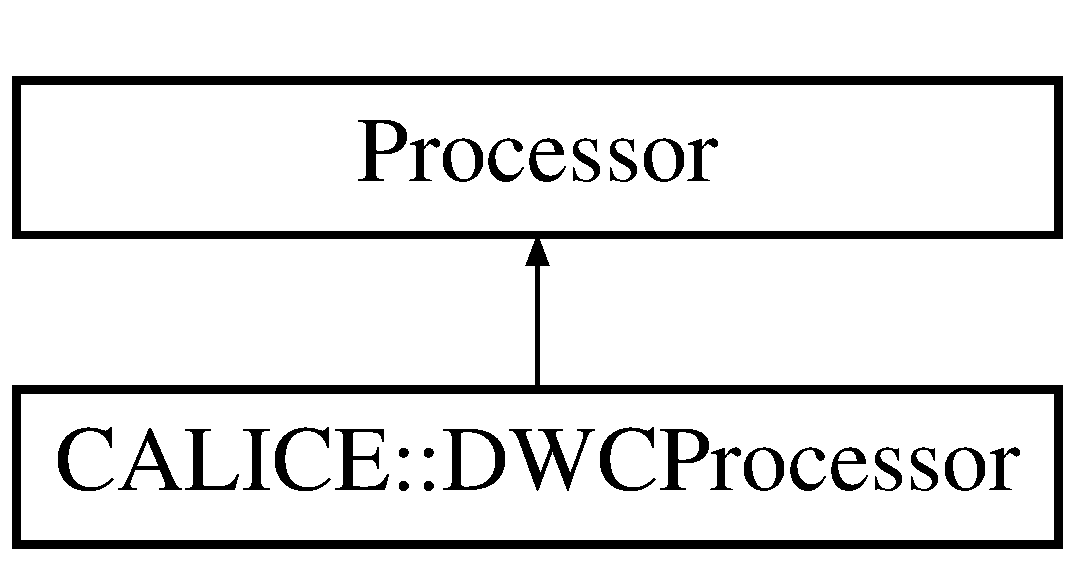
\includegraphics[height=2.000000cm]{classCALICE_1_1DWCProcessor}
\end{center}
\end{figure}
\subsection*{Public Member Functions}
\begin{DoxyCompactItemize}
\item 
virtual Processor $\ast$ {\bf new\-Processor} ()\label{classCALICE_1_1DWCProcessor_a007fa240c5beafc5364c733741f6a51f}

\begin{DoxyCompactList}\small\item\em Implementation of new Processor returns pointer to processor. \end{DoxyCompactList}\item 
void {\bf process\-Event} (L\-C\-Event $\ast$evt)\label{classCALICE_1_1DWCProcessor_a383de0f47632539b18b913c65cdc965e}

\begin{DoxyCompactList}\small\item\em Creates events with L\-C\-Genreal\-Object collections from the E\-U\-D\-A\-Q input file and calls all active processors' \doxyref{process\-Event()}{p.}{classCALICE_1_1DWCProcessor_a383de0f47632539b18b913c65cdc965e} and process\-Run\-Header Method. \end{DoxyCompactList}\item 
virtual void {\bf init} ()\label{classCALICE_1_1DWCProcessor_ad557578e5f28eaf5e48cb9af448d5d7c}

\begin{DoxyCompactList}\small\item\em init method \end{DoxyCompactList}\item 
virtual void {\bf end} ()\label{classCALICE_1_1DWCProcessor_a7403f807486b02347011baa13020cbbd}

\begin{DoxyCompactList}\small\item\em end method \end{DoxyCompactList}\item 
virtual void {\bfseries print\-Parameters} ()\label{classCALICE_1_1DWCProcessor_a7605fb778019459e4560b23e4767ab08}

\end{DoxyCompactItemize}
\subsection*{Protected Types}
\begin{DoxyCompactItemize}
\item 
enum {\bfseries D\-W\-C\-\_\-\-M\-A\-P} \{ {\bfseries D\-W\-C\-\_\-\-A}, 
{\bfseries D\-W\-C\-\_\-\-D}, 
{\bfseries D\-W\-C\-\_\-\-E}, 
{\bfseries D\-W\-C\-\_\-\-E\-X\-T}
 \}
\item 
enum {\bfseries D\-W\-C\-\_\-to\-\_\-\-T\-D\-C\-\_\-\-M\-A\-P} \{ \\*
{\bfseries D\-W\-C\-E\-\_\-\-L} = 0, 
{\bfseries D\-W\-C\-E\-\_\-\-R} = 1, 
{\bfseries D\-W\-C\-E\-\_\-\-D} = 2, 
{\bfseries D\-W\-C\-E\-\_\-\-U} = 3, 
\\*
{\bfseries D\-W\-C\-D\-\_\-\-L} = 4, 
{\bfseries D\-W\-C\-D\-\_\-\-R} = 5, 
{\bfseries D\-W\-C\-D\-\_\-\-D} = 6, 
{\bfseries D\-W\-C\-D\-\_\-\-U} = 7, 
\\*
{\bfseries D\-W\-C\-A\-\_\-\-L} = 9, 
{\bfseries D\-W\-C\-A\-\_\-\-R} = 8, 
{\bfseries D\-W\-C\-A\-\_\-\-D} = 10, 
{\bfseries D\-W\-C\-A\-\_\-\-U} = 11, 
\\*
{\bfseries D\-W\-C\-E\-X\-T\-\_\-\-L} = 13, 
{\bfseries D\-W\-C\-E\-X\-T\-\_\-\-R} = 12, 
{\bfseries D\-W\-C\-E\-X\-T\-\_\-\-D} = 14, 
{\bfseries D\-W\-C\-E\-X\-T\-\_\-\-U} = 15
 \}
\end{DoxyCompactItemize}
\subsection*{Protected Member Functions}
\begin{DoxyCompactItemize}
\item 
int {\bfseries load\-\_\-ahcal\-\_\-tdc} ()\label{classCALICE_1_1DWCProcessor_a8dc7ad6a9a383394675edd702759b051}

\item 
int {\bfseries load\-\_\-bif\-\_\-tdc} ()\label{classCALICE_1_1DWCProcessor_ad321c9c914af0d5bf51e3e536e65bdbe}

\item 
void {\bfseries event\-\_\-match} ()\label{classCALICE_1_1DWCProcessor_aee60b0b2be239ee0404c4f7cd0118bbc}

\end{DoxyCompactItemize}
\subsection*{Protected Attributes}
\begin{DoxyCompactItemize}
\item 
std\-::string {\bfseries \-\_\-input\-Col\-Name\-B\-I\-F}\label{classCALICE_1_1DWCProcessor_a017895c81a7349f917fab51a4e07c452}

\item 
std\-::string {\bfseries \-\_\-input\-File\-Name\-B\-I\-F}\label{classCALICE_1_1DWCProcessor_ab1502aaac0fd11abdd5c0c9b45259828}

\item 
std\-::string {\bfseries \-\_\-input\-File\-Name\-A\-H\-C\-A\-L}\label{classCALICE_1_1DWCProcessor_a674b7122596328f711d2e7c3844e1e07}

\item 
std\-::string {\bfseries \-\_\-input\-File\-Name\-D\-W\-C}\label{classCALICE_1_1DWCProcessor_a8f4eeca5ae42f2f40cfed3e75f05ce5d}

\item 
F\-I\-L\-E $\ast$ {\bfseries \-\_\-bif\-File}\label{classCALICE_1_1DWCProcessor_aabc149e980830e73711862fa353b458e}

\item 
F\-I\-L\-E $\ast$ {\bfseries \-\_\-ahcal\-File}\label{classCALICE_1_1DWCProcessor_a0d7e6e58f9b4f124f70337b83c4442af}

\item 
T\-File $\ast$ {\bfseries \-\_\-dwc\-File}\label{classCALICE_1_1DWCProcessor_a5b445b5c73a2a91b34766b6732528636}

\item 
T\-Tree $\ast$ {\bfseries \-\_\-dwc\-Tree}\label{classCALICE_1_1DWCProcessor_a1a2c2ad7e7b675b40e9f0e04ee9b6554}

\item 
std\-::string {\bfseries \-\_\-output\-Col\-Name\-D\-W\-C}\label{classCALICE_1_1DWCProcessor_a69b8d3123d50eaa2cd54ad23eaf91219}

\item 
unsigned long long int {\bfseries \-\_\-\-B\-I\-F\-T\-D\-C}\label{classCALICE_1_1DWCProcessor_ae4eef30649f5df4cf4d20a48dafc3c0c}

\item 
unsigned long long int {\bfseries \-\_\-\-A\-H\-C\-A\-L\-T\-D\-C}\label{classCALICE_1_1DWCProcessor_a75b49d844b2c3c7d050a25f55106d4dd}

\item 
std\-::vector$<$ unsigned long \\*
long int $>$ {\bfseries \-\_\-\-B\-I\-F\-Time}\label{classCALICE_1_1DWCProcessor_ab466420698f295ef21a5db885a5dcd68}

\item 
std\-::vector$<$ unsigned long \\*
long int $>$ {\bfseries \-\_\-\-D\-W\-C\-Time}\label{classCALICE_1_1DWCProcessor_a379f7ecee4966b7ab72530674b6ee674}

\item 
std\-::vector$<$ unsigned int $>$ {\bfseries \-\_\-\-D\-W\-C\-Trig}\label{classCALICE_1_1DWCProcessor_a29b4425aebc414dd4a1edf8519ff0175}

\item 
unsigned int {\bfseries \-\_\-index}\label{classCALICE_1_1DWCProcessor_a6a714884b6fbaf24742bb495a39c5d33}

\item 
std\-::vector$<$ int $>$ $\ast$ {\bfseries \-\_\-dwc\-Ch} [16] = \{0\}\label{classCALICE_1_1DWCProcessor_ad13b2866ef4bfb0453a8eabd26127a3c}

\item 
const int {\bfseries B\-U\-N\-C\-H\-\_\-\-T\-H\-R} = 5000\label{classCALICE_1_1DWCProcessor_ad554556b8dd863f01c86df433f1fdfda}

\item 
const int {\bfseries D\-W\-C\-\_\-\-T\-H\-R} = 4\label{classCALICE_1_1DWCProcessor_ae85ac22f0b1703dc6399a0b41a6edc22}

\item 
{\bf Line\-Fitter} {\bfseries \-\_\-track\-X}\label{classCALICE_1_1DWCProcessor_adafcec7c2d188557f96e50935aefe870}

\item 
{\bf Line\-Fitter} {\bfseries \-\_\-track\-Y}\label{classCALICE_1_1DWCProcessor_a307d2494f7fcc7fd07f2803f34af24ea}

\item 
\begin{tabbing}
xx\=xx\=xx\=xx\=xx\=xx\=xx\=xx\=xx\=\kill
struct \{\\
\>float {\bfseries A\_X} = -\/1.29\\
\>float {\bfseries A\_Y} = -\/2.54\\
\>float {\bfseries D\_X} = -\/0.56\\
\>float {\bfseries D\_Y} = -\/7.36\\
\>float {\bfseries E\_X} = -\/2.20\\
\>float {\bfseries E\_Y} = -\/7.49\\
\} {\bfseries DWC\_Offset}\label{classCALICE_1_1DWCProcessor_a385dce0ff2577432d1613a8a86e44565}
\\

\end{tabbing}\item 
std\-::vector$<$ float $>$ {\bfseries \-\_\-\-D\-W\-C\-Offsets}\label{classCALICE_1_1DWCProcessor_a0621e94d17c76d9059c4078740243491}

\item 
const float {\bfseries D\-W\-C\-\_\-\-Z\-\_\-\-E} = -\/1090\label{classCALICE_1_1DWCProcessor_a64d00114aa1fc76520d822093aad047f}

\item 
const float {\bfseries D\-W\-C\-\_\-\-Z\-\_\-\-D} = -\/2350\label{classCALICE_1_1DWCProcessor_a183b71d4e9de86f78584fa89f2af7a0d}

\item 
const float {\bfseries D\-W\-C\-\_\-\-Z\-\_\-\-A} = -\/15090\label{classCALICE_1_1DWCProcessor_a281ba3794ef5a9f91a510a60d41616ff}

\item 
const float {\bfseries D\-W\-C\-\_\-\-Z\-\_\-\-E\-X\-T} = -\/17690\label{classCALICE_1_1DWCProcessor_a1eca5dc962b741bf8a9a98a0a6736c22}

\end{DoxyCompactItemize}


\subsection{Detailed Description}


Definition at line 24 of file D\-W\-C\-Processor.\-hh.



The documentation for this class was generated from the following files\-:\begin{DoxyCompactItemize}
\item 
D\-W\-C\-Processor.\-hh\item 
D\-W\-C\-Processor.\-cc\end{DoxyCompactItemize}

\section{C\-A\-L\-I\-C\-E\-:\-:E\-U\-D\-A\-Q\-Block Class Reference}
\label{classCALICE_1_1EUDAQBlock}\index{C\-A\-L\-I\-C\-E\-::\-E\-U\-D\-A\-Q\-Block@{C\-A\-L\-I\-C\-E\-::\-E\-U\-D\-A\-Q\-Block}}


Class for the S\-L\-C\-I\-O E\-U\-D\-A\-Q Data as acquired by the E\-U\-D\-A\-Q system.  




{\ttfamily \#include $<$E\-U\-D\-A\-Q\-Block.\-hh$>$}

Inheritance diagram for C\-A\-L\-I\-C\-E\-:\-:E\-U\-D\-A\-Q\-Block\-:\begin{figure}[H]
\begin{center}
\leavevmode
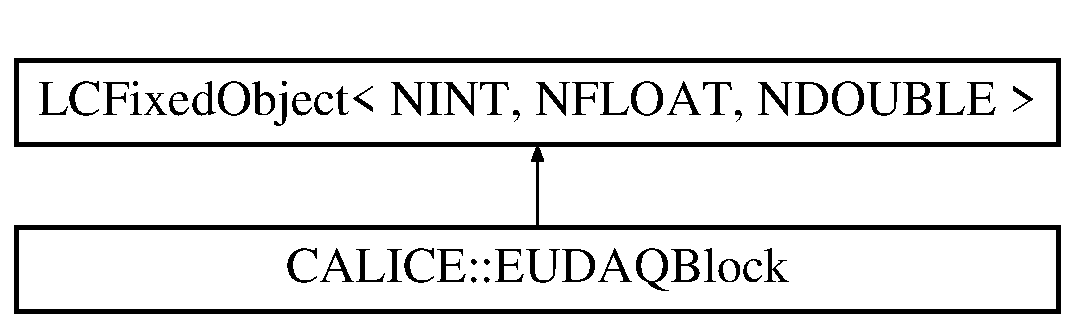
\includegraphics[height=2.000000cm]{classCALICE_1_1EUDAQBlock}
\end{center}
\end{figure}
\subsection*{Public Member Functions}
\begin{DoxyCompactItemize}
\item 
{\bf E\-U\-D\-A\-Q\-Block} (int Cycle\-Nr, int Bunch\-X\-I\-D, int Chip\-I\-D, int Evt\-Nr, int Channel, int T\-D\-C, int A\-D\-C, int Hit\-Bit, int Gain\-Bit)\label{classCALICE_1_1EUDAQBlock_a2576c4ead40588d8ea075d9629926ce3}

\begin{DoxyCompactList}\small\item\em Convenient c'tor. \end{DoxyCompactList}\item 
{\bf E\-U\-D\-A\-Q\-Block} (L\-C\-Object $\ast$obj)\label{classCALICE_1_1EUDAQBlock_adf2c1a0b660a881f637ae260033b2068}

\begin{DoxyCompactList}\small\item\em 'Copy constructor' needed to interpret L\-C\-Collection read from file/database. \end{DoxyCompactList}\item 
virtual {\bf $\sim$\-E\-U\-D\-A\-Q\-Block} ()\label{classCALICE_1_1EUDAQBlock_ac009640c79883d5b236ffa1f01a4da08}

\begin{DoxyCompactList}\small\item\em Important for memory handling. \end{DoxyCompactList}\item 
int {\bf Get\-Cycle\-Nr} () const \label{classCALICE_1_1EUDAQBlock_a7267f8e75e5ee64c2b558a1cb58b5370}

\begin{DoxyCompactList}\small\item\em get the Cycle\-Nr. \end{DoxyCompactList}\item 
int {\bf Get\-Bunch\-X\-I\-D} () const \label{classCALICE_1_1EUDAQBlock_a9e868629e66c71f4a5086ee4515d75a6}

\begin{DoxyCompactList}\small\item\em get the Bunch\-X\-I\-D. \end{DoxyCompactList}\item 
int {\bf Get\-Chip\-I\-D} () const \label{classCALICE_1_1EUDAQBlock_a29e7cb6cea36a5726c185af80f602a04}

\begin{DoxyCompactList}\small\item\em get the Chip\-I\-D. \end{DoxyCompactList}\item 
int {\bf Get\-Evt\-Nr} () const \label{classCALICE_1_1EUDAQBlock_a274bfd6d90f473f1875fd2045268e27f}

\begin{DoxyCompactList}\small\item\em get the Evt\-Nr. \end{DoxyCompactList}\item 
int {\bf Get\-Channel} () const \label{classCALICE_1_1EUDAQBlock_a5665cd40d1deb96c634a7e131be981a8}

\begin{DoxyCompactList}\small\item\em get the Channel. \end{DoxyCompactList}\item 
int {\bf Get\-T\-D\-C} () const \label{classCALICE_1_1EUDAQBlock_a66a6c244efdc2357b15350e778f98e56}

\begin{DoxyCompactList}\small\item\em get the T\-D\-C. \end{DoxyCompactList}\item 
int {\bf Get\-A\-D\-C} () const \label{classCALICE_1_1EUDAQBlock_ac6ad7fd2adcc72ed2aa861eac4d89a0d}

\begin{DoxyCompactList}\small\item\em get the A\-D\-C. \end{DoxyCompactList}\item 
int {\bf Get\-Hit\-Bit} () const \label{classCALICE_1_1EUDAQBlock_a42be25f91cc050d64bba79ff4718b5c4}

\begin{DoxyCompactList}\small\item\em get the Hit\-Bit. \end{DoxyCompactList}\item 
int {\bf Get\-Gain\-Bit} () const \label{classCALICE_1_1EUDAQBlock_ac2573362003677a183343529bc63d74c}

\begin{DoxyCompactList}\small\item\em get the Gain\-Bit. \end{DoxyCompactList}\item 
void {\bf print} (std\-::ostream \&os, int)\label{classCALICE_1_1EUDAQBlock_a4f65b14367aa1123dd7a8a74e5d24ee1}

\begin{DoxyCompactList}\small\item\em Convenient print method. \end{DoxyCompactList}\item 
const std\-::string {\bf get\-Type\-Name} () const \label{classCALICE_1_1EUDAQBlock_aea8613f7fc6cbb4bcbc0294a020d3eca}

\begin{DoxyCompactList}\small\item\em Return the type of the class. \end{DoxyCompactList}\item 
const std\-::string {\bf get\-Data\-Description} () const \label{classCALICE_1_1EUDAQBlock_a48d80a041501c9eaada74c500d78074c}

\begin{DoxyCompactList}\small\item\em Return a brief description of the data members. \end{DoxyCompactList}\end{DoxyCompactItemize}


\subsection{Detailed Description}
Class for the S\-L\-C\-I\-O E\-U\-D\-A\-Q Data as acquired by the E\-U\-D\-A\-Q system. 

\begin{DoxyAuthor}{Author}
A. Irles, based on the \doxyref{Labview\-Block2}{p.}{classCALICE_1_1LabviewBlock2} writen by S. Lu D\-E\-S\-Y Hamburg 
\end{DoxyAuthor}
\begin{DoxyDate}{Date}
May 20 2015 Created for 2015 testbeams E\-U\-D\-A\-Q data format. 
\end{DoxyDate}


Definition at line 23 of file E\-U\-D\-A\-Q\-Block.\-hh.



The documentation for this class was generated from the following file\-:\begin{DoxyCompactItemize}
\item 
E\-U\-D\-A\-Q\-Block.\-hh\end{DoxyCompactItemize}

\section{C\-A\-L\-I\-C\-E\-:\-:E\-U\-D\-A\-Q\-Block2016 Class Reference}
\label{classCALICE_1_1EUDAQBlock2016}\index{C\-A\-L\-I\-C\-E\-::\-E\-U\-D\-A\-Q\-Block2016@{C\-A\-L\-I\-C\-E\-::\-E\-U\-D\-A\-Q\-Block2016}}


Class for the S\-L\-C\-I\-O E\-U\-D\-A\-Q Data as acquired by the E\-U\-D\-A\-Q system.  




{\ttfamily \#include $<$E\-U\-D\-A\-Q\-Block2016.\-hh$>$}

Inheritance diagram for C\-A\-L\-I\-C\-E\-:\-:E\-U\-D\-A\-Q\-Block2016\-:\begin{figure}[H]
\begin{center}
\leavevmode
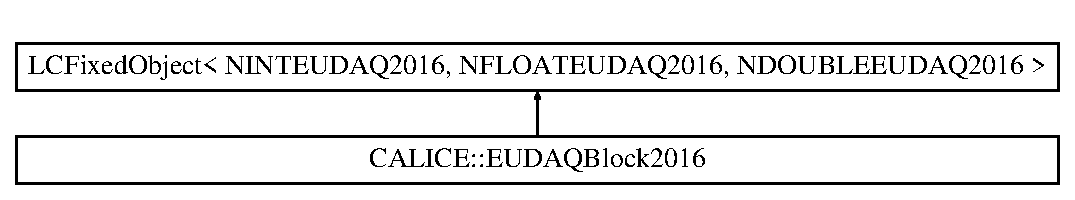
\includegraphics[height=2.000000cm]{classCALICE_1_1EUDAQBlock2016}
\end{center}
\end{figure}
\subsection*{Public Member Functions}
\begin{DoxyCompactItemize}
\item 
{\bf E\-U\-D\-A\-Q\-Block2016} (int Cycle\-Nr, int Bunch\-X\-I\-D, int Evt\-Nr, int Chip\-I\-D, int N\-Channels, int T\-D\-C\-\_\-0, int T\-D\-C\-\_\-1, int T\-D\-C\-\_\-2, int T\-D\-C\-\_\-3, int T\-D\-C\-\_\-4, int T\-D\-C\-\_\-5, int T\-D\-C\-\_\-6, int T\-D\-C\-\_\-7, int T\-D\-C\-\_\-8, int T\-D\-C\-\_\-9, int T\-D\-C\-\_\-10, int T\-D\-C\-\_\-11, int T\-D\-C\-\_\-12, int T\-D\-C\-\_\-13, int T\-D\-C\-\_\-14, int T\-D\-C\-\_\-15, int T\-D\-C\-\_\-16, int T\-D\-C\-\_\-17, int T\-D\-C\-\_\-18, int T\-D\-C\-\_\-19, int T\-D\-C\-\_\-20, int T\-D\-C\-\_\-21, int T\-D\-C\-\_\-22, int T\-D\-C\-\_\-23, int T\-D\-C\-\_\-24, int T\-D\-C\-\_\-25, int T\-D\-C\-\_\-26, int T\-D\-C\-\_\-27, int T\-D\-C\-\_\-28, int T\-D\-C\-\_\-29, int T\-D\-C\-\_\-30, int T\-D\-C\-\_\-31, int T\-D\-C\-\_\-32, int T\-D\-C\-\_\-33, int T\-D\-C\-\_\-34, int T\-D\-C\-\_\-35, int A\-D\-C\-\_\-0, int A\-D\-C\-\_\-1, int A\-D\-C\-\_\-2, int A\-D\-C\-\_\-3, int A\-D\-C\-\_\-4, int A\-D\-C\-\_\-5, int A\-D\-C\-\_\-6, int A\-D\-C\-\_\-7, int A\-D\-C\-\_\-8, int A\-D\-C\-\_\-9, int A\-D\-C\-\_\-10, int A\-D\-C\-\_\-11, int A\-D\-C\-\_\-12, int A\-D\-C\-\_\-13, int A\-D\-C\-\_\-14, int A\-D\-C\-\_\-15, int A\-D\-C\-\_\-16, int A\-D\-C\-\_\-17, int A\-D\-C\-\_\-18, int A\-D\-C\-\_\-19, int A\-D\-C\-\_\-20, int A\-D\-C\-\_\-21, int A\-D\-C\-\_\-22, int A\-D\-C\-\_\-23, int A\-D\-C\-\_\-24, int A\-D\-C\-\_\-25, int A\-D\-C\-\_\-26, int A\-D\-C\-\_\-27, int A\-D\-C\-\_\-28, int A\-D\-C\-\_\-29, int A\-D\-C\-\_\-30, int A\-D\-C\-\_\-31, int A\-D\-C\-\_\-32, int A\-D\-C\-\_\-33, int A\-D\-C\-\_\-34, int A\-D\-C\-\_\-35)\label{classCALICE_1_1EUDAQBlock2016_a695944edb5478e333e57bdf36b550cfe}

\begin{DoxyCompactList}\small\item\em Very ugly constructor because we use a Generic Object with many integers. \end{DoxyCompactList}\item 
{\bf E\-U\-D\-A\-Q\-Block2016} (L\-C\-Object $\ast$obj)\label{classCALICE_1_1EUDAQBlock2016_a69846d216e879d4d09388d712444ed6f}

\begin{DoxyCompactList}\small\item\em 'Copy constructor' needed to interpret L\-C\-Collection read from file/database. \end{DoxyCompactList}\item 
virtual {\bf $\sim$\-E\-U\-D\-A\-Q\-Block2016} ()\label{classCALICE_1_1EUDAQBlock2016_af60b7d8dbc353c11a2cb10767bd686fa}

\begin{DoxyCompactList}\small\item\em Important for memory handling. \end{DoxyCompactList}\item 
int {\bf Get\-Cycle\-Nr} () const \label{classCALICE_1_1EUDAQBlock2016_a2250dc2f09ed14a48ef46c97778cf0a5}

\begin{DoxyCompactList}\small\item\em get the Cycle\-Nr. \end{DoxyCompactList}\item 
int {\bf Get\-Bunch\-X\-I\-D} () const \label{classCALICE_1_1EUDAQBlock2016_ad255cb104666592cf7910092bfaa4283}

\begin{DoxyCompactList}\small\item\em get the Bunch\-X\-I\-D. \end{DoxyCompactList}\item 
int {\bf Get\-Evt\-Nr} () const \label{classCALICE_1_1EUDAQBlock2016_a7d950b9ed9fd1e3a75d511410b236218}

\begin{DoxyCompactList}\small\item\em get the Evt\-Nr. \end{DoxyCompactList}\item 
int {\bf Get\-Chip\-I\-D} () const \label{classCALICE_1_1EUDAQBlock2016_ab93d2b651d880a6a2d7dd0f5e258b3e9}

\begin{DoxyCompactList}\small\item\em get the Chip\-I\-D. \end{DoxyCompactList}\item 
int {\bf Get\-N\-Channels} () const \label{classCALICE_1_1EUDAQBlock2016_a0a292a54aeb98815e03589dc159615bf}

\begin{DoxyCompactList}\small\item\em get the Channel. \end{DoxyCompactList}\item 
std\-::vector$<$ int $>$ {\bf Get\-T\-D\-C} () const \label{classCALICE_1_1EUDAQBlock2016_a7889a126a5607b2e316427f24bb7ac5c}

\begin{DoxyCompactList}\small\item\em get the T\-D\-C. \end{DoxyCompactList}\item 
std\-::vector$<$ int $>$ {\bf Get\-A\-D\-C} () const 
\begin{DoxyCompactList}\small\item\em get the Hit\-Bit\-\_\-tdc. \end{DoxyCompactList}\item 
void {\bf print} (std\-::ostream \&os, int)
\begin{DoxyCompactList}\small\item\em get the Hit\-Bit\-\_\-adc. \end{DoxyCompactList}\item 
const std\-::string {\bf get\-Type\-Name} () const \label{classCALICE_1_1EUDAQBlock2016_a0944d67b789f54c706aec430f460dd3a}

\begin{DoxyCompactList}\small\item\em Return the type of the class. \end{DoxyCompactList}\item 
const std\-::string {\bf get\-Data\-Description} () const \label{classCALICE_1_1EUDAQBlock2016_afa918efa6eab716fbcf3ddacd710c8e4}

\begin{DoxyCompactList}\small\item\em Return a brief description of the data members. \end{DoxyCompactList}\end{DoxyCompactItemize}


\subsection{Detailed Description}
Class for the S\-L\-C\-I\-O E\-U\-D\-A\-Q Data as acquired by the E\-U\-D\-A\-Q system. 

\begin{DoxyAuthor}{Author}
A. Irles, based on the \doxyref{E\-U\-D\-A\-Q\-Block}{p.}{classCALICE_1_1EUDAQBlock} writen by A. Irles D\-E\-S\-Y Hamburg 
\end{DoxyAuthor}
\begin{DoxyDate}{Date}
January 12 2016 Created for 2016 testbeams E\-U\-D\-A\-Q data format. 
\end{DoxyDate}


Definition at line 23 of file E\-U\-D\-A\-Q\-Block2016.\-hh.



\subsection{Member Function Documentation}
\index{C\-A\-L\-I\-C\-E\-::\-E\-U\-D\-A\-Q\-Block2016@{C\-A\-L\-I\-C\-E\-::\-E\-U\-D\-A\-Q\-Block2016}!Get\-A\-D\-C@{Get\-A\-D\-C}}
\index{Get\-A\-D\-C@{Get\-A\-D\-C}!CALICE::EUDAQBlock2016@{C\-A\-L\-I\-C\-E\-::\-E\-U\-D\-A\-Q\-Block2016}}
\subsubsection[{Get\-A\-D\-C}]{\setlength{\rightskip}{0pt plus 5cm}std\-::vector$<$int$>$ C\-A\-L\-I\-C\-E\-::\-E\-U\-D\-A\-Q\-Block2016\-::\-Get\-A\-D\-C (
\begin{DoxyParamCaption}
{}
\end{DoxyParamCaption}
) const\hspace{0.3cm}{\ttfamily [inline]}}\label{classCALICE_1_1EUDAQBlock2016_a50fb1b5462489dcb858aa3a5d6f758b9}


get the Hit\-Bit\-\_\-tdc. 

get the Gain\-Bit\-\_\-tdc.\-get the A\-D\-C. 

Definition at line 195 of file E\-U\-D\-A\-Q\-Block2016.\-hh.



Referenced by C\-A\-L\-I\-C\-E\-::\-E\-U\-D\-A\-Q\-Event\-Builder2016\-::process\-Event(), C\-A\-L\-I\-C\-E\-::\-E\-U\-D\-A\-Q\-Event\-Builder2018\-\_\-cosmics\-::process\-Event(), and C\-A\-L\-I\-C\-E\-::\-E\-U\-D\-A\-Q\-Event\-Builder2016\-\_\-wo\-B\-I\-F\-::process\-Event().

\index{C\-A\-L\-I\-C\-E\-::\-E\-U\-D\-A\-Q\-Block2016@{C\-A\-L\-I\-C\-E\-::\-E\-U\-D\-A\-Q\-Block2016}!print@{print}}
\index{print@{print}!CALICE::EUDAQBlock2016@{C\-A\-L\-I\-C\-E\-::\-E\-U\-D\-A\-Q\-Block2016}}
\subsubsection[{print}]{\setlength{\rightskip}{0pt plus 5cm}void C\-A\-L\-I\-C\-E\-::\-E\-U\-D\-A\-Q\-Block2016\-::print (
\begin{DoxyParamCaption}
\item[{std\-::ostream \&}]{os, }
\item[{int}]{}
\end{DoxyParamCaption}
)}\label{classCALICE_1_1EUDAQBlock2016_a9e2a39195b3a46ab7ccccbaaebf0a4a6}


get the Hit\-Bit\-\_\-adc. 

get the Gain\-Bit\-\_\-adc.\-Convenient print method 

The documentation for this class was generated from the following file\-:\begin{DoxyCompactItemize}
\item 
E\-U\-D\-A\-Q\-Block2016.\-hh\end{DoxyCompactItemize}

\section{C\-A\-L\-I\-C\-E\-:\-:E\-U\-D\-A\-Q\-Event\-Builder Class Reference}
\label{classCALICE_1_1EUDAQEventBuilder}\index{C\-A\-L\-I\-C\-E\-::\-E\-U\-D\-A\-Q\-Event\-Builder@{C\-A\-L\-I\-C\-E\-::\-E\-U\-D\-A\-Q\-Event\-Builder}}


Processor for reading the A\-H\-C\-A\-L E\-U\-D\-A\-Q S\-L\-C\-I\-O files.  




{\ttfamily \#include $<$E\-U\-D\-A\-Q\-Event\-Builder.\-hh$>$}

Inheritance diagram for C\-A\-L\-I\-C\-E\-:\-:E\-U\-D\-A\-Q\-Event\-Builder\-:\begin{figure}[H]
\begin{center}
\leavevmode
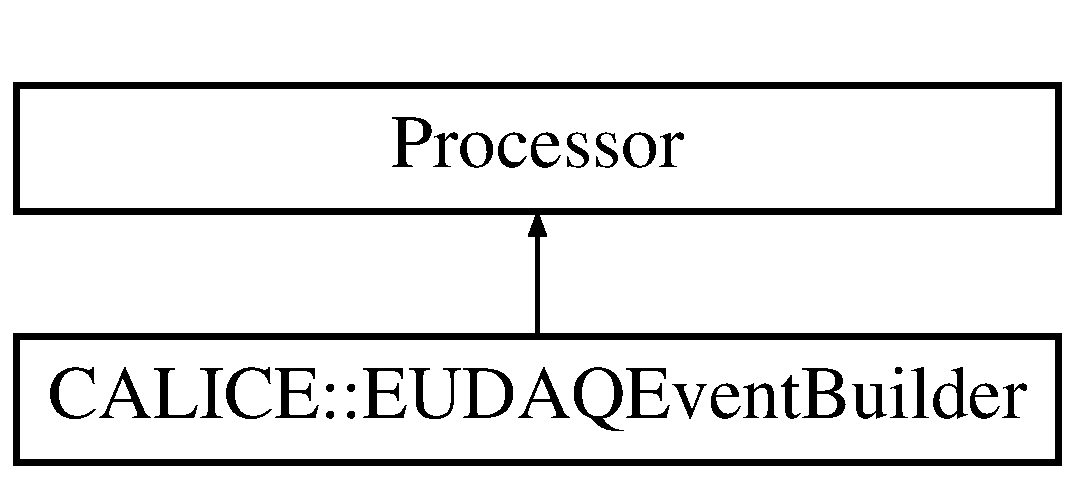
\includegraphics[height=2.000000cm]{classCALICE_1_1EUDAQEventBuilder}
\end{center}
\end{figure}
\subsection*{Data Structures}
\begin{DoxyCompactItemize}
\item 
struct {\bf raw\-Data}
\begin{DoxyCompactList}\small\item\em The slcio data format. \end{DoxyCompactList}\item 
struct {\bf raw\-Temp}
\begin{DoxyCompactList}\small\item\em The slcio data format for the temperature sensor. \end{DoxyCompactList}\end{DoxyCompactItemize}
\subsection*{Public Member Functions}
\begin{DoxyCompactItemize}
\item 
virtual Processor $\ast$ {\bf new\-Processor} ()\label{classCALICE_1_1EUDAQEventBuilder_aa3dc57e6961542850ee8a4690ced210c}

\begin{DoxyCompactList}\small\item\em Implementation of new Processor returns pointer to processor. \end{DoxyCompactList}\item 
void {\bf process\-Event} (L\-C\-Event $\ast$evt)\label{classCALICE_1_1EUDAQEventBuilder_ac54decb0cf83f95f25eeb56e6a68e7a1}

\begin{DoxyCompactList}\small\item\em Creates events with L\-C\-Genreal\-Object collections from the E\-U\-D\-A\-Q input file and calls all active processors' \doxyref{process\-Event()}{p.}{classCALICE_1_1EUDAQEventBuilder_ac54decb0cf83f95f25eeb56e6a68e7a1} and process\-Run\-Header Method. \end{DoxyCompactList}\item 
void {\bf write\-Slow\-Control} ()\label{classCALICE_1_1EUDAQEventBuilder_a0bda9d7aec8ee7ca6ce1c3b8dc6b9795}

\begin{DoxyCompactList}\small\item\em work on slow control data, A\-S\-I\-C \end{DoxyCompactList}\item 
virtual void {\bf init} ()
\begin{DoxyCompactList}\small\item\em work on slow control data, Temperature \end{DoxyCompactList}\item 
virtual void {\bf end} ()\label{classCALICE_1_1EUDAQEventBuilder_a0d15b17c115c16b310055d504ede10a4}

\begin{DoxyCompactList}\small\item\em end method \end{DoxyCompactList}\end{DoxyCompactItemize}
\subsection*{Protected Attributes}
\begin{DoxyCompactItemize}
\item 
std\-::string {\bfseries \-\_\-input\-Col\-Name}\label{classCALICE_1_1EUDAQEventBuilder_af7d60899294e8381b5d81adc95c99ac0}

\item 
std\-::string {\bfseries \-\_\-input\-Col\-Name\-Temp}\label{classCALICE_1_1EUDAQEventBuilder_a2e49295b97dea6c2bdf8edfd95186b7f}

\item 
std\-::string {\bfseries \-\_\-output\-Col\-Name\-E\-C\-A\-L}\label{classCALICE_1_1EUDAQEventBuilder_a1dde63ebdba4c9c0f22c6643f4469aa4}

\item 
std\-::string {\bfseries \-\_\-output\-Col\-Name\-H\-C\-A\-L}\label{classCALICE_1_1EUDAQEventBuilder_ac24b9dbaa1e79ba913d0ed6b74a8b272}

\item 
std\-::string {\bfseries \-\_\-output\-Col\-Name\-Temp}\label{classCALICE_1_1EUDAQEventBuilder_aadd12063b4970b51ed417c88c429ca1c}

\item 
std\-::string {\bfseries \-\_\-detector\-Type\-Name}\label{classCALICE_1_1EUDAQEventBuilder_ae35b525b53a88d398005f79c985c9bca}

\item 
int {\bf \-\_\-run\-Number}\label{classCALICE_1_1EUDAQEventBuilder_a8f4ada65b09422974d99c770bb00307b}

\begin{DoxyCompactList}\small\item\em The run number. \end{DoxyCompactList}\end{DoxyCompactItemize}


\subsection{Detailed Description}
Processor for reading the A\-H\-C\-A\-L E\-U\-D\-A\-Q S\-L\-C\-I\-O files. 

It processes the input data to create events with L\-C\-I\-O collections of the A\-H\-C\-A\-L E\-U\-D\-A\-Q S\-L\-C\-I\-O output (sorted by readout cycles). Based on F. Gaede's Std\-Hep\-Reader to be found in the marlin package. \begin{DoxyAuthor}{Author}
\-: A. Irles (D\-E\-S\-Y), based on the S. Lu's (D\-E\-S\-Y Hamburg) Labview\-Converter2 
\end{DoxyAuthor}
\begin{DoxyDate}{Date}
May 20 2015 
\end{DoxyDate}


Definition at line 22 of file E\-U\-D\-A\-Q\-Event\-Builder.\-hh.



\subsection{Member Function Documentation}
\index{C\-A\-L\-I\-C\-E\-::\-E\-U\-D\-A\-Q\-Event\-Builder@{C\-A\-L\-I\-C\-E\-::\-E\-U\-D\-A\-Q\-Event\-Builder}!init@{init}}
\index{init@{init}!CALICE::EUDAQEventBuilder@{C\-A\-L\-I\-C\-E\-::\-E\-U\-D\-A\-Q\-Event\-Builder}}
\subsubsection[{init}]{\setlength{\rightskip}{0pt plus 5cm}void C\-A\-L\-I\-C\-E\-::\-E\-U\-D\-A\-Q\-Event\-Builder\-::init (
\begin{DoxyParamCaption}
{}
\end{DoxyParamCaption}
)\hspace{0.3cm}{\ttfamily [virtual]}}\label{classCALICE_1_1EUDAQEventBuilder_a7a1f441b5b85da27e467689be7db0a4c}


work on slow control data, Temperature 

init method 

Definition at line 85 of file E\-U\-D\-A\-Q\-Event\-Builder.\-cc.



The documentation for this class was generated from the following files\-:\begin{DoxyCompactItemize}
\item 
E\-U\-D\-A\-Q\-Event\-Builder.\-hh\item 
E\-U\-D\-A\-Q\-Event\-Builder.\-cc\end{DoxyCompactItemize}

\section{C\-A\-L\-I\-C\-E\-:\-:E\-U\-D\-A\-Q\-Event\-Builder2016 Class Reference}
\label{classCALICE_1_1EUDAQEventBuilder2016}\index{C\-A\-L\-I\-C\-E\-::\-E\-U\-D\-A\-Q\-Event\-Builder2016@{C\-A\-L\-I\-C\-E\-::\-E\-U\-D\-A\-Q\-Event\-Builder2016}}


Processor for reading the A\-H\-C\-A\-L E\-U\-D\-A\-Q S\-L\-C\-I\-O files.  




{\ttfamily \#include $<$E\-U\-D\-A\-Q\-Event\-Builder2016.\-hh$>$}

Inheritance diagram for C\-A\-L\-I\-C\-E\-:\-:E\-U\-D\-A\-Q\-Event\-Builder2016\-:\begin{figure}[H]
\begin{center}
\leavevmode
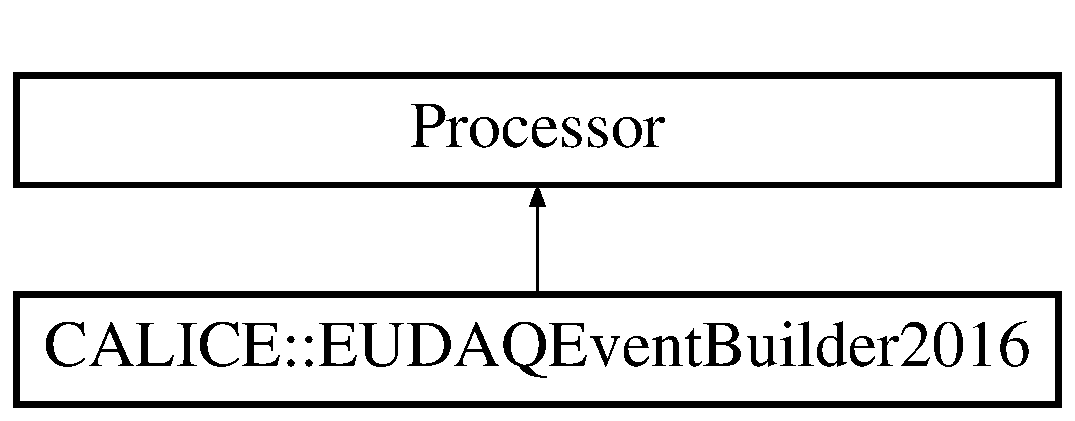
\includegraphics[height=2.000000cm]{classCALICE_1_1EUDAQEventBuilder2016}
\end{center}
\end{figure}
\subsection*{Data Structures}
\begin{DoxyCompactItemize}
\item 
struct {\bf raw\-Data2016}
\begin{DoxyCompactList}\small\item\em The slcio data format. \end{DoxyCompactList}\item 
struct {\bf raw\-Temp}
\begin{DoxyCompactList}\small\item\em The slcio data format for the temperature sensor. \end{DoxyCompactList}\end{DoxyCompactItemize}
\subsection*{Public Member Functions}
\begin{DoxyCompactItemize}
\item 
virtual Processor $\ast$ {\bf new\-Processor} ()\label{classCALICE_1_1EUDAQEventBuilder2016_a1650bf1dce20b0a866b458e9ebdcda7e}

\begin{DoxyCompactList}\small\item\em Implementation of new Processor returns pointer to processor. \end{DoxyCompactList}\item 
void {\bf process\-Event} (L\-C\-Event $\ast$evt)\label{classCALICE_1_1EUDAQEventBuilder2016_a0bac760cc21f4b287c07da49eacc9ada}

\begin{DoxyCompactList}\small\item\em Creates events with L\-C\-Genreal\-Object collections from the E\-U\-D\-A\-Q input file and calls all active processors' \doxyref{process\-Event()}{p.}{classCALICE_1_1EUDAQEventBuilder2016_a0bac760cc21f4b287c07da49eacc9ada} and process\-Run\-Header Method. \end{DoxyCompactList}\item 
void {\bf write\-Slow\-Control} ()\label{classCALICE_1_1EUDAQEventBuilder2016_a8f1baf4f107ff927b4812c64e2b860da}

\begin{DoxyCompactList}\small\item\em work on slow control data, A\-S\-I\-C \end{DoxyCompactList}\item 
virtual void {\bf init} ()\label{classCALICE_1_1EUDAQEventBuilder2016_aa94ddbbbf8c0ab9773a401a0473c0cf1}

\begin{DoxyCompactList}\small\item\em init method \end{DoxyCompactList}\item 
virtual void {\bf end} ()\label{classCALICE_1_1EUDAQEventBuilder2016_a045d43f47db2899fc71cf1c2b2d44b61}

\begin{DoxyCompactList}\small\item\em end method \end{DoxyCompactList}\item 
void {\bf print\-Parameters} ()\label{classCALICE_1_1EUDAQEventBuilder2016_ab3c575b563f3d8d10b07d2c87eaa04e2}

\begin{DoxyCompactList}\small\item\em print parameters \end{DoxyCompactList}\end{DoxyCompactItemize}
\subsection*{Protected Attributes}
\begin{DoxyCompactItemize}
\item 
std\-::string {\bfseries \-\_\-input\-Col\-Name}\label{classCALICE_1_1EUDAQEventBuilder2016_a2f42f94af561a2fd1766aceaa7fa2528}

\item 
std\-::string {\bfseries \-\_\-input\-Col\-Name\-Temp}\label{classCALICE_1_1EUDAQEventBuilder2016_a18c69aaf8fac9eb6eeb4825dfe0e60e6}

\item 
std\-::string {\bfseries \-\_\-input\-Col\-Name\-B\-I\-F}\label{classCALICE_1_1EUDAQEventBuilder2016_a8984943e80f1c4e61c4091a637682188}

\item 
std\-::string {\bfseries \-\_\-input\-Col\-Name\-L\-D\-A}\label{classCALICE_1_1EUDAQEventBuilder2016_a54f3c2c9c78af59dd10b1c460cf07728}

\item 
std\-::string {\bfseries \-\_\-output\-Col\-Name\-E\-C\-A\-L}\label{classCALICE_1_1EUDAQEventBuilder2016_a476ebbedcca110f1666be0b2e2617680}

\item 
std\-::string {\bfseries \-\_\-output\-Col\-Name\-H\-C\-A\-L}\label{classCALICE_1_1EUDAQEventBuilder2016_a56dc8c5a54e6be562c041bb09055ab38}

\item 
std\-::string {\bfseries \-\_\-output\-Col\-Name\-B\-I\-F}\label{classCALICE_1_1EUDAQEventBuilder2016_ad0c870664ab3dfa3f87f229dfa43bba9}

\item 
std\-::string {\bfseries \-\_\-detector\-Type\-Name}\label{classCALICE_1_1EUDAQEventBuilder2016_a250584f99a8271429a73d4e954530621}

\item 
int {\bfseries \-\_\-bifoffset}\label{classCALICE_1_1EUDAQEventBuilder2016_aa6b08754345a70e2336ada9efdd17fd9}

\item 
bool {\bfseries \-\_\-only\-Validated\-Events}\label{classCALICE_1_1EUDAQEventBuilder2016_a9473af0699242f60131ca2ed2cadfa04}

\item 
int {\bf \-\_\-run\-Number}\label{classCALICE_1_1EUDAQEventBuilder2016_aa103d69ec774f576dace869104b8faef}

\begin{DoxyCompactList}\small\item\em The run number. \end{DoxyCompactList}\end{DoxyCompactItemize}
\subsection*{Private Attributes}
\begin{DoxyCompactItemize}
\item 
int {\bfseries Lcio\-Event\-Nr}\label{classCALICE_1_1EUDAQEventBuilder2016_a7573707103dd046dee93dfa0e2b1cab5}

\item 
bool {\bfseries \-\_\-do\-Evt\-Building}\label{classCALICE_1_1EUDAQEventBuilder2016_af24f21749c4d9818f22e8a525d383222}

\item 
int {\bfseries discarded\-\_\-events}\label{classCALICE_1_1EUDAQEventBuilder2016_a51f60c4d154832135bc98ea01c4208cc}

\item 
int {\bfseries all\-\_\-events}\label{classCALICE_1_1EUDAQEventBuilder2016_ae45de2261b7a553f8fd045989714d730}

\item 
bool {\bfseries temperaturecollection\-\_\-write}\label{classCALICE_1_1EUDAQEventBuilder2016_a35fe1ae4a3c82ba75b126e3c1a8025cb}

\item 
bool {\bfseries bifcollection\-\_\-write}\label{classCALICE_1_1EUDAQEventBuilder2016_af8b579cead4724009069f72686b79f4b}

\end{DoxyCompactItemize}


\subsection{Detailed Description}
Processor for reading the A\-H\-C\-A\-L E\-U\-D\-A\-Q S\-L\-C\-I\-O files. 

It processes the input data to create events with L\-C\-I\-O collections of the A\-H\-C\-A\-L E\-U\-D\-A\-Q S\-L\-C\-I\-O output (sorted by readout cycles). Based on F. Gaede's Std\-Hep\-Reader to be found in the marlin package. \begin{DoxyAuthor}{Author}
\-: A. Irles (D\-E\-S\-Y), based on the S. Lu's (D\-E\-S\-Y Hamburg) Labview\-Converter2 
\end{DoxyAuthor}
\begin{DoxyDate}{Date}
May 20 2015 
\end{DoxyDate}


Definition at line 22 of file E\-U\-D\-A\-Q\-Event\-Builder2016.\-hh.



The documentation for this class was generated from the following files\-:\begin{DoxyCompactItemize}
\item 
E\-U\-D\-A\-Q\-Event\-Builder2016.\-hh\item 
E\-U\-D\-A\-Q\-Event\-Builder2016.\-cc\end{DoxyCompactItemize}

\section{C\-A\-L\-I\-C\-E\-:\-:E\-U\-D\-A\-Q\-Event\-Builder2016\-\_\-wo\-B\-I\-F Class Reference}
\label{classCALICE_1_1EUDAQEventBuilder2016__woBIF}\index{C\-A\-L\-I\-C\-E\-::\-E\-U\-D\-A\-Q\-Event\-Builder2016\-\_\-wo\-B\-I\-F@{C\-A\-L\-I\-C\-E\-::\-E\-U\-D\-A\-Q\-Event\-Builder2016\-\_\-wo\-B\-I\-F}}


Processor for reading the A\-H\-C\-A\-L E\-U\-D\-A\-Q S\-L\-C\-I\-O files.  




{\ttfamily \#include $<$E\-U\-D\-A\-Q\-Event\-Builder2016\-\_\-wo\-B\-I\-F.\-hh$>$}

Inheritance diagram for C\-A\-L\-I\-C\-E\-:\-:E\-U\-D\-A\-Q\-Event\-Builder2016\-\_\-wo\-B\-I\-F\-:\begin{figure}[H]
\begin{center}
\leavevmode
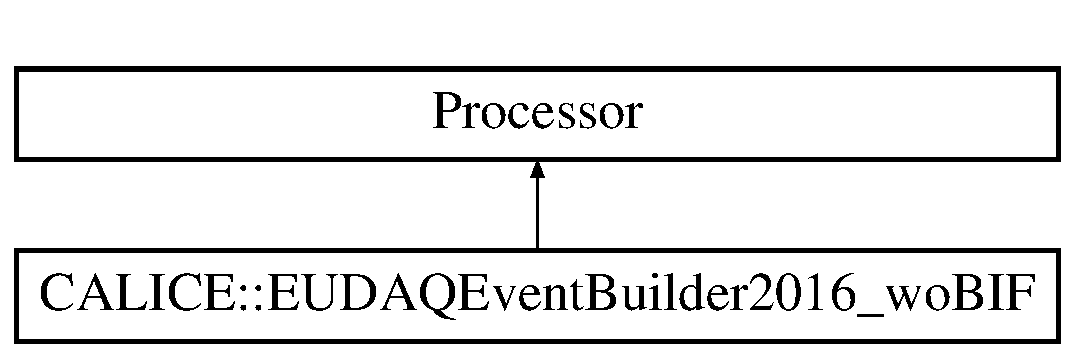
\includegraphics[height=2.000000cm]{classCALICE_1_1EUDAQEventBuilder2016__woBIF}
\end{center}
\end{figure}
\subsection*{Data Structures}
\begin{DoxyCompactItemize}
\item 
struct {\bf raw\-Data}
\begin{DoxyCompactList}\small\item\em The slcio data format. \end{DoxyCompactList}\item 
struct {\bf raw\-Data2016}
\begin{DoxyCompactList}\small\item\em The slcio data format. \end{DoxyCompactList}\item 
struct {\bf raw\-Temp}
\begin{DoxyCompactList}\small\item\em The slcio data format for the temperature sensor. \end{DoxyCompactList}\end{DoxyCompactItemize}
\subsection*{Public Member Functions}
\begin{DoxyCompactItemize}
\item 
virtual Processor $\ast$ {\bf new\-Processor} ()\label{classCALICE_1_1EUDAQEventBuilder2016__woBIF_a3a04c41b74e36f640aeb9c86ad3cdca8}

\begin{DoxyCompactList}\small\item\em Implementation of new Processor returns pointer to processor. \end{DoxyCompactList}\item 
void {\bf process\-Event} (L\-C\-Event $\ast$evt)\label{classCALICE_1_1EUDAQEventBuilder2016__woBIF_a60754bc616cb058327bbb2260cfe8528}

\begin{DoxyCompactList}\small\item\em Creates events with L\-C\-Genreal\-Object collections from the E\-U\-D\-A\-Q input file and calls all active processors' \doxyref{process\-Event()}{p.}{classCALICE_1_1EUDAQEventBuilder2016__woBIF_a60754bc616cb058327bbb2260cfe8528} and process\-Run\-Header Method. \end{DoxyCompactList}\item 
void {\bf write\-Slow\-Control} ()\label{classCALICE_1_1EUDAQEventBuilder2016__woBIF_a6e1ce5302228e32561144d460fd2c8b2}

\begin{DoxyCompactList}\small\item\em work on slow control data, A\-S\-I\-C \end{DoxyCompactList}\item 
virtual void {\bf init} ()
\begin{DoxyCompactList}\small\item\em work on slow control data, Temperature \end{DoxyCompactList}\item 
virtual void {\bf end} ()\label{classCALICE_1_1EUDAQEventBuilder2016__woBIF_ae20476a1150a4af6381ef71cb0876bb7}

\begin{DoxyCompactList}\small\item\em end method \end{DoxyCompactList}\item 
void {\bf print\-Parameters} ()\label{classCALICE_1_1EUDAQEventBuilder2016__woBIF_acca1cc6f9cb0f64884c5d57244678144}

\begin{DoxyCompactList}\small\item\em print parameters \end{DoxyCompactList}\end{DoxyCompactItemize}
\subsection*{Protected Attributes}
\begin{DoxyCompactItemize}
\item 
std\-::string {\bfseries \-\_\-input\-Col\-Name}\label{classCALICE_1_1EUDAQEventBuilder2016__woBIF_a148db24692f907ebffaa92d986f74abc}

\item 
std\-::string {\bfseries \-\_\-input\-Col\-Name\-Hodo1}\label{classCALICE_1_1EUDAQEventBuilder2016__woBIF_a32302f947a342f67aca9ad6a2602d336}

\item 
std\-::string {\bfseries \-\_\-input\-Col\-Name\-Hodo2}\label{classCALICE_1_1EUDAQEventBuilder2016__woBIF_a7cbfc6fc9c1f0f48ef4e197261242025}

\item 
std\-::string {\bfseries \-\_\-input\-Col\-Name\-Temp}\label{classCALICE_1_1EUDAQEventBuilder2016__woBIF_a034afc1da3f8a3454c608c6507f84bf1}

\item 
std\-::string {\bfseries \-\_\-output\-Col\-Name\-E\-C\-A\-L}\label{classCALICE_1_1EUDAQEventBuilder2016__woBIF_a2b0ea36b883a4a1869a55d33e72c8749}

\item 
std\-::string {\bfseries \-\_\-output\-Col\-Name\-H\-C\-A\-L}\label{classCALICE_1_1EUDAQEventBuilder2016__woBIF_a335d25ba8795d00757b12c74b8da6c9d}

\item 
std\-::string {\bfseries \-\_\-output\-Col\-Name\-Hodo1}\label{classCALICE_1_1EUDAQEventBuilder2016__woBIF_a0afcdeb1ec0cc83c5d004c8fa3e4e917}

\item 
std\-::string {\bfseries \-\_\-output\-Col\-Name\-Hodo2}\label{classCALICE_1_1EUDAQEventBuilder2016__woBIF_aab44581614ae469af9b7e41d567dc4e1}

\item 
std\-::string {\bfseries \-\_\-output\-Col\-Name\-Temp}\label{classCALICE_1_1EUDAQEventBuilder2016__woBIF_a2ac5a16ba93dfcf12fdd93f265eb69f0}

\item 
std\-::string {\bfseries \-\_\-detector\-Type\-Name}\label{classCALICE_1_1EUDAQEventBuilder2016__woBIF_a7c2d00b4dfbc4657e0f5054acfea275c}

\item 
int {\bf \-\_\-run\-Number}\label{classCALICE_1_1EUDAQEventBuilder2016__woBIF_a19285418aeb85d395bc2578ed33daea4}

\begin{DoxyCompactList}\small\item\em The run number. \end{DoxyCompactList}\end{DoxyCompactItemize}
\subsection*{Private Attributes}
\begin{DoxyCompactItemize}
\item 
int {\bfseries Lcio\-Event\-Nr}\label{classCALICE_1_1EUDAQEventBuilder2016__woBIF_a0902b1178ad8da54039cbc39947b3afb}

\item 
int {\bfseries discarded\-\_\-events}\label{classCALICE_1_1EUDAQEventBuilder2016__woBIF_a1664b7f6ac7161dafc2425a389b65606}

\item 
int {\bfseries all\-\_\-events}\label{classCALICE_1_1EUDAQEventBuilder2016__woBIF_ac93ee1a86efcfc6fc309dab046dbb82b}

\item 
bool {\bfseries temperaturecollection\-\_\-write}\label{classCALICE_1_1EUDAQEventBuilder2016__woBIF_a32d6b561a55fa2c4d1e25a94f9923bb0}

\end{DoxyCompactItemize}


\subsection{Detailed Description}
Processor for reading the A\-H\-C\-A\-L E\-U\-D\-A\-Q S\-L\-C\-I\-O files. 

It processes the input data to create events with L\-C\-I\-O collections of the A\-H\-C\-A\-L E\-U\-D\-A\-Q S\-L\-C\-I\-O output (sorted by readout cycles). Based on F. Gaede's Std\-Hep\-Reader to be found in the marlin package. \begin{DoxyAuthor}{Author}
\-: A. Irles (D\-E\-S\-Y), based on the S. Lu's (D\-E\-S\-Y Hamburg) Labview\-Converter2 
\end{DoxyAuthor}
\begin{DoxyDate}{Date}
May 20 2015 
\end{DoxyDate}


Definition at line 22 of file E\-U\-D\-A\-Q\-Event\-Builder2016\-\_\-wo\-B\-I\-F.\-hh.



\subsection{Member Function Documentation}
\index{C\-A\-L\-I\-C\-E\-::\-E\-U\-D\-A\-Q\-Event\-Builder2016\-\_\-wo\-B\-I\-F@{C\-A\-L\-I\-C\-E\-::\-E\-U\-D\-A\-Q\-Event\-Builder2016\-\_\-wo\-B\-I\-F}!init@{init}}
\index{init@{init}!CALICE::EUDAQEventBuilder2016_woBIF@{C\-A\-L\-I\-C\-E\-::\-E\-U\-D\-A\-Q\-Event\-Builder2016\-\_\-wo\-B\-I\-F}}
\subsubsection[{init}]{\setlength{\rightskip}{0pt plus 5cm}void C\-A\-L\-I\-C\-E\-::\-E\-U\-D\-A\-Q\-Event\-Builder2016\-\_\-wo\-B\-I\-F\-::init (
\begin{DoxyParamCaption}
{}
\end{DoxyParamCaption}
)\hspace{0.3cm}{\ttfamily [virtual]}}\label{classCALICE_1_1EUDAQEventBuilder2016__woBIF_a4a98304012c0359f80c26d9120ea807d}


work on slow control data, Temperature 

init method 

Definition at line 104 of file E\-U\-D\-A\-Q\-Event\-Builder2016\-\_\-wo\-B\-I\-F.\-cc.



References C\-A\-L\-I\-C\-E\-::\-E\-U\-D\-A\-Q\-Event\-Builder2016\-::print\-Parameters().



The documentation for this class was generated from the following files\-:\begin{DoxyCompactItemize}
\item 
E\-U\-D\-A\-Q\-Event\-Builder2016\-\_\-wo\-B\-I\-F.\-hh\item 
E\-U\-D\-A\-Q\-Event\-Builder2016\-\_\-wo\-B\-I\-F.\-cc\end{DoxyCompactItemize}

\section{C\-A\-L\-I\-C\-E\-:\-:E\-U\-D\-A\-Q\-Event\-Builder2018\-\_\-cosmics Class Reference}
\label{classCALICE_1_1EUDAQEventBuilder2018__cosmics}\index{C\-A\-L\-I\-C\-E\-::\-E\-U\-D\-A\-Q\-Event\-Builder2018\-\_\-cosmics@{C\-A\-L\-I\-C\-E\-::\-E\-U\-D\-A\-Q\-Event\-Builder2018\-\_\-cosmics}}


Processor for reading the A\-H\-C\-A\-L E\-U\-D\-A\-Q S\-L\-C\-I\-O files.  




{\ttfamily \#include $<$E\-U\-D\-A\-Q\-Event\-Builder2018\-\_\-cosmics.\-hh$>$}

Inheritance diagram for C\-A\-L\-I\-C\-E\-:\-:E\-U\-D\-A\-Q\-Event\-Builder2018\-\_\-cosmics\-:\begin{figure}[H]
\begin{center}
\leavevmode
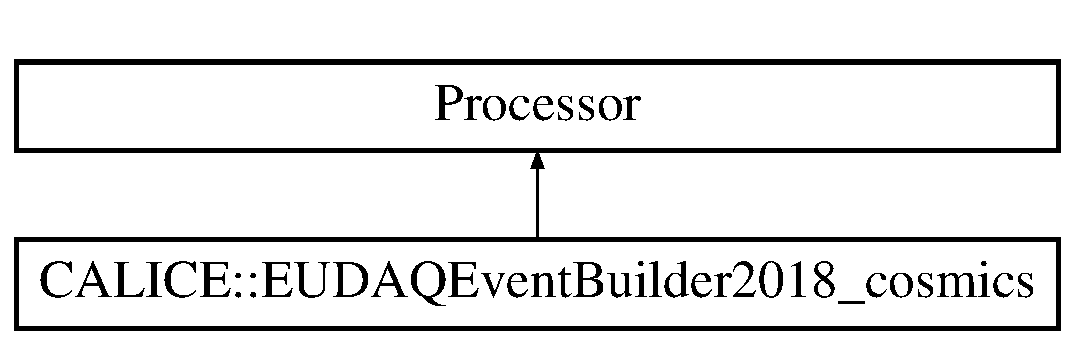
\includegraphics[height=2.000000cm]{classCALICE_1_1EUDAQEventBuilder2018__cosmics}
\end{center}
\end{figure}
\subsection*{Data Structures}
\begin{DoxyCompactItemize}
\item 
struct {\bf raw\-Data}
\begin{DoxyCompactList}\small\item\em The slcio data format. \end{DoxyCompactList}\item 
struct {\bf raw\-Data2016}
\begin{DoxyCompactList}\small\item\em The slcio data format. \end{DoxyCompactList}\item 
struct {\bf raw\-Temp}
\begin{DoxyCompactList}\small\item\em The slcio data format for the temperature sensor. \end{DoxyCompactList}\end{DoxyCompactItemize}
\subsection*{Public Member Functions}
\begin{DoxyCompactItemize}
\item 
virtual Processor $\ast$ {\bf new\-Processor} ()\label{classCALICE_1_1EUDAQEventBuilder2018__cosmics_a7357879bb180050f40062ca632441b25}

\begin{DoxyCompactList}\small\item\em Implementation of new Processor returns pointer to processor. \end{DoxyCompactList}\item 
void {\bf process\-Event} (L\-C\-Event $\ast$evt)\label{classCALICE_1_1EUDAQEventBuilder2018__cosmics_ad4a6f924ab44833e8e1a1ead3acb0265}

\begin{DoxyCompactList}\small\item\em Creates events with L\-C\-Genreal\-Object collections from the E\-U\-D\-A\-Q input file and calls all active processors' \doxyref{process\-Event()}{p.}{classCALICE_1_1EUDAQEventBuilder2018__cosmics_ad4a6f924ab44833e8e1a1ead3acb0265} and process\-Run\-Header Method. \end{DoxyCompactList}\item 
void {\bf write\-Slow\-Control} ()\label{classCALICE_1_1EUDAQEventBuilder2018__cosmics_a80621b89658e99fc4124dce8ed7ea18a}

\begin{DoxyCompactList}\small\item\em work on slow control data, A\-S\-I\-C \end{DoxyCompactList}\item 
virtual void {\bf init} ()
\begin{DoxyCompactList}\small\item\em work on slow control data, Temperature \end{DoxyCompactList}\item 
virtual void {\bf end} ()\label{classCALICE_1_1EUDAQEventBuilder2018__cosmics_a658729a9d275c4d79029f43cf12dc369}

\begin{DoxyCompactList}\small\item\em end method \end{DoxyCompactList}\item 
void {\bf print\-Parameters} ()\label{classCALICE_1_1EUDAQEventBuilder2018__cosmics_a2119bdb252323a67bcda8d42204bd03d}

\begin{DoxyCompactList}\small\item\em print parameters \end{DoxyCompactList}\end{DoxyCompactItemize}
\subsection*{Protected Attributes}
\begin{DoxyCompactItemize}
\item 
std\-::string {\bfseries \-\_\-input\-Col\-Name}\label{classCALICE_1_1EUDAQEventBuilder2018__cosmics_afa3f13aed5e59aecf2c965a88275b962}

\item 
std\-::string {\bfseries \-\_\-input\-Col\-Name\-Hodo1}\label{classCALICE_1_1EUDAQEventBuilder2018__cosmics_ae2c3b6766658ff7adb56fe24fa7a2a8a}

\item 
std\-::string {\bfseries \-\_\-input\-Col\-Name\-Hodo2}\label{classCALICE_1_1EUDAQEventBuilder2018__cosmics_a104213a036355f8238c65006b7f41f09}

\item 
std\-::string {\bfseries \-\_\-input\-Col\-Name\-Temp}\label{classCALICE_1_1EUDAQEventBuilder2018__cosmics_a80870e3d9842055bee7c7ea1cee4ce17}

\item 
std\-::string {\bfseries \-\_\-output\-Col\-Name\-E\-C\-A\-L}\label{classCALICE_1_1EUDAQEventBuilder2018__cosmics_aa7489e2126ff767326d24b99861bf615}

\item 
std\-::string {\bfseries \-\_\-output\-Col\-Name\-H\-C\-A\-L}\label{classCALICE_1_1EUDAQEventBuilder2018__cosmics_a4040953124cb9cd903fff698dc25d639}

\item 
std\-::string {\bfseries \-\_\-output\-Col\-Name\-Hodo1}\label{classCALICE_1_1EUDAQEventBuilder2018__cosmics_a06379f662fb5032d059c17f2d3e98987}

\item 
std\-::string {\bfseries \-\_\-output\-Col\-Name\-Hodo2}\label{classCALICE_1_1EUDAQEventBuilder2018__cosmics_a114a9d23b19871ca643e39a15100d2b0}

\item 
std\-::string {\bfseries \-\_\-output\-Col\-Name\-Temp}\label{classCALICE_1_1EUDAQEventBuilder2018__cosmics_a2990b7c5501541bcf4450f492b262351}

\item 
std\-::string {\bfseries \-\_\-detector\-Type\-Name}\label{classCALICE_1_1EUDAQEventBuilder2018__cosmics_a66b1bf45f6c32f1efba2af6af7aca4a8}

\item 
int {\bf \-\_\-run\-Number}\label{classCALICE_1_1EUDAQEventBuilder2018__cosmics_ad987ff19dc97413e687cc97dd7c559d3}

\begin{DoxyCompactList}\small\item\em The run number. \end{DoxyCompactList}\end{DoxyCompactItemize}
\subsection*{Private Attributes}
\begin{DoxyCompactItemize}
\item 
int {\bfseries Lcio\-Event\-Nr}\label{classCALICE_1_1EUDAQEventBuilder2018__cosmics_a492c27b52ae835beee0690feb93ddf77}

\item 
int {\bfseries discarded\-\_\-events}\label{classCALICE_1_1EUDAQEventBuilder2018__cosmics_a40ab39464bbef828d05217325b281aa3}

\item 
int {\bfseries all\-\_\-events}\label{classCALICE_1_1EUDAQEventBuilder2018__cosmics_afc5c87eec1814fdfa07f3babde043bad}

\item 
bool {\bfseries temperaturecollection\-\_\-write}\label{classCALICE_1_1EUDAQEventBuilder2018__cosmics_a0f1c95b600decec735998ce6451855e6}

\end{DoxyCompactItemize}


\subsection{Detailed Description}
Processor for reading the A\-H\-C\-A\-L E\-U\-D\-A\-Q S\-L\-C\-I\-O files. 

It processes the input data to create events with L\-C\-I\-O collections of the A\-H\-C\-A\-L E\-U\-D\-A\-Q S\-L\-C\-I\-O output (sorted by readout cycles). Based on F. Gaede's Std\-Hep\-Reader to be found in the marlin package. \begin{DoxyAuthor}{Author}
\-: A. Irles (D\-E\-S\-Y), based on the S. Lu's (D\-E\-S\-Y Hamburg) Labview\-Converter2 
\end{DoxyAuthor}
\begin{DoxyDate}{Date}
May 20 2015 
\end{DoxyDate}


Definition at line 22 of file E\-U\-D\-A\-Q\-Event\-Builder2018\-\_\-cosmics.\-hh.



\subsection{Member Function Documentation}
\index{C\-A\-L\-I\-C\-E\-::\-E\-U\-D\-A\-Q\-Event\-Builder2018\-\_\-cosmics@{C\-A\-L\-I\-C\-E\-::\-E\-U\-D\-A\-Q\-Event\-Builder2018\-\_\-cosmics}!init@{init}}
\index{init@{init}!CALICE::EUDAQEventBuilder2018_cosmics@{C\-A\-L\-I\-C\-E\-::\-E\-U\-D\-A\-Q\-Event\-Builder2018\-\_\-cosmics}}
\subsubsection[{init}]{\setlength{\rightskip}{0pt plus 5cm}void C\-A\-L\-I\-C\-E\-::\-E\-U\-D\-A\-Q\-Event\-Builder2018\-\_\-cosmics\-::init (
\begin{DoxyParamCaption}
{}
\end{DoxyParamCaption}
)\hspace{0.3cm}{\ttfamily [virtual]}}\label{classCALICE_1_1EUDAQEventBuilder2018__cosmics_acc4e1a445d624669c60bed1bbb995969}


work on slow control data, Temperature 

init method 

Definition at line 107 of file E\-U\-D\-A\-Q\-Event\-Builder2018\-\_\-cosmics.\-cc.



References C\-A\-L\-I\-C\-E\-::\-E\-U\-D\-A\-Q\-Event\-Builder2016\-\_\-wo\-B\-I\-F\-::print\-Parameters().



The documentation for this class was generated from the following files\-:\begin{DoxyCompactItemize}
\item 
E\-U\-D\-A\-Q\-Event\-Builder2018\-\_\-cosmics.\-hh\item 
E\-U\-D\-A\-Q\-Event\-Builder2018\-\_\-cosmics.\-cc\end{DoxyCompactItemize}

\section{C\-A\-L\-I\-C\-E\-:\-:E\-U\-D\-A\-Q\-Temp\-Sensor\-Block Class Reference}
\label{classCALICE_1_1EUDAQTempSensorBlock}\index{C\-A\-L\-I\-C\-E\-::\-E\-U\-D\-A\-Q\-Temp\-Sensor\-Block@{C\-A\-L\-I\-C\-E\-::\-E\-U\-D\-A\-Q\-Temp\-Sensor\-Block}}


Class for the temperature sensor data as acquired by the A\-H\-C\-A\-L E\-U\-D\-A\-Q.  




{\ttfamily \#include $<$E\-U\-D\-A\-Q\-Temp\-Sensor\-Block.\-hh$>$}

Inheritance diagram for C\-A\-L\-I\-C\-E\-:\-:E\-U\-D\-A\-Q\-Temp\-Sensor\-Block\-:\begin{figure}[H]
\begin{center}
\leavevmode
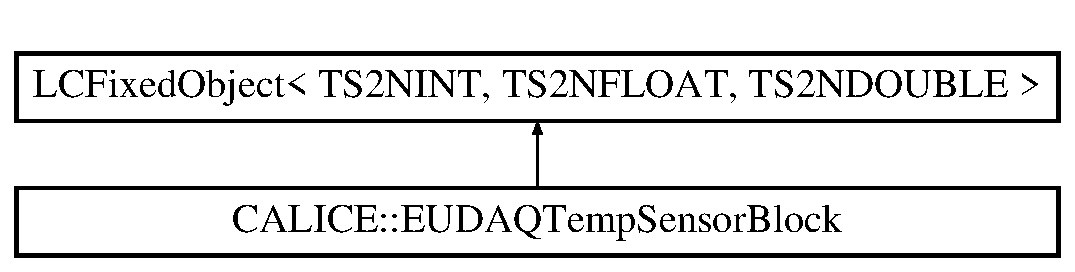
\includegraphics[height=2.000000cm]{classCALICE_1_1EUDAQTempSensorBlock}
\end{center}
\end{figure}
\subsection*{Public Member Functions}
\begin{DoxyCompactItemize}
\item 
{\bf E\-U\-D\-A\-Q\-Temp\-Sensor\-Block} (int L\-D\-A\-Number, int Port\-Number, int T1, int T2, int T3, int T4, int T5, int T6, int T\-D\-I\-F, int T\-P\-W\-R)\label{classCALICE_1_1EUDAQTempSensorBlock_ae02d2597a925e3e7fd290a0b31d685c3}

\begin{DoxyCompactList}\small\item\em Convenient c'tor. \end{DoxyCompactList}\item 
{\bf E\-U\-D\-A\-Q\-Temp\-Sensor\-Block} (L\-C\-Object $\ast$obj)\label{classCALICE_1_1EUDAQTempSensorBlock_ac20c9533a2640ee57f741cfca85937eb}

\begin{DoxyCompactList}\small\item\em 'Copy constructor' needed to interpret L\-C\-Collection read from file/database. \end{DoxyCompactList}\item 
virtual {\bf $\sim$\-E\-U\-D\-A\-Q\-Temp\-Sensor\-Block} ()\label{classCALICE_1_1EUDAQTempSensorBlock_a482b674c4674680f57ad441d32d3e7f6}

\begin{DoxyCompactList}\small\item\em Important for memory handling. \end{DoxyCompactList}\item 
int {\bfseries Get\-L\-D\-A\-Number} () const \label{classCALICE_1_1EUDAQTempSensorBlock_ae2f5861ac123e152117d8086d260ed28}

\item 
int {\bfseries Get\-Port\-Number} () const \label{classCALICE_1_1EUDAQTempSensorBlock_aa85c8473e68609696ef73732ce2e1c73}

\item 
int {\bfseries Get\-T1} () const \label{classCALICE_1_1EUDAQTempSensorBlock_a05f7d3cd2f61b94b7b355dad9ed04e71}

\item 
int {\bfseries Get\-T2} () const \label{classCALICE_1_1EUDAQTempSensorBlock_a57fceddca009de039005ae35728279bf}

\item 
int {\bfseries Get\-T3} () const \label{classCALICE_1_1EUDAQTempSensorBlock_abfa60426a963bcd31243be0e472451bd}

\item 
int {\bfseries Get\-T4} () const \label{classCALICE_1_1EUDAQTempSensorBlock_a02a094c6b095e4aa1a813ba6027b039b}

\item 
int {\bfseries Get\-T5} () const \label{classCALICE_1_1EUDAQTempSensorBlock_a7dcee9102c3faddf788cb26584bd991f}

\item 
int {\bfseries Get\-T6} () const \label{classCALICE_1_1EUDAQTempSensorBlock_a8dc023707cd85d0617ac89f9ccd04f91}

\item 
int {\bfseries Get\-T\-D\-I\-F} () const \label{classCALICE_1_1EUDAQTempSensorBlock_a84eecef47e27057ca1a52c2a771f65ec}

\item 
int {\bfseries Get\-T\-P\-W\-R} () const \label{classCALICE_1_1EUDAQTempSensorBlock_a5f8f3e5ed6e1dafbd2bd2e5a6c571ded}

\item 
void {\bfseries print} (std\-::ostream \&os, int)\label{classCALICE_1_1EUDAQTempSensorBlock_a573889f528e77c39321d3042d8715301}

\item 
const std\-::string {\bf get\-Type\-Name} () const \label{classCALICE_1_1EUDAQTempSensorBlock_aaf80776bd59b87c45ef15e10316142c4}

\begin{DoxyCompactList}\small\item\em Return the type of the class. \end{DoxyCompactList}\item 
const std\-::string {\bf get\-Data\-Description} () const \label{classCALICE_1_1EUDAQTempSensorBlock_a63392b2373970e5d7d4854f5027a96ec}

\begin{DoxyCompactList}\small\item\em Return a brief description of the data members. \end{DoxyCompactList}\end{DoxyCompactItemize}


\subsection{Detailed Description}
Class for the temperature sensor data as acquired by the A\-H\-C\-A\-L E\-U\-D\-A\-Q. 

The class reflects that the data are received in the E\-U\-D\-A\-Q \begin{DoxyAuthor}{Author}
A. Irles D\-E\-S\-Y Hamburg, based on \doxyref{Temp\-Sensor\-Block}{p.}{classCALICE_1_1TempSensorBlock} by S. Lu (date Dec 17 2012) 
\end{DoxyAuthor}
\begin{DoxyDate}{Date}
25june 2015 
\end{DoxyDate}


Definition at line 23 of file E\-U\-D\-A\-Q\-Temp\-Sensor\-Block.\-hh.



The documentation for this class was generated from the following file\-:\begin{DoxyCompactItemize}
\item 
E\-U\-D\-A\-Q\-Temp\-Sensor\-Block.\-hh\end{DoxyCompactItemize}

\section{C\-A\-L\-I\-C\-E\-:\-:Event\-Checker Class Reference}
\label{classCALICE_1_1EventChecker}\index{C\-A\-L\-I\-C\-E\-::\-Event\-Checker@{C\-A\-L\-I\-C\-E\-::\-Event\-Checker}}


Class to process Labview raw.  




{\ttfamily \#include $<$Event\-Checker.\-hh$>$}

Inheritance diagram for C\-A\-L\-I\-C\-E\-:\-:Event\-Checker\-:\begin{figure}[H]
\begin{center}
\leavevmode
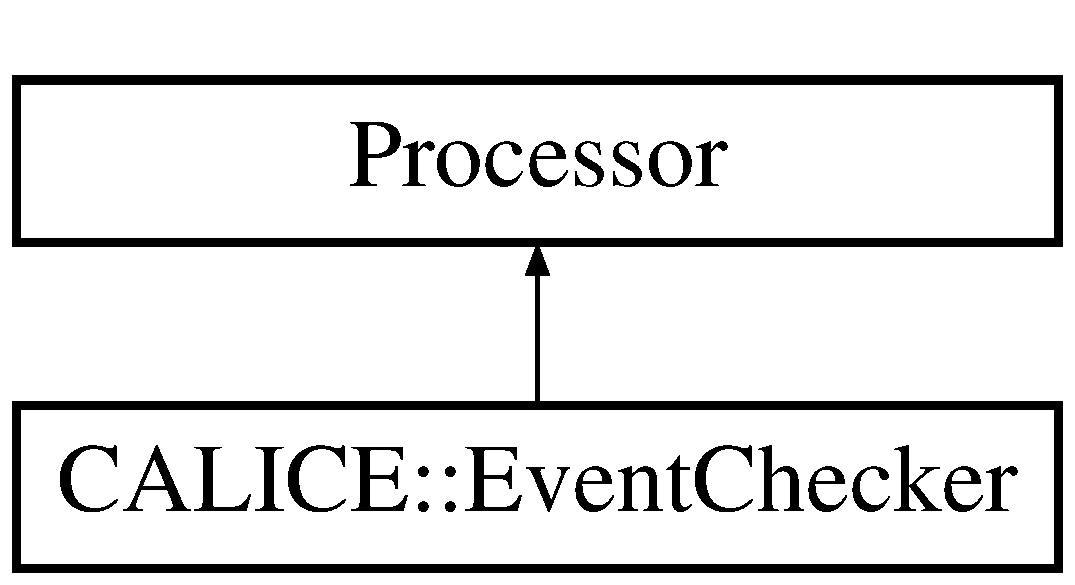
\includegraphics[height=2.000000cm]{classCALICE_1_1EventChecker}
\end{center}
\end{figure}
\subsection*{Public Member Functions}
\begin{DoxyCompactItemize}
\item 
virtual Processor $\ast$ {\bfseries new\-Processor} ()\label{classCALICE_1_1EventChecker_af20da755dd41779a95fc39934a69610d}

\item 
void {\bfseries init} ()\label{classCALICE_1_1EventChecker_ab41fa998c1d7ba6fe042e431578cb8e9}

\item 
void {\bfseries process\-Event} (L\-C\-Event $\ast$evt)\label{classCALICE_1_1EventChecker_a6419a5663a9eb46524bd9b8401d812e4}

\item 
void {\bfseries end} ()\label{classCALICE_1_1EventChecker_a34dd62a9bdd384b2a5bb9fc59b3634d5}

\end{DoxyCompactItemize}
\subsection*{Protected Attributes}
\begin{DoxyCompactItemize}
\item 
std\-::string {\bfseries \-\_\-input\-Col\-Name}\label{classCALICE_1_1EventChecker_a94fd86833f389b2eaf23cce14baef4bb}

\end{DoxyCompactItemize}


\subsection{Detailed Description}
Class to process Labview raw. 

\begin{DoxyAuthor}{Author}
\-: Shaojun Lu D\-E\-S\-Y 
\end{DoxyAuthor}
\begin{DoxyDate}{Date}
Nov 15 2012 
\end{DoxyDate}


Definition at line 19 of file Event\-Checker.\-hh.



The documentation for this class was generated from the following files\-:\begin{DoxyCompactItemize}
\item 
Event\-Checker.\-hh\item 
Event\-Checker.\-cc\end{DoxyCompactItemize}

\section{C\-A\-L\-I\-C\-E\-:\-:H\-B\-U\-Temperature\-Block Class Reference}
\label{classCALICE_1_1HBUTemperatureBlock}\index{C\-A\-L\-I\-C\-E\-::\-H\-B\-U\-Temperature\-Block@{C\-A\-L\-I\-C\-E\-::\-H\-B\-U\-Temperature\-Block}}


Class for the Labview Data as acquired by the A\-H\-C\-A\-L Labview.  




{\ttfamily \#include $<$H\-B\-Utemperature\-Block.\-hh$>$}

Inheritance diagram for C\-A\-L\-I\-C\-E\-:\-:H\-B\-U\-Temperature\-Block\-:\begin{figure}[H]
\begin{center}
\leavevmode
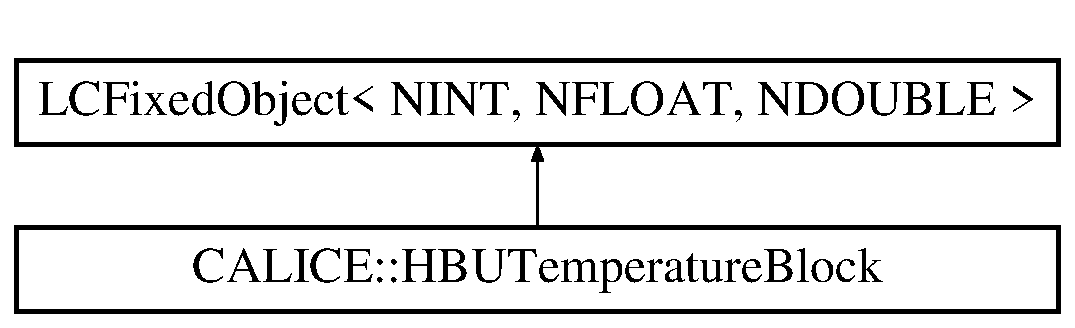
\includegraphics[height=2.000000cm]{classCALICE_1_1HBUTemperatureBlock}
\end{center}
\end{figure}
\subsection*{Public Member Functions}
\begin{DoxyCompactItemize}
\item 
{\bf H\-B\-U\-Temperature\-Block} (float temp1, float temp2, float temp3, float temp4, float temp5, float temp6)\label{classCALICE_1_1HBUTemperatureBlock_a31c53d802bbe9d3d4ab67b89bcea84d9}

\begin{DoxyCompactList}\small\item\em Convenient c'tor. \end{DoxyCompactList}\item 
{\bf H\-B\-U\-Temperature\-Block} (L\-C\-Object $\ast$obj)\label{classCALICE_1_1HBUTemperatureBlock_a66aa0df1cd4816dc5a05993af1fcb20f}

\begin{DoxyCompactList}\small\item\em 'Copy constructor' needed to interpret L\-C\-Collection read from file/database. \end{DoxyCompactList}\item 
virtual {\bf $\sim$\-H\-B\-U\-Temperature\-Block} ()\label{classCALICE_1_1HBUTemperatureBlock_a990d55a7677c5410beb42efb680d5a6d}

\begin{DoxyCompactList}\small\item\em Important for memory handling. \end{DoxyCompactList}\item 
int {\bf Get\-Temperature} (int i) const \label{classCALICE_1_1HBUTemperatureBlock_a651fe2deafbd2658dafa95457a2883c9}

\begin{DoxyCompactList}\small\item\em get the i\-Th temperature value. \end{DoxyCompactList}\item 
void {\bf print} (std\-::ostream \&os, int)\label{classCALICE_1_1HBUTemperatureBlock_a9c8cbfa1f0cce53c37f4713301ac9106}

\begin{DoxyCompactList}\small\item\em Convenient print method. \end{DoxyCompactList}\item 
const std\-::string {\bf get\-Type\-Name} () const \label{classCALICE_1_1HBUTemperatureBlock_ab15e48bcf14a740d241ec60e3ee03677}

\begin{DoxyCompactList}\small\item\em Return the type of the class. \end{DoxyCompactList}\item 
const std\-::string {\bf get\-Data\-Description} () const \label{classCALICE_1_1HBUTemperatureBlock_ae010246fa7084166bee5a5bcb83957c0}

\begin{DoxyCompactList}\small\item\em Return a brief description of the data members. \end{DoxyCompactList}\end{DoxyCompactItemize}


\subsection{Detailed Description}
Class for the Labview Data as acquired by the A\-H\-C\-A\-L Labview. 

The class reflects that the data are received in the Labview \begin{DoxyAuthor}{Author}
S. Lu D\-E\-S\-Y Hamburg 
\end{DoxyAuthor}
\begin{DoxyDate}{Date}
Oct 02 2012 
\end{DoxyDate}


Definition at line 23 of file H\-B\-Utemperature\-Block.\-hh.



The documentation for this class was generated from the following file\-:\begin{DoxyCompactItemize}
\item 
H\-B\-Utemperature\-Block.\-hh\end{DoxyCompactItemize}

\section{C\-A\-L\-I\-C\-E\-:\-:Labview\-Block Class Reference}
\label{classCALICE_1_1LabviewBlock}\index{C\-A\-L\-I\-C\-E\-::\-Labview\-Block@{C\-A\-L\-I\-C\-E\-::\-Labview\-Block}}


Class for the Labview Data as acquired by the A\-H\-C\-A\-L Labview.  




{\ttfamily \#include $<$Labview\-Block.\-hh$>$}

Inheritance diagram for C\-A\-L\-I\-C\-E\-:\-:Labview\-Block\-:\begin{figure}[H]
\begin{center}
\leavevmode
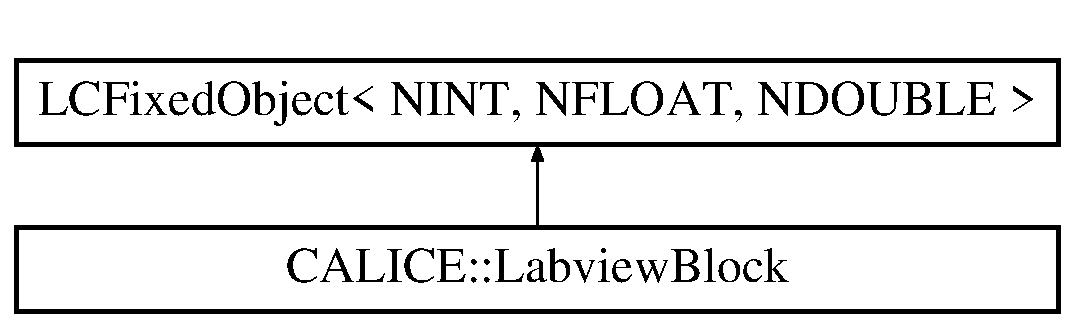
\includegraphics[height=2.000000cm]{classCALICE_1_1LabviewBlock}
\end{center}
\end{figure}
\subsection*{Public Member Functions}
\begin{DoxyCompactItemize}
\item 
{\bf Labview\-Block} (int Bunch\-X\-I\-D, int Cycle\-Nr, int Chip\-I\-D, int A\-S\-I\-C\-Nr, int Evt\-Nr, int Channel, int T\-D\-C, int A\-D\-C, int X\-Pos, int Y\-Pos, int Hit\-Bit, int Gain\-Bit)\label{classCALICE_1_1LabviewBlock_acadd794d318b2fc9132a20547107c499}

\begin{DoxyCompactList}\small\item\em Convenient c'tor. \end{DoxyCompactList}\item 
{\bf Labview\-Block} (L\-C\-Object $\ast$obj)\label{classCALICE_1_1LabviewBlock_ae8ff897ba24df56660d05a043768cb15}

\begin{DoxyCompactList}\small\item\em 'Copy constructor' needed to interpret L\-C\-Collection read from file/database. \end{DoxyCompactList}\item 
virtual {\bf $\sim$\-Labview\-Block} ()\label{classCALICE_1_1LabviewBlock_af2c2454dec16e14d52fd44545e06f3a9}

\begin{DoxyCompactList}\small\item\em Important for memory handling. \end{DoxyCompactList}\item 
int {\bf Get\-Bunch\-X\-I\-D} () const \label{classCALICE_1_1LabviewBlock_a94583fba9cc6196c89728b850e5f13b5}

\begin{DoxyCompactList}\small\item\em get the Bunch\-X\-I\-D. \end{DoxyCompactList}\item 
int {\bf Get\-Cycle\-Nr} () const \label{classCALICE_1_1LabviewBlock_ae8c915a57a7144c79521a2bd2562e8de}

\begin{DoxyCompactList}\small\item\em get the Cycle\-Nr. \end{DoxyCompactList}\item 
int {\bf Get\-Chip\-I\-D} () const \label{classCALICE_1_1LabviewBlock_a5c14f61678c97e36a4c63717055175b3}

\begin{DoxyCompactList}\small\item\em get the Chip\-I\-D. \end{DoxyCompactList}\item 
int {\bf Get\-A\-S\-I\-C\-Nr} () const \label{classCALICE_1_1LabviewBlock_a20b34eb84745f2fb035daebcec6c8eb8}

\begin{DoxyCompactList}\small\item\em get the A\-S\-I\-C\-Nr. \end{DoxyCompactList}\item 
int {\bf Get\-Evt\-Nr} () const \label{classCALICE_1_1LabviewBlock_a15229cd3b6b44ef7fcabb3d7f8b7cbf4}

\begin{DoxyCompactList}\small\item\em get the Evt\-Nr. \end{DoxyCompactList}\item 
int {\bf Get\-Channel} () const \label{classCALICE_1_1LabviewBlock_a56f8ebcbbff0a314b7b647900e677549}

\begin{DoxyCompactList}\small\item\em get the Channel. \end{DoxyCompactList}\item 
int {\bf Get\-T\-D\-C} () const \label{classCALICE_1_1LabviewBlock_aabb31d4cb06168df0acd5126b05ad801}

\begin{DoxyCompactList}\small\item\em get the T\-D\-C. \end{DoxyCompactList}\item 
int {\bf Get\-A\-D\-C} () const \label{classCALICE_1_1LabviewBlock_a1f4937a4b2e883ecf0364b7369cd3708}

\begin{DoxyCompactList}\small\item\em get the A\-D\-C. \end{DoxyCompactList}\item 
int {\bf Get\-X\-Pos} () const \label{classCALICE_1_1LabviewBlock_aeb75ea8ea414ef184e30d8c6a967a5f6}

\begin{DoxyCompactList}\small\item\em get the X\-Pos. \end{DoxyCompactList}\item 
int {\bf Get\-Y\-Pos} () const \label{classCALICE_1_1LabviewBlock_a42495a34bc8c54fd5f26a8de2eb17584}

\begin{DoxyCompactList}\small\item\em get the Y\-Pos. \end{DoxyCompactList}\item 
int {\bf Get\-Hit\-Bit} () const \label{classCALICE_1_1LabviewBlock_abcf1f2fcce69be90c406ac96d2a960df}

\begin{DoxyCompactList}\small\item\em get the Hit\-Bit. \end{DoxyCompactList}\item 
int {\bf Get\-Gain\-Bit} () const \label{classCALICE_1_1LabviewBlock_adc2f3d040d21a1988569a6e4dd383f2e}

\begin{DoxyCompactList}\small\item\em get the Gain\-Bit. \end{DoxyCompactList}\item 
void {\bf print} (std\-::ostream \&os, int)\label{classCALICE_1_1LabviewBlock_ad1ac4cf349c76f815a0e0514aec496d6}

\begin{DoxyCompactList}\small\item\em Convenient print method. \end{DoxyCompactList}\item 
const std\-::string {\bf get\-Type\-Name} () const \label{classCALICE_1_1LabviewBlock_ad5cfc916c66f1211bcf189237473eba6}

\begin{DoxyCompactList}\small\item\em Return the type of the class. \end{DoxyCompactList}\item 
const std\-::string {\bf get\-Data\-Description} () const \label{classCALICE_1_1LabviewBlock_a569668ec05207ba78574d45acce7e93a}

\begin{DoxyCompactList}\small\item\em Return a brief description of the data members. \end{DoxyCompactList}\end{DoxyCompactItemize}


\subsection{Detailed Description}
Class for the Labview Data as acquired by the A\-H\-C\-A\-L Labview. 

The class reflects that the data are received in the Labview \begin{DoxyAuthor}{Author}
S. Lu D\-E\-S\-Y Hamburg 
\end{DoxyAuthor}
\begin{DoxyDate}{Date}
Aug 16 2012 
\end{DoxyDate}


Definition at line 23 of file Labview\-Block.\-hh.



The documentation for this class was generated from the following file\-:\begin{DoxyCompactItemize}
\item 
Labview\-Block.\-hh\end{DoxyCompactItemize}

\section{C\-A\-L\-I\-C\-E\-:\-:Labview\-Block2 Class Reference}
\label{classCALICE_1_1LabviewBlock2}\index{C\-A\-L\-I\-C\-E\-::\-Labview\-Block2@{C\-A\-L\-I\-C\-E\-::\-Labview\-Block2}}


Class for the Labview Data as acquired by the A\-H\-C\-A\-L Labview.  




{\ttfamily \#include $<$Labview\-Block2.\-hh$>$}

Inheritance diagram for C\-A\-L\-I\-C\-E\-:\-:Labview\-Block2\-:\begin{figure}[H]
\begin{center}
\leavevmode
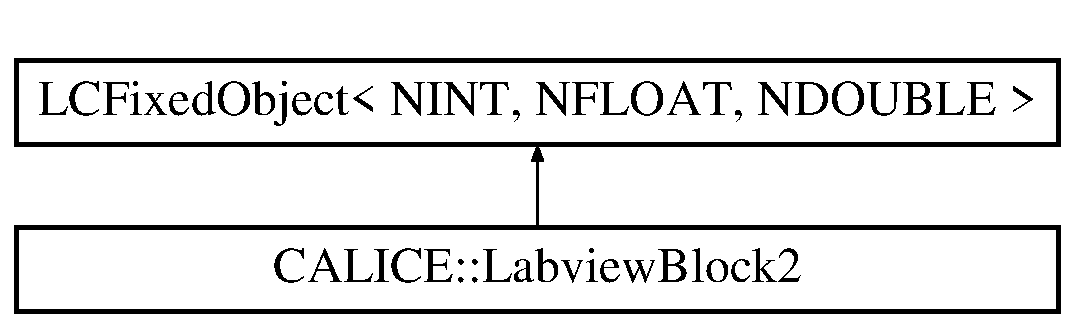
\includegraphics[height=2.000000cm]{classCALICE_1_1LabviewBlock2}
\end{center}
\end{figure}
\subsection*{Public Member Functions}
\begin{DoxyCompactItemize}
\item 
{\bf Labview\-Block2} (int Cycle\-Nr, int Bunch\-X\-I\-D, int Chip\-I\-D, int Evt\-Nr, int Channel, int T\-D\-C, int A\-D\-C, int Hit\-Bit, int Gain\-Bit)\label{classCALICE_1_1LabviewBlock2_aa409f51a0803d4ca5e6fe15204262118}

\begin{DoxyCompactList}\small\item\em Convenient c'tor. \end{DoxyCompactList}\item 
{\bf Labview\-Block2} (L\-C\-Object $\ast$obj)\label{classCALICE_1_1LabviewBlock2_acb5c7d7d0a0d9aecff3434f8b712745d}

\begin{DoxyCompactList}\small\item\em 'Copy constructor' needed to interpret L\-C\-Collection read from file/database. \end{DoxyCompactList}\item 
virtual {\bf $\sim$\-Labview\-Block2} ()\label{classCALICE_1_1LabviewBlock2_aabc7bc093f568a532a4cf7097a84fb99}

\begin{DoxyCompactList}\small\item\em Important for memory handling. \end{DoxyCompactList}\item 
int {\bf Get\-Cycle\-Nr} () const \label{classCALICE_1_1LabviewBlock2_aabd11e4b300c4a3644ff5fbbf513af36}

\begin{DoxyCompactList}\small\item\em get the Cycle\-Nr. \end{DoxyCompactList}\item 
int {\bf Get\-Bunch\-X\-I\-D} () const \label{classCALICE_1_1LabviewBlock2_ae25025f2f9bc95883c2d6b23d38ecc8e}

\begin{DoxyCompactList}\small\item\em get the Bunch\-X\-I\-D. \end{DoxyCompactList}\item 
int {\bf Get\-Chip\-I\-D} () const \label{classCALICE_1_1LabviewBlock2_a6e1e7613bbf370e6a0e11ef3896bb6f9}

\begin{DoxyCompactList}\small\item\em get the Chip\-I\-D. \end{DoxyCompactList}\item 
int {\bf Get\-Evt\-Nr} () const \label{classCALICE_1_1LabviewBlock2_a8d4a67989cad5bf504971abc612653cc}

\begin{DoxyCompactList}\small\item\em get the Evt\-Nr. \end{DoxyCompactList}\item 
int {\bf Get\-Channel} () const \label{classCALICE_1_1LabviewBlock2_a9636e5feb9a0cba799067f7b2390d25b}

\begin{DoxyCompactList}\small\item\em get the Channel. \end{DoxyCompactList}\item 
int {\bf Get\-T\-D\-C} () const \label{classCALICE_1_1LabviewBlock2_a57d069ac572fbc56de3abfaaa007eb6e}

\begin{DoxyCompactList}\small\item\em get the T\-D\-C. \end{DoxyCompactList}\item 
int {\bf Get\-A\-D\-C} () const \label{classCALICE_1_1LabviewBlock2_ab3d5c72af2f3fa8dd180afb091455dee}

\begin{DoxyCompactList}\small\item\em get the A\-D\-C. \end{DoxyCompactList}\item 
int {\bf Get\-Hit\-Bit} () const \label{classCALICE_1_1LabviewBlock2_a98de016fe2fa0639ca0cc82b1eecf97f}

\begin{DoxyCompactList}\small\item\em get the Hit\-Bit. \end{DoxyCompactList}\item 
int {\bf Get\-Gain\-Bit} () const \label{classCALICE_1_1LabviewBlock2_a08c27201d04e385c9be5709ce2fb9525}

\begin{DoxyCompactList}\small\item\em get the Gain\-Bit. \end{DoxyCompactList}\item 
void {\bf print} (std\-::ostream \&os, int)\label{classCALICE_1_1LabviewBlock2_a7cb31b570b9ba0054b44af4ef8402158}

\begin{DoxyCompactList}\small\item\em Convenient print method. \end{DoxyCompactList}\item 
const std\-::string {\bf get\-Type\-Name} () const \label{classCALICE_1_1LabviewBlock2_a76502d161af6719c26997c8636fc5fa3}

\begin{DoxyCompactList}\small\item\em Return the type of the class. \end{DoxyCompactList}\item 
const std\-::string {\bf get\-Data\-Description} () const \label{classCALICE_1_1LabviewBlock2_aca62c674b9814b65e27baa3b8d11b5dc}

\begin{DoxyCompactList}\small\item\em Return a brief description of the data members. \end{DoxyCompactList}\end{DoxyCompactItemize}


\subsection{Detailed Description}
Class for the Labview Data as acquired by the A\-H\-C\-A\-L Labview. 

The class reflects that the data are received in the Labview \begin{DoxyAuthor}{Author}
S. Lu D\-E\-S\-Y Hamburg 
\end{DoxyAuthor}
\begin{DoxyDate}{Date}
Mar 20 2014 Created for New Labview data format. 
\end{DoxyDate}


Definition at line 24 of file Labview\-Block2.\-hh.



The documentation for this class was generated from the following file\-:\begin{DoxyCompactItemize}
\item 
Labview\-Block2.\-hh\end{DoxyCompactItemize}

\section{marlin\-:\-:Labview\-Converter Class Reference}
\label{classmarlin_1_1LabviewConverter}\index{marlin\-::\-Labview\-Converter@{marlin\-::\-Labview\-Converter}}


Processor for reading the A\-H\-C\-A\-L Labview asscii files.  




{\ttfamily \#include $<$Labview\-Converter.\-hh$>$}

Inheritance diagram for marlin\-:\-:Labview\-Converter\-:\begin{figure}[H]
\begin{center}
\leavevmode
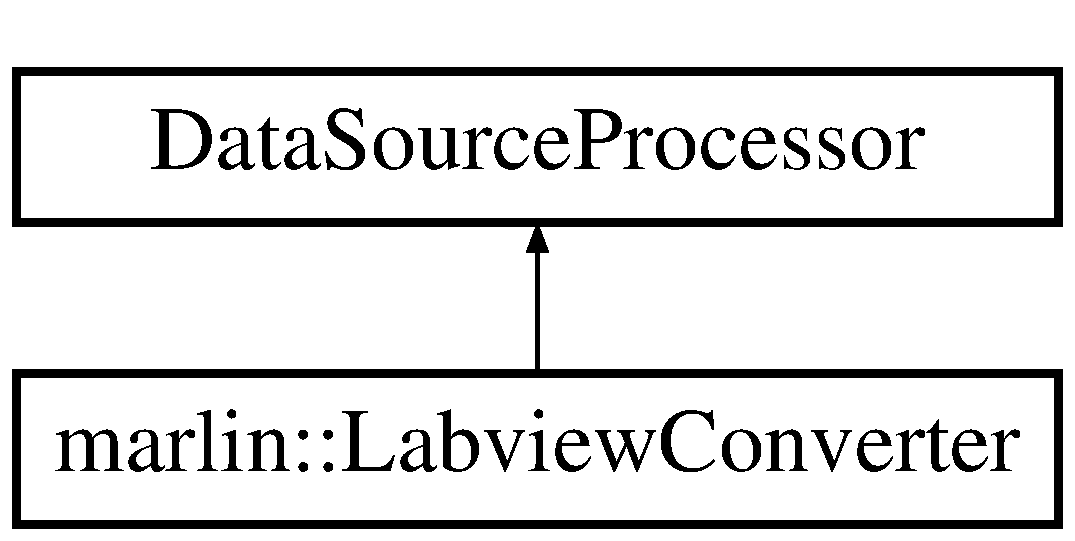
\includegraphics[height=2.000000cm]{classmarlin_1_1LabviewConverter}
\end{center}
\end{figure}
\subsection*{Public Member Functions}
\begin{DoxyCompactItemize}
\item 
virtual {\bf Labview\-Converter} $\ast$ {\bf new\-Processor} ()\label{classmarlin_1_1LabviewConverter_ac445a8f712cbc96fd9f90c190dad8347}

\begin{DoxyCompactList}\small\item\em Implementation of new Processor returns pointer to processor. \end{DoxyCompactList}\item 
virtual void {\bf read\-Data\-Source} (int num\-Events)\label{classmarlin_1_1LabviewConverter_ad865613e9671e541a1e64ecd8c9c897b}

\begin{DoxyCompactList}\small\item\em Creates events with L\-C\-Genreal\-Object collections from the Labview input file and calls all active processors' process\-Event() and process\-Run\-Header Method. \end{DoxyCompactList}\item 
void {\bf write\-Slow\-Control} ()\label{classmarlin_1_1LabviewConverter_a3e5cfb39a19c0ca17ac3ecdb3c9f85e7}

\begin{DoxyCompactList}\small\item\em work on slow control data, A\-S\-I\-C \end{DoxyCompactList}\item 
virtual void {\bf init} ()
\begin{DoxyCompactList}\small\item\em work on slow control data, Temperature \end{DoxyCompactList}\item 
virtual void {\bf end} ()\label{classmarlin_1_1LabviewConverter_ae1700a9004281db26476d22b5cc7c10b}

\begin{DoxyCompactList}\small\item\em end method \end{DoxyCompactList}\end{DoxyCompactItemize}
\subsection*{Protected Attributes}
\begin{DoxyCompactItemize}
\item 
std\-::string {\bf \-\_\-ofile}
\begin{DoxyCompactList}\small\item\em The string variable to access the data. \end{DoxyCompactList}\item 
std\-::string {\bf \-\_\-data}\label{classmarlin_1_1LabviewConverter_a2a7a7963f225275d1b19989c356f4f9a}

\begin{DoxyCompactList}\small\item\em The string variable to access the data. \end{DoxyCompactList}\item 
int {\bf \-\_\-run\-Number}\label{classmarlin_1_1LabviewConverter_aeefca366348efb5bf87b819ec8807132}

\begin{DoxyCompactList}\small\item\em The run number. \end{DoxyCompactList}\item 
int {\bf \-\_\-\-Slow\-Control\-Line\-Number}\label{classmarlin_1_1LabviewConverter_ab280114ab31d4ff2bedfea28ec3a7fc8}

\begin{DoxyCompactList}\small\item\em Slow control line number, H\-B\-U\-: 120, E\-P\-T\-: 1920. \end{DoxyCompactList}\item 
int {\bf \-\_\-\-H\-B\-U\-Number}
\begin{DoxyCompactList}\small\item\em The H\-B\-U number\-: H\-B\-U\-V\-I\-: 6; H\-B\-U\-V\-I\-: 7, H\-B\-U\-V\-I\-I\-I\-: 8, H\-B\-U\-I\-X\-: 9. \end{DoxyCompactList}\item 
int {\bf \-\_\-\-E\-P\-T\-Model\-Nr}\label{classmarlin_1_1LabviewConverter_a8559206de7459e3c8d92dd74be0ae5e2}

\begin{DoxyCompactList}\small\item\em The E\-P\-T model number\-: C\-E\-R\-N November testbeam E\-P\-T\-: 1. \end{DoxyCompactList}\item 
std\-::stringstream {\bf Slow\-Control}\label{classmarlin_1_1LabviewConverter_a728e8504c1c11db843755f9d2f90df3b}

\begin{DoxyCompactList}\small\item\em Slow Control data block. \end{DoxyCompactList}\item 
std\-::string {\bf \-\_\-detector\-Type\-Name}\label{classmarlin_1_1LabviewConverter_a83fa755238559bb5051226ccaaf476a8}

\begin{DoxyCompactList}\small\item\em The string variable of the detector type name, A\-H\-C A\-E\-C. \end{DoxyCompactList}\end{DoxyCompactItemize}


\subsection{Detailed Description}
Processor for reading the A\-H\-C\-A\-L Labview asscii files. 

It processes the input data to create events with L\-C\-I\-O collections of the A\-H\-C\-A\-L Labview ascii output. Based on F. Gaede's Std\-Hep\-Reader to be found in the marlin package. \begin{DoxyAuthor}{Author}
\-: S. Lu (D\-E\-S\-Y Hamburg) 
\end{DoxyAuthor}
\begin{DoxyDate}{Date}
Aug 15 2012 
\end{DoxyDate}


Definition at line 18 of file Labview\-Converter.\-hh.



\subsection{Member Function Documentation}
\index{marlin\-::\-Labview\-Converter@{marlin\-::\-Labview\-Converter}!init@{init}}
\index{init@{init}!marlin::LabviewConverter@{marlin\-::\-Labview\-Converter}}
\subsubsection[{init}]{\setlength{\rightskip}{0pt plus 5cm}void marlin\-::\-Labview\-Converter\-::init (
\begin{DoxyParamCaption}
{}
\end{DoxyParamCaption}
)\hspace{0.3cm}{\ttfamily [virtual]}}\label{classmarlin_1_1LabviewConverter_a537a93a94e2ac7ca4f7a7aa1fd9dbb56}


work on slow control data, Temperature 

init method 

Definition at line 64 of file Labview\-Converter.\-cc.



\subsection{Field Documentation}
\index{marlin\-::\-Labview\-Converter@{marlin\-::\-Labview\-Converter}!\-\_\-\-H\-B\-U\-Number@{\-\_\-\-H\-B\-U\-Number}}
\index{\-\_\-\-H\-B\-U\-Number@{\-\_\-\-H\-B\-U\-Number}!marlin::LabviewConverter@{marlin\-::\-Labview\-Converter}}
\subsubsection[{\-\_\-\-H\-B\-U\-Number}]{\setlength{\rightskip}{0pt plus 5cm}int marlin\-::\-Labview\-Converter\-::\-\_\-\-H\-B\-U\-Number\hspace{0.3cm}{\ttfamily [protected]}}\label{classmarlin_1_1LabviewConverter_af4d39fa4509ab8f4c3a8e074ab6a5140}


The H\-B\-U number\-: H\-B\-U\-V\-I\-: 6; H\-B\-U\-V\-I\-: 7, H\-B\-U\-V\-I\-I\-I\-: 8, H\-B\-U\-I\-X\-: 9. 



Definition at line 66 of file Labview\-Converter.\-hh.

\index{marlin\-::\-Labview\-Converter@{marlin\-::\-Labview\-Converter}!\-\_\-ofile@{\-\_\-ofile}}
\index{\-\_\-ofile@{\-\_\-ofile}!marlin::LabviewConverter@{marlin\-::\-Labview\-Converter}}
\subsubsection[{\-\_\-ofile}]{\setlength{\rightskip}{0pt plus 5cm}std\-::string marlin\-::\-Labview\-Converter\-::\-\_\-ofile\hspace{0.3cm}{\ttfamily [protected]}}\label{classmarlin_1_1LabviewConverter_aae187f85848e953e0a1bb84763c9d817}


The string variable to access the data. 

Requires \char`\"{}yourpath/\-Run\char`\"{} 

Definition at line 53 of file Labview\-Converter.\-hh.



The documentation for this class was generated from the following files\-:\begin{DoxyCompactItemize}
\item 
Labview\-Converter.\-hh\item 
Labview\-Converter.\-cc\end{DoxyCompactItemize}

\section{marlin\-:\-:Labview\-Converter2 Class Reference}
\label{classmarlin_1_1LabviewConverter2}\index{marlin\-::\-Labview\-Converter2@{marlin\-::\-Labview\-Converter2}}


Processor for reading the A\-H\-C\-A\-L Labview asscii files.  




{\ttfamily \#include $<$Labview\-Converter2.\-hh$>$}

Inheritance diagram for marlin\-:\-:Labview\-Converter2\-:\begin{figure}[H]
\begin{center}
\leavevmode
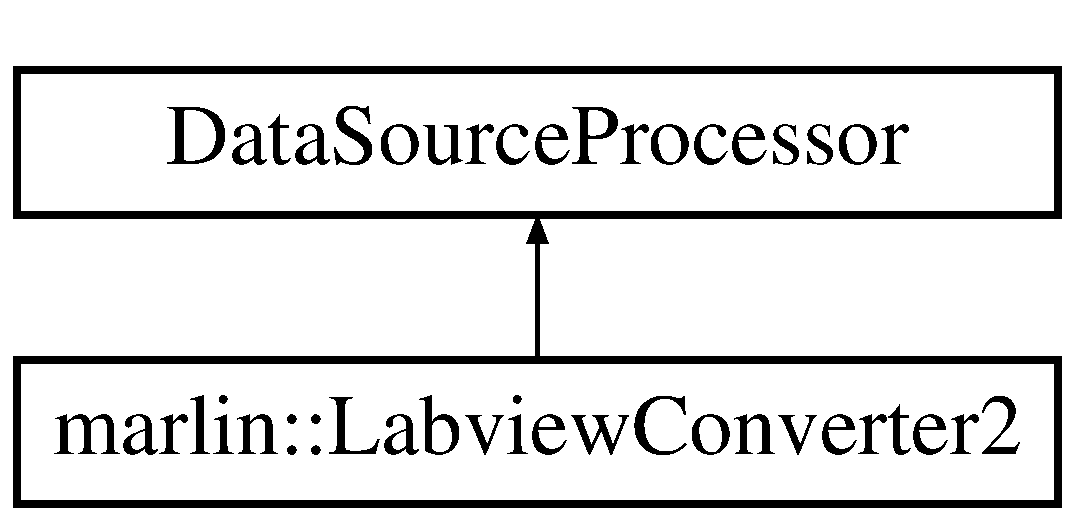
\includegraphics[height=2.000000cm]{classmarlin_1_1LabviewConverter2}
\end{center}
\end{figure}
\subsection*{Data Structures}
\begin{DoxyCompactItemize}
\item 
struct {\bf raw\-Data}
\begin{DoxyCompactList}\small\item\em The labview data format. \end{DoxyCompactList}\end{DoxyCompactItemize}
\subsection*{Public Member Functions}
\begin{DoxyCompactItemize}
\item 
virtual {\bf Labview\-Converter2} $\ast$ {\bf new\-Processor} ()\label{classmarlin_1_1LabviewConverter2_a675d56e8eeba4d2ad85e8ced3884b090}

\begin{DoxyCompactList}\small\item\em Implementation of new Processor returns pointer to processor. \end{DoxyCompactList}\item 
virtual void {\bf read\-Data\-Source} (int num\-Events)\label{classmarlin_1_1LabviewConverter2_a1548f59e1de895ed0d6ca0e749dd0261}

\begin{DoxyCompactList}\small\item\em Creates events with L\-C\-Genreal\-Object collections from the Labview input file and calls all active processors' process\-Event() and process\-Run\-Header Method. \end{DoxyCompactList}\item 
void {\bf write\-Slow\-Control} ()\label{classmarlin_1_1LabviewConverter2_a55ebf8a0b8a4d3227c106937dba96a39}

\begin{DoxyCompactList}\small\item\em work on slow control data, A\-S\-I\-C \end{DoxyCompactList}\item 
virtual void {\bf init} ()
\begin{DoxyCompactList}\small\item\em work on slow control data, Temperature \end{DoxyCompactList}\item 
virtual void {\bf end} ()\label{classmarlin_1_1LabviewConverter2_a3afe7b429e0851d276e01ead2115d848}

\begin{DoxyCompactList}\small\item\em end method \end{DoxyCompactList}\end{DoxyCompactItemize}
\subsection*{Protected Attributes}
\begin{DoxyCompactItemize}
\item 
std\-::string {\bf \-\_\-ofile}
\begin{DoxyCompactList}\small\item\em The string variable to access the data. \end{DoxyCompactList}\item 
std\-::string {\bf \-\_\-data}\label{classmarlin_1_1LabviewConverter2_a5256b6a520932eda9430b64bdc57d983}

\begin{DoxyCompactList}\small\item\em The string variable to access the data. \end{DoxyCompactList}\item 
int {\bf \-\_\-run\-Number}\label{classmarlin_1_1LabviewConverter2_a296e5632f4f412b507918e716198644a}

\begin{DoxyCompactList}\small\item\em The run number. \end{DoxyCompactList}\item 
int {\bf \-\_\-\-Slow\-Control\-Line\-Number}\label{classmarlin_1_1LabviewConverter2_ad4d497210ab5766096e996e31c6d4230}

\begin{DoxyCompactList}\small\item\em Slow control line number, H\-B\-U\-: 120, E\-P\-T\-: 1920. \end{DoxyCompactList}\item 
int {\bf \-\_\-\-H\-B\-U\-Number}
\begin{DoxyCompactList}\small\item\em The H\-B\-U number\-: H\-B\-U\-V\-I\-: 6; H\-B\-U\-V\-I\-: 7, H\-B\-U\-V\-I\-I\-I\-: 8, H\-B\-U\-I\-X\-: 9. \end{DoxyCompactList}\item 
int {\bf \-\_\-\-E\-P\-T\-Model\-Nr}\label{classmarlin_1_1LabviewConverter2_acb3e4506ca6a43017cfa26efa5170b99}

\begin{DoxyCompactList}\small\item\em The E\-P\-T model number\-: C\-E\-R\-N November testbeam E\-P\-T\-: 1. \end{DoxyCompactList}\item 
int {\bf n\-Corrupted\-Cycle}\label{classmarlin_1_1LabviewConverter2_a51f65918a12c7a77d03eba15a7d049cd}

\begin{DoxyCompactList}\small\item\em Counter for number of corrupted R\-O\-C. \end{DoxyCompactList}\item 
std\-::stringstream {\bf Slow\-Control}\label{classmarlin_1_1LabviewConverter2_ab042338dff0484ca2b443b04b548e190}

\begin{DoxyCompactList}\small\item\em Slow Control data block. \end{DoxyCompactList}\item 
std\-::string {\bf \-\_\-detector\-Type\-Name}\label{classmarlin_1_1LabviewConverter2_a856b33e1b7efb3a11e3e1f3d857edcc4}

\begin{DoxyCompactList}\small\item\em The string variable of the detector type name, A\-H\-C A\-E\-C. \end{DoxyCompactList}\end{DoxyCompactItemize}


\subsection{Detailed Description}
Processor for reading the A\-H\-C\-A\-L Labview asscii files. 

It processes the input data to create events with L\-C\-I\-O collections of the A\-H\-C\-A\-L Labview ascii output. Based on F. Gaede's Std\-Hep\-Reader to be found in the marlin package. \begin{DoxyAuthor}{Author}
\-: S. Lu (D\-E\-S\-Y Hamburg) 
\end{DoxyAuthor}
\begin{DoxyDate}{Date}
Aug 15 2012 
\end{DoxyDate}


Definition at line 18 of file Labview\-Converter2.\-hh.



\subsection{Member Function Documentation}
\index{marlin\-::\-Labview\-Converter2@{marlin\-::\-Labview\-Converter2}!init@{init}}
\index{init@{init}!marlin::LabviewConverter2@{marlin\-::\-Labview\-Converter2}}
\subsubsection[{init}]{\setlength{\rightskip}{0pt plus 5cm}void marlin\-::\-Labview\-Converter2\-::init (
\begin{DoxyParamCaption}
{}
\end{DoxyParamCaption}
)\hspace{0.3cm}{\ttfamily [virtual]}}\label{classmarlin_1_1LabviewConverter2_a69acbbef280d0aa78c058bc43bb7cc2d}


work on slow control data, Temperature 

init method 

Definition at line 66 of file Labview\-Converter2.\-cc.



References n\-Corrupted\-Cycle.



\subsection{Field Documentation}
\index{marlin\-::\-Labview\-Converter2@{marlin\-::\-Labview\-Converter2}!\-\_\-\-H\-B\-U\-Number@{\-\_\-\-H\-B\-U\-Number}}
\index{\-\_\-\-H\-B\-U\-Number@{\-\_\-\-H\-B\-U\-Number}!marlin::LabviewConverter2@{marlin\-::\-Labview\-Converter2}}
\subsubsection[{\-\_\-\-H\-B\-U\-Number}]{\setlength{\rightskip}{0pt plus 5cm}int marlin\-::\-Labview\-Converter2\-::\-\_\-\-H\-B\-U\-Number\hspace{0.3cm}{\ttfamily [protected]}}\label{classmarlin_1_1LabviewConverter2_a8dc9c62b6c335f9af82b17b00b7c6c1b}


The H\-B\-U number\-: H\-B\-U\-V\-I\-: 6; H\-B\-U\-V\-I\-: 7, H\-B\-U\-V\-I\-I\-I\-: 8, H\-B\-U\-I\-X\-: 9. 



Definition at line 66 of file Labview\-Converter2.\-hh.

\index{marlin\-::\-Labview\-Converter2@{marlin\-::\-Labview\-Converter2}!\-\_\-ofile@{\-\_\-ofile}}
\index{\-\_\-ofile@{\-\_\-ofile}!marlin::LabviewConverter2@{marlin\-::\-Labview\-Converter2}}
\subsubsection[{\-\_\-ofile}]{\setlength{\rightskip}{0pt plus 5cm}std\-::string marlin\-::\-Labview\-Converter2\-::\-\_\-ofile\hspace{0.3cm}{\ttfamily [protected]}}\label{classmarlin_1_1LabviewConverter2_a71f598537b02b4a46c1c2622dbac8d9e}


The string variable to access the data. 

Requires \char`\"{}yourpath/\-Run\char`\"{} 

Definition at line 53 of file Labview\-Converter2.\-hh.



The documentation for this class was generated from the following files\-:\begin{DoxyCompactItemize}
\item 
Labview\-Converter2.\-hh\item 
Labview\-Converter2.\-cc\end{DoxyCompactItemize}

\section{L\-Converter Class Reference}
\label{classLConverter}\index{L\-Converter@{L\-Converter}}
\subsection*{Public Member Functions}
\begin{DoxyCompactItemize}
\item 
std\-::vector$<$ int $>$ {\bfseries Get\-Bunch\-X\-I\-D} () const \label{classLConverter_aa36cabb750e60dab0c27a8868fbf822f}

\item 
std\-::vector$<$ int $>$ {\bfseries Get\-Cycle\-Nr} () const \label{classLConverter_ade0160100df41b58edb54a6cccf265f2}

\item 
std\-::vector$<$ int $>$ {\bfseries Get\-Chip\-I\-D} () const \label{classLConverter_a7e258458a690e3f969078eb0e2b25550}

\item 
std\-::vector$<$ int $>$ {\bfseries Get\-A\-S\-I\-C\-Nr} () const \label{classLConverter_afd5677457e034b1314b16c12cb379a1e}

\item 
std\-::vector$<$ int $>$ {\bfseries Get\-Evt\-Nr} () const \label{classLConverter_a75d43fbe9aeb66f852a72ef5b3acdac3}

\item 
std\-::vector$<$ int $>$ {\bfseries Get\-Channel} () const \label{classLConverter_a421bc622c868a9acb10cbf371d967619}

\item 
std\-::vector$<$ int $>$ {\bfseries Get\-T\-D\-C} () const \label{classLConverter_a6b3fb44f0f5dd2aec1abea2b9c6b11a5}

\item 
std\-::vector$<$ int $>$ {\bfseries Get\-A\-D\-C} () const \label{classLConverter_a281711127b23f444867fd96ab112cec7}

\item 
std\-::vector$<$ int $>$ {\bfseries Get\-X\-Pos} () const \label{classLConverter_aa984a603c6c7dd60c412818d580d4a1e}

\item 
std\-::vector$<$ int $>$ {\bfseries Get\-Y\-Pos} () const \label{classLConverter_ab7e4941672713e1e654d964a2983e619}

\item 
std\-::vector$<$ int $>$ {\bfseries Get\-Hit\-Bit} () const \label{classLConverter_a373903e1cda893fccbc8a0a64581cedf}

\item 
std\-::vector$<$ int $>$ {\bfseries Get\-Gain\-Bit} () const \label{classLConverter_a5e61fac60253d34fa40a9c5442a13196}

\item 
void {\bfseries Set\-Bunch\-X\-I\-D} (int Bunch\-X\-I\-D)\label{classLConverter_a05a8cef4b9c87f720261fc52cce1e193}

\item 
void {\bfseries Set\-Cycle\-Nr} (int Cycle\-Nr)\label{classLConverter_a7efeeb526c6db39ff43a017bb74b29e0}

\item 
void {\bfseries Set\-Chip\-I\-D} (int Chip\-I\-D)\label{classLConverter_a37f140c2b9055799ee6a82cc4d73c44e}

\item 
void {\bfseries Set\-A\-S\-I\-C\-Nr} (int A\-S\-I\-C\-Nr)\label{classLConverter_acfc4cc61fc627016acaf883f4d0046d4}

\item 
void {\bfseries Set\-Evt\-Nr} (int Evt\-Nr)\label{classLConverter_ac5115b177d290824b2a787b9e068fc19}

\item 
void {\bfseries Set\-Channel} (int Channel)\label{classLConverter_a340a2d351e2fdadccaf9dd197f50237c}

\item 
void {\bfseries Set\-T\-D\-C} (int T\-D\-C)\label{classLConverter_a08fa1525b279272c5c5e54b63d1cb201}

\item 
void {\bfseries Set\-A\-D\-C} (int A\-D\-C)\label{classLConverter_ac5bd4c6306a2cee6a935e973058a905a}

\item 
void {\bfseries Set\-X\-Pos} (int X\-Pos)\label{classLConverter_a6971660f486140f26227ceaf7a8ce09a}

\item 
void {\bfseries Set\-Y\-Pos} (int Y\-Pos)\label{classLConverter_adc5fee91ab6526179b186ad11ab25c7e}

\item 
void {\bfseries Set\-Hit\-Bit} (int Hit\-Bit)\label{classLConverter_aaa94bc9bb1609136b6fd81523649c53c}

\item 
void {\bfseries Set\-Gain\-Bit} (int Gain\-Bit)\label{classLConverter_a8c8d34fb8da1b09a171ca7ab345aaaaf}

\item 
void {\bfseries Set\-L\-Converter} (int Data[$\,$])\label{classLConverter_a180d5e6b80a72eeab6ab0cb090d0c740}

\item 
void {\bfseries Clear} (void)\label{classLConverter_a9251a44afb49f1215749cb2e409beb6d}

\item 
void {\bfseries Erase} (int i)\label{classLConverter_a4966e1ffc3dd538c66336cf8d29fea22}

\item 
void {\bfseries Reverse} (void)\label{classLConverter_a308aa32941ea7dadb65354958ed26b6b}

\item 
void {\bfseries swap\-Bunch\-X\-I\-D} (void)\label{classLConverter_ac018aa0de8c404849ac58ba98232a7b2}

\item 
void {\bfseries Swap\-Evt\-Nr} (void)\label{classLConverter_a8d23856e6cd95500295bfc4f7decf252}

\item 
void {\bfseries Print\-Parameters} (int i)\label{classLConverter_adf37266688bb924ffe3ca72787115a17}

\item 
void {\bfseries Print\-Parameters\-Label} ()\label{classLConverter_a0ca415c8251400c2db08b8efeaeda600}

\end{DoxyCompactItemize}
\subsection*{Private Attributes}
\begin{DoxyCompactItemize}
\item 
std\-::vector$<$ int $>$ {\bfseries \-\_\-data\-Bunch\-X\-I\-D}\label{classLConverter_a2f5f56717c60559527081359819d0258}

\item 
std\-::vector$<$ int $>$ {\bfseries \-\_\-data\-Cycle\-Nr}\label{classLConverter_acc1467c848aa450844a9a06951199026}

\item 
std\-::vector$<$ int $>$ {\bfseries \-\_\-data\-Chip\-I\-D}\label{classLConverter_a887aa94f82e828880724d5ba748ddd77}

\item 
std\-::vector$<$ int $>$ {\bfseries \-\_\-data\-A\-S\-I\-C\-Nr}\label{classLConverter_a2499df9981bc1ace21338afb6d062c9e}

\item 
std\-::vector$<$ int $>$ {\bfseries \-\_\-data\-Evt\-Nr}\label{classLConverter_a6cdcb023717210662d77fcb5290d691e}

\item 
std\-::vector$<$ int $>$ {\bfseries \-\_\-data\-Channel}\label{classLConverter_ae8d815dfef08c8a3051947f91087dc43}

\item 
std\-::vector$<$ int $>$ {\bfseries \-\_\-data\-T\-D\-C}\label{classLConverter_abc01471700894cc45f54911add87be8a}

\item 
std\-::vector$<$ int $>$ {\bfseries \-\_\-data\-A\-D\-C}\label{classLConverter_aed17939cbd31aa3d610d603d75237efc}

\item 
std\-::vector$<$ int $>$ {\bfseries \-\_\-data\-X\-Pos}\label{classLConverter_a8c5903b40e0d932d78a22ad6b6eb1533}

\item 
std\-::vector$<$ int $>$ {\bfseries \-\_\-data\-Y\-Pos}\label{classLConverter_a0da4582926094b15372b9edb7acbe178}

\item 
std\-::vector$<$ int $>$ {\bfseries \-\_\-data\-Hit\-Bit}\label{classLConverter_a60a52921a0dcc933e3da1a4be4d7e237}

\item 
std\-::vector$<$ int $>$ {\bfseries \-\_\-data\-Gain\-Bit}\label{classLConverter_a84103da9f656d6327a35a3f80e37cdf1}

\end{DoxyCompactItemize}


\subsection{Detailed Description}


Definition at line 14 of file L\-Converter.\-hh.



The documentation for this class was generated from the following file\-:\begin{DoxyCompactItemize}
\item 
L\-Converter.\-hh\end{DoxyCompactItemize}

\section{C\-A\-L\-I\-C\-E\-:\-:L\-D\-A\-Block Class Reference}
\label{classCALICE_1_1LDABlock}\index{C\-A\-L\-I\-C\-E\-::\-L\-D\-A\-Block@{C\-A\-L\-I\-C\-E\-::\-L\-D\-A\-Block}}


Class for the S\-L\-C\-I\-O E\-U\-D\-A\-Q B\-I\-F Data as acquired by the E\-U\-D\-A\-Q system.  




{\ttfamily \#include $<$L\-D\-A\-Block.\-hh$>$}

Inheritance diagram for C\-A\-L\-I\-C\-E\-:\-:L\-D\-A\-Block\-:\begin{figure}[H]
\begin{center}
\leavevmode
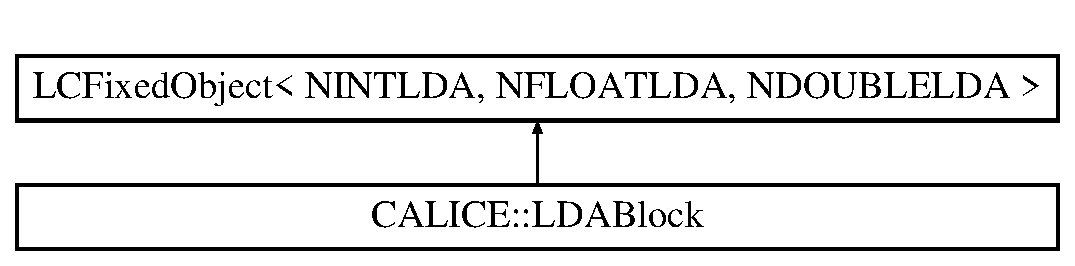
\includegraphics[height=2.000000cm]{classCALICE_1_1LDABlock}
\end{center}
\end{figure}
\subsection*{Public Member Functions}
\begin{DoxyCompactItemize}
\item 
{\bf L\-D\-A\-Block} ()\label{classCALICE_1_1LDABlock_a9ebbc6dc0b81b6e1a262a0eacbddba6f}

\begin{DoxyCompactList}\small\item\em Constructor. \end{DoxyCompactList}\item 
{\bfseries L\-D\-A\-Block} (L\-C\-Object $\ast$obj)\label{classCALICE_1_1LDABlock_aa4951561a8f9621112ccef2cd9460b57}

\item 
{\bf L\-D\-A\-Block} (unsigned long long int Start\-Acq, unsigned long long int Stop\-Acq, unsigned long int Trigger\-Time\-Low, unsigned long int Trigger\-Time\-High)\label{classCALICE_1_1LDABlock_ad6d90f79de9f214f6992cd5c730ecb9c}

\begin{DoxyCompactList}\small\item\em Convenient constructor. \end{DoxyCompactList}\item 
virtual {\bf $\sim$\-L\-D\-A\-Block} ()\label{classCALICE_1_1LDABlock_af30bb970cb30721583ecdb540d191854}

\begin{DoxyCompactList}\small\item\em Destructor. \end{DoxyCompactList}\item 
void {\bf print} (std\-::ostream \&os, int)\label{classCALICE_1_1LDABlock_a18b09b2d2ce5e3ae3f78cd86756fb40e}

\begin{DoxyCompactList}\small\item\em Convenient print method. \end{DoxyCompactList}\item 
void {\bfseries set\-Start\-Acq} (unsigned long long int Start\-Acq)\label{classCALICE_1_1LDABlock_ae2ae1f21a4bccff7f7d1a7f39f485725}

\item 
void {\bfseries set\-Stop\-Acq} (unsigned long long int Stop\-Acq)\label{classCALICE_1_1LDABlock_a00fc7b0396672e6bf7fef63ae354f47d}

\item 
void {\bf set\-Trigger\-Time\-Low} (unsigned long int Trigger\-Time\-Low)\label{classCALICE_1_1LDABlock_ad0370f93ee3602a5251515f8f98e5382}

\begin{DoxyCompactList}\small\item\em Set Time of the L\-D\-A Trigger. \end{DoxyCompactList}\item 
void {\bfseries set\-Trigger\-Time\-High} (unsigned long int Trigger\-Time\-High)\label{classCALICE_1_1LDABlock_aa050d4415f0b306dff6fba5ae6217654}

\item 
unsigned long long int {\bfseries get\-Start\-Acq} () const \label{classCALICE_1_1LDABlock_afe2c965b42ed1a3d07ac5a5c373c9aff}

\item 
unsigned long long int {\bfseries get\-Stop\-Acq} () const \label{classCALICE_1_1LDABlock_a1aec54f5a7fd69296291eeb8a53b4685}

\item 
unsigned long int {\bf get\-Trigger\-Time\-Low} () const \label{classCALICE_1_1LDABlock_a52f34a278f3b9d28555213a401e93a27}

\begin{DoxyCompactList}\small\item\em Get Time of the L\-D\-A Trigger. \end{DoxyCompactList}\item 
unsigned long int {\bfseries get\-Trigger\-Time\-High} () const \label{classCALICE_1_1LDABlock_a11f4e660c66bf364823b5759698619a9}

\item 
const std\-::string {\bf get\-Type\-Name} () const \label{classCALICE_1_1LDABlock_a6d66f30a375e65f742af053a0e21d244}

\begin{DoxyCompactList}\small\item\em Return the type of the class. \end{DoxyCompactList}\item 
const std\-::string {\bf get\-Data\-Description} () const \label{classCALICE_1_1LDABlock_a579cbbe48f3d7b65f995461df745990e}

\begin{DoxyCompactList}\small\item\em Return a brief description of the data members. \end{DoxyCompactList}\end{DoxyCompactItemize}


\subsection{Detailed Description}
Class for the S\-L\-C\-I\-O E\-U\-D\-A\-Q B\-I\-F Data as acquired by the E\-U\-D\-A\-Q system. 

\begin{DoxyAuthor}{Author}
E.\-Brianne @ D\-E\-S\-Y Hamburg 
\end{DoxyAuthor}
\begin{DoxyDate}{Date}
May 2016 Created for 2016 testbeams E\-U\-D\-A\-Q data format. 
\end{DoxyDate}


Definition at line 23 of file L\-D\-A\-Block.\-hh.



The documentation for this class was generated from the following file\-:\begin{DoxyCompactItemize}
\item 
L\-D\-A\-Block.\-hh\end{DoxyCompactItemize}

\section{Line\-Fitter Class Reference}
\label{classLineFitter}\index{Line\-Fitter@{Line\-Fitter}}
\subsection*{Public Member Functions}
\begin{DoxyCompactItemize}
\item 
{\bfseries Line\-Fitter} (std\-::vector$<$ float $>$ x, std\-::vector$<$ float $>$ y, std\-::vector$<$ float $>$ sigma\-\_\-y)\label{classLineFitter_afa54506230c2b69789d8405155b872e2}

\item 
void {\bfseries add\-Point} (float x, float y, float sigma\-\_\-y)\label{classLineFitter_a6c8d60770b882a3dfa7f497c6357e8c6}

\item 
void {\bfseries clear} ()\label{classLineFitter_abb9dcd9e88541d736c8e7d00e7760c98}

\item 
void {\bfseries fit} ()\label{classLineFitter_a0c8db2f9d3b0c0247abf09cb47b4194c}

\item 
bool {\bfseries converged} ()\label{classLineFitter_a2784cf556129b2bff9f4efb65dc577e4}

\item 
float {\bfseries get\-M} ()\label{classLineFitter_a06e09c67148d7e1dd5d6685ab0270988}

\item 
float {\bfseries get\-M\-Error} ()\label{classLineFitter_a21693b557fa869c24d7bdd4e67e9e2cf}

\item 
float {\bfseries get\-B} ()\label{classLineFitter_abda6c35013a6d0a0eed77320aff46e31}

\item 
float {\bfseries get\-B\-Error} ()\label{classLineFitter_aa2b281f268cd91c78beed523a36973a3}

\item 
float {\bfseries get\-M\-B\-Covariance} ()\label{classLineFitter_a5fe74da585902fbf1fb41698be2c05c2}

\item 
float {\bfseries eval} (float x)\label{classLineFitter_abf22cdfdd40160cfc60444a450bc069f}

\item 
float {\bfseries eval\-Error} (float x)\label{classLineFitter_a25e0bff99cfa6099550482b1af674d4d}

\item 
int {\bfseries Get\-N\-D\-F} ()\label{classLineFitter_a868ec66a5b8d1e0ff4255648e7d3d1dc}

\item 
float {\bfseries Get\-Chisquare} ()\label{classLineFitter_ad5366bef4af95ea825a9637b296844fa}

\end{DoxyCompactItemize}
\subsection*{Private Attributes}
\begin{DoxyCompactItemize}
\item 
std\-::vector$<$ float $>$ {\bfseries \-\_\-x}\label{classLineFitter_ae43423c2f6fe5ef3b9c2418ec231a570}

\item 
std\-::vector$<$ float $>$ {\bfseries \-\_\-y}\label{classLineFitter_adc9dca456fddfff7737eb7711319d156}

\item 
std\-::vector$<$ float $>$ {\bfseries \-\_\-sigma\-\_\-y}\label{classLineFitter_a255fc2f0df061e83fca7937458122ee1}

\item 
float {\bfseries \-\_\-\-S}\label{classLineFitter_a005727d31fe2adb0ca0fb0a5c8f5b07d}

\item 
float {\bfseries \-\_\-\-S\-\_\-x}\label{classLineFitter_a1c4328b5bfae8c57c2e644638125a71a}

\item 
float {\bfseries \-\_\-\-S\-\_\-xx}\label{classLineFitter_acd98cdf41dfb567e8cea616c88263cea}

\item 
float {\bfseries \-\_\-\-S\-\_\-xy}\label{classLineFitter_a278f1df0817c39933b3cab33b66532f8}

\item 
float {\bfseries \-\_\-\-S\-\_\-y}\label{classLineFitter_aeeb3cef703dc326c9ab58cc2c13a0bae}

\item 
float {\bfseries \-\_\-\-Delta}\label{classLineFitter_a1620b20e524128ea6eef19010bb82fe2}

\end{DoxyCompactItemize}


\subsection{Detailed Description}


Definition at line 5 of file Line\-Fitter.\-hh.



The documentation for this class was generated from the following files\-:\begin{DoxyCompactItemize}
\item 
Line\-Fitter.\-hh\item 
Line\-Fitter.\-cc\end{DoxyCompactItemize}

\section{C\-A\-L\-I\-C\-E\-:\-:E\-U\-D\-A\-Q\-Event\-Builder\-:\-:raw\-Data Struct Reference}
\label{structCALICE_1_1EUDAQEventBuilder_1_1rawData}\index{C\-A\-L\-I\-C\-E\-::\-E\-U\-D\-A\-Q\-Event\-Builder\-::raw\-Data@{C\-A\-L\-I\-C\-E\-::\-E\-U\-D\-A\-Q\-Event\-Builder\-::raw\-Data}}


The slcio data format.  




{\ttfamily \#include $<$E\-U\-D\-A\-Q\-Event\-Builder.\-hh$>$}

\subsection*{Data Fields}
\begin{DoxyCompactItemize}
\item 
int {\bfseries i\-Cy\-Nr}\label{structCALICE_1_1EUDAQEventBuilder_1_1rawData_a006628d4355eff92eedfa9a6cd750c1f}

\item 
int {\bfseries i\-Bx\-I\-D}\label{structCALICE_1_1EUDAQEventBuilder_1_1rawData_a2212434bb5aaf722fb96d9c40c7b4d51}

\item 
int {\bfseries i\-Cp\-I\-D}\label{structCALICE_1_1EUDAQEventBuilder_1_1rawData_aaf2e66f34599ecd9a7ec6eba19e7946e}

\item 
int {\bfseries i\-Ev\-Nr}\label{structCALICE_1_1EUDAQEventBuilder_1_1rawData_ad098fe7746808f4d3401d1c2a40f646f}

\item 
int {\bfseries i\-Chan}\label{structCALICE_1_1EUDAQEventBuilder_1_1rawData_a622d82b2d99fe835f2e587d3f7e20724}

\item 
int {\bfseries i\-T\-D\-C}\label{structCALICE_1_1EUDAQEventBuilder_1_1rawData_abad5c342509389ba287acc4e5a326276}

\item 
int {\bfseries i\-A\-D\-C}\label{structCALICE_1_1EUDAQEventBuilder_1_1rawData_ad2301901a9a551c242b2d25e22654b4d}

\item 
int {\bfseries i\-H\-Bit}\label{structCALICE_1_1EUDAQEventBuilder_1_1rawData_ae4b96f164ea2de6026eb4c1273da263a}

\item 
int {\bfseries i\-G\-Bit}\label{structCALICE_1_1EUDAQEventBuilder_1_1rawData_a3f8979de8030b4108bd673971db3104f}

\end{DoxyCompactItemize}


\subsection{Detailed Description}
The slcio data format. 

Definition at line 69 of file E\-U\-D\-A\-Q\-Event\-Builder.\-hh.



The documentation for this struct was generated from the following file\-:\begin{DoxyCompactItemize}
\item 
E\-U\-D\-A\-Q\-Event\-Builder.\-hh\end{DoxyCompactItemize}

\section{C\-A\-L\-I\-C\-E\-:\-:E\-U\-D\-A\-Q\-Event\-Builder2018\-\_\-cosmics\-:\-:raw\-Data Struct Reference}
\label{structCALICE_1_1EUDAQEventBuilder2018__cosmics_1_1rawData}\index{C\-A\-L\-I\-C\-E\-::\-E\-U\-D\-A\-Q\-Event\-Builder2018\-\_\-cosmics\-::raw\-Data@{C\-A\-L\-I\-C\-E\-::\-E\-U\-D\-A\-Q\-Event\-Builder2018\-\_\-cosmics\-::raw\-Data}}


The slcio data format.  




{\ttfamily \#include $<$E\-U\-D\-A\-Q\-Event\-Builder2018\-\_\-cosmics.\-hh$>$}

\subsection*{Data Fields}
\begin{DoxyCompactItemize}
\item 
int {\bfseries i\-Cy\-Nr}\label{structCALICE_1_1EUDAQEventBuilder2018__cosmics_1_1rawData_a26731a4573683d1762864b79d44537a6}

\item 
int {\bfseries i\-Bx\-I\-D}\label{structCALICE_1_1EUDAQEventBuilder2018__cosmics_1_1rawData_a52336f10191ed552d55380e3e7f33b0e}

\item 
int {\bfseries i\-Cp\-I\-D}\label{structCALICE_1_1EUDAQEventBuilder2018__cosmics_1_1rawData_adce6b5abf72e5bcbcff7908fb534fb04}

\item 
int {\bfseries i\-Ev\-Nr}\label{structCALICE_1_1EUDAQEventBuilder2018__cosmics_1_1rawData_a543148e3707cb5d6c48baa9da2cd850e}

\item 
int {\bfseries i\-Chan}\label{structCALICE_1_1EUDAQEventBuilder2018__cosmics_1_1rawData_a3e990facb75c9f8d0857340554fc50a8}

\item 
int {\bfseries i\-T\-D\-C}\label{structCALICE_1_1EUDAQEventBuilder2018__cosmics_1_1rawData_aa9c7381ef8c72646d4ddcc8bcc6c9a3d}

\item 
int {\bfseries i\-A\-D\-C}\label{structCALICE_1_1EUDAQEventBuilder2018__cosmics_1_1rawData_ac047e72373c5ddb9cb99bc4db84658d2}

\item 
int {\bfseries i\-H\-Bit}\label{structCALICE_1_1EUDAQEventBuilder2018__cosmics_1_1rawData_a98b7fbca150160baa217e8671c224a8a}

\item 
int {\bfseries i\-G\-Bit}\label{structCALICE_1_1EUDAQEventBuilder2018__cosmics_1_1rawData_aee2745acdc1816d126ac2c4baa613a60}

\item 
int {\bfseries i\-H\-Bit2}\label{structCALICE_1_1EUDAQEventBuilder2018__cosmics_1_1rawData_a273555c51f257a133ef2c88955ae5900}

\item 
int {\bfseries i\-G\-Bit2}\label{structCALICE_1_1EUDAQEventBuilder2018__cosmics_1_1rawData_af9c83e421af8b8b7c21dfa2382a0c7db}

\end{DoxyCompactItemize}


\subsection{Detailed Description}
The slcio data format. 

Definition at line 75 of file E\-U\-D\-A\-Q\-Event\-Builder2018\-\_\-cosmics.\-hh.



The documentation for this struct was generated from the following file\-:\begin{DoxyCompactItemize}
\item 
E\-U\-D\-A\-Q\-Event\-Builder2018\-\_\-cosmics.\-hh\end{DoxyCompactItemize}

\section{C\-A\-L\-I\-C\-E\-:\-:E\-U\-D\-A\-Q\-Event\-Builder2016\-\_\-wo\-B\-I\-F\-:\-:raw\-Data Struct Reference}
\label{structCALICE_1_1EUDAQEventBuilder2016__woBIF_1_1rawData}\index{C\-A\-L\-I\-C\-E\-::\-E\-U\-D\-A\-Q\-Event\-Builder2016\-\_\-wo\-B\-I\-F\-::raw\-Data@{C\-A\-L\-I\-C\-E\-::\-E\-U\-D\-A\-Q\-Event\-Builder2016\-\_\-wo\-B\-I\-F\-::raw\-Data}}


The slcio data format.  




{\ttfamily \#include $<$E\-U\-D\-A\-Q\-Event\-Builder2016\-\_\-wo\-B\-I\-F.\-hh$>$}

\subsection*{Data Fields}
\begin{DoxyCompactItemize}
\item 
int {\bfseries i\-Cy\-Nr}\label{structCALICE_1_1EUDAQEventBuilder2016__woBIF_1_1rawData_a6a64e70bd4342445819aafaff55cde96}

\item 
int {\bfseries i\-Bx\-I\-D}\label{structCALICE_1_1EUDAQEventBuilder2016__woBIF_1_1rawData_a203dc50d5e7cf14bb33a35205e662a01}

\item 
int {\bfseries i\-Cp\-I\-D}\label{structCALICE_1_1EUDAQEventBuilder2016__woBIF_1_1rawData_af2436c619f2ae2ccb7058acfcbb7847d}

\item 
int {\bfseries i\-Ev\-Nr}\label{structCALICE_1_1EUDAQEventBuilder2016__woBIF_1_1rawData_aab3c629ab26381d91723fe53e78f6b0a}

\item 
int {\bfseries i\-Chan}\label{structCALICE_1_1EUDAQEventBuilder2016__woBIF_1_1rawData_aedadfc60836e09c517ed1317a11326d5}

\item 
int {\bfseries i\-T\-D\-C}\label{structCALICE_1_1EUDAQEventBuilder2016__woBIF_1_1rawData_ad0a510cad8868942619ca43d89aa8e3e}

\item 
int {\bfseries i\-A\-D\-C}\label{structCALICE_1_1EUDAQEventBuilder2016__woBIF_1_1rawData_afbc9688928feced75387643ab18cbada}

\item 
int {\bfseries i\-H\-Bit}\label{structCALICE_1_1EUDAQEventBuilder2016__woBIF_1_1rawData_a7af0294a0a633f9b32c10888f90ac613}

\item 
int {\bfseries i\-G\-Bit}\label{structCALICE_1_1EUDAQEventBuilder2016__woBIF_1_1rawData_ad75449bd3f2e3d2e4ccac166e51fac5b}

\item 
int {\bfseries i\-H\-Bit2}\label{structCALICE_1_1EUDAQEventBuilder2016__woBIF_1_1rawData_a2f899ab0ba3d0a50f277a7843893a2a9}

\item 
int {\bfseries i\-G\-Bit2}\label{structCALICE_1_1EUDAQEventBuilder2016__woBIF_1_1rawData_a82e6c705987f3f1e12c212c541c9d78a}

\end{DoxyCompactItemize}


\subsection{Detailed Description}
The slcio data format. 

Definition at line 75 of file E\-U\-D\-A\-Q\-Event\-Builder2016\-\_\-wo\-B\-I\-F.\-hh.



The documentation for this struct was generated from the following file\-:\begin{DoxyCompactItemize}
\item 
E\-U\-D\-A\-Q\-Event\-Builder2016\-\_\-wo\-B\-I\-F.\-hh\end{DoxyCompactItemize}

\section{marlin\-:\-:Labview\-Converter2\-:\-:raw\-Data Struct Reference}
\label{structmarlin_1_1LabviewConverter2_1_1rawData}\index{marlin\-::\-Labview\-Converter2\-::raw\-Data@{marlin\-::\-Labview\-Converter2\-::raw\-Data}}


The labview data format.  




{\ttfamily \#include $<$Labview\-Converter2.\-hh$>$}

\subsection*{Data Fields}
\begin{DoxyCompactItemize}
\item 
int {\bfseries i\-Cy\-Nr}\label{structmarlin_1_1LabviewConverter2_1_1rawData_a03006803e0b5b2da5820d8bc95b25821}

\item 
int {\bfseries i\-Bx\-I\-D}\label{structmarlin_1_1LabviewConverter2_1_1rawData_a18813688dc645068904762d7179caabf}

\item 
int {\bfseries i\-Cp\-I\-D}\label{structmarlin_1_1LabviewConverter2_1_1rawData_a4b6d90d46ac4234bb39db626efe25b90}

\item 
int {\bfseries i\-Ev\-Nr}\label{structmarlin_1_1LabviewConverter2_1_1rawData_a4e4d521b9951a3a093add42abe718d24}

\item 
int {\bfseries i\-Chan}\label{structmarlin_1_1LabviewConverter2_1_1rawData_a2c95f1ea0b28bde1aa11fa0c17831e33}

\item 
int {\bfseries i\-T\-D\-C}\label{structmarlin_1_1LabviewConverter2_1_1rawData_a70f867c80e05e01037317f08d09341fb}

\item 
int {\bfseries i\-A\-D\-C}\label{structmarlin_1_1LabviewConverter2_1_1rawData_a0a42ca5b0eb49a252c6b6fbc565978a4}

\item 
int {\bfseries i\-H\-Bit}\label{structmarlin_1_1LabviewConverter2_1_1rawData_a82258aad93b77ba908e7b751d59088a1}

\item 
int {\bfseries i\-G\-Bit}\label{structmarlin_1_1LabviewConverter2_1_1rawData_ae932bf4a10f7064fbd36b823eca20f6e}

\end{DoxyCompactItemize}


\subsection{Detailed Description}
The labview data format. 

Definition at line 84 of file Labview\-Converter2.\-hh.



The documentation for this struct was generated from the following file\-:\begin{DoxyCompactItemize}
\item 
Labview\-Converter2.\-hh\end{DoxyCompactItemize}

\section{C\-A\-L\-I\-C\-E\-:\-:E\-U\-D\-A\-Q\-Event\-Builder2016\-\_\-wo\-B\-I\-F\-:\-:raw\-Data2016 Struct Reference}
\label{structCALICE_1_1EUDAQEventBuilder2016__woBIF_1_1rawData2016}\index{C\-A\-L\-I\-C\-E\-::\-E\-U\-D\-A\-Q\-Event\-Builder2016\-\_\-wo\-B\-I\-F\-::raw\-Data2016@{C\-A\-L\-I\-C\-E\-::\-E\-U\-D\-A\-Q\-Event\-Builder2016\-\_\-wo\-B\-I\-F\-::raw\-Data2016}}


The slcio data format.  




{\ttfamily \#include $<$E\-U\-D\-A\-Q\-Event\-Builder2016\-\_\-wo\-B\-I\-F.\-hh$>$}

\subsection*{Data Fields}
\begin{DoxyCompactItemize}
\item 
int {\bfseries i\-Cycle\-Nr}\label{structCALICE_1_1EUDAQEventBuilder2016__woBIF_1_1rawData2016_a60345bf308d7a9c2aea61058bbcae186}

\item 
int {\bfseries i\-Bx\-I\-D}\label{structCALICE_1_1EUDAQEventBuilder2016__woBIF_1_1rawData2016_a3b0a013af57afc6c66d51544912accdd}

\item 
int {\bfseries i\-Ev\-Nr}\label{structCALICE_1_1EUDAQEventBuilder2016__woBIF_1_1rawData2016_acaf440a212bc84243d58377081b964bd}

\item 
int {\bfseries i\-Cp\-I\-D}\label{structCALICE_1_1EUDAQEventBuilder2016__woBIF_1_1rawData2016_ae22ff69e72deb92b788c4f92a74fa9cd}

\item 
int {\bfseries i\-N\-Chan}\label{structCALICE_1_1EUDAQEventBuilder2016__woBIF_1_1rawData2016_afd98d07285d886e0659297eb7b6679cf}

\item 
std\-::vector$<$ int $>$ {\bfseries i\-T\-D\-C}\label{structCALICE_1_1EUDAQEventBuilder2016__woBIF_1_1rawData2016_aeee048eee49339800053b4b30f363486}

\item 
std\-::vector$<$ int $>$ {\bfseries i\-A\-D\-C}\label{structCALICE_1_1EUDAQEventBuilder2016__woBIF_1_1rawData2016_a2d70d493fb1d0ce9cec3a3f5679e4c42}

\end{DoxyCompactItemize}


\subsection{Detailed Description}
The slcio data format. 

Definition at line 91 of file E\-U\-D\-A\-Q\-Event\-Builder2016\-\_\-wo\-B\-I\-F.\-hh.



The documentation for this struct was generated from the following file\-:\begin{DoxyCompactItemize}
\item 
E\-U\-D\-A\-Q\-Event\-Builder2016\-\_\-wo\-B\-I\-F.\-hh\end{DoxyCompactItemize}

\section{C\-A\-L\-I\-C\-E\-:\-:E\-U\-D\-A\-Q\-Event\-Builder2018\-\_\-cosmics\-:\-:raw\-Data2016 Struct Reference}
\label{structCALICE_1_1EUDAQEventBuilder2018__cosmics_1_1rawData2016}\index{C\-A\-L\-I\-C\-E\-::\-E\-U\-D\-A\-Q\-Event\-Builder2018\-\_\-cosmics\-::raw\-Data2016@{C\-A\-L\-I\-C\-E\-::\-E\-U\-D\-A\-Q\-Event\-Builder2018\-\_\-cosmics\-::raw\-Data2016}}


The slcio data format.  




{\ttfamily \#include $<$E\-U\-D\-A\-Q\-Event\-Builder2018\-\_\-cosmics.\-hh$>$}

\subsection*{Data Fields}
\begin{DoxyCompactItemize}
\item 
int {\bfseries i\-Cycle\-Nr}\label{structCALICE_1_1EUDAQEventBuilder2018__cosmics_1_1rawData2016_abd9be451984a46dbcdad0a5db2ee49bc}

\item 
int {\bfseries i\-Bx\-I\-D}\label{structCALICE_1_1EUDAQEventBuilder2018__cosmics_1_1rawData2016_a61590df6b9ae8889c929b45cf747014e}

\item 
int {\bfseries i\-Ev\-Nr}\label{structCALICE_1_1EUDAQEventBuilder2018__cosmics_1_1rawData2016_ace73806ad02a0150af959d00595da619}

\item 
int {\bfseries i\-Cp\-I\-D}\label{structCALICE_1_1EUDAQEventBuilder2018__cosmics_1_1rawData2016_af25e5c9e45f0eec3637e2132c82350c3}

\item 
int {\bfseries i\-N\-Chan}\label{structCALICE_1_1EUDAQEventBuilder2018__cosmics_1_1rawData2016_a61c776c9884b89ea3da2abd3bf27d8ae}

\item 
std\-::vector$<$ int $>$ {\bfseries i\-T\-D\-C}\label{structCALICE_1_1EUDAQEventBuilder2018__cosmics_1_1rawData2016_a21ac10d5a303008b3c2667e5a834ec59}

\item 
std\-::vector$<$ int $>$ {\bfseries i\-A\-D\-C}\label{structCALICE_1_1EUDAQEventBuilder2018__cosmics_1_1rawData2016_a17735fe0201d9a610cb502fab2b723c9}

\end{DoxyCompactItemize}


\subsection{Detailed Description}
The slcio data format. 

Definition at line 91 of file E\-U\-D\-A\-Q\-Event\-Builder2018\-\_\-cosmics.\-hh.



The documentation for this struct was generated from the following file\-:\begin{DoxyCompactItemize}
\item 
E\-U\-D\-A\-Q\-Event\-Builder2018\-\_\-cosmics.\-hh\end{DoxyCompactItemize}

\section{C\-A\-L\-I\-C\-E\-:\-:E\-U\-D\-A\-Q\-Event\-Builder2016\-:\-:raw\-Data2016 Struct Reference}
\label{structCALICE_1_1EUDAQEventBuilder2016_1_1rawData2016}\index{C\-A\-L\-I\-C\-E\-::\-E\-U\-D\-A\-Q\-Event\-Builder2016\-::raw\-Data2016@{C\-A\-L\-I\-C\-E\-::\-E\-U\-D\-A\-Q\-Event\-Builder2016\-::raw\-Data2016}}


The slcio data format.  




{\ttfamily \#include $<$E\-U\-D\-A\-Q\-Event\-Builder2016.\-hh$>$}

\subsection*{Data Fields}
\begin{DoxyCompactItemize}
\item 
int {\bfseries i\-Cycle\-Nr}\label{structCALICE_1_1EUDAQEventBuilder2016_1_1rawData2016_a2a12b84f194650f0cb86bb5f15f87c50}

\item 
int {\bfseries i\-Bx\-I\-D}\label{structCALICE_1_1EUDAQEventBuilder2016_1_1rawData2016_a3ebe2cb51eabf615983343352119c26f}

\item 
int {\bfseries i\-Ev\-Nr}\label{structCALICE_1_1EUDAQEventBuilder2016_1_1rawData2016_a1722a96bd73d75a9f3ceb898e978025b}

\item 
int {\bfseries i\-Cp\-I\-D}\label{structCALICE_1_1EUDAQEventBuilder2016_1_1rawData2016_af178ec2c30a46ba3919c906861a62c94}

\item 
int {\bfseries i\-N\-Chan}\label{structCALICE_1_1EUDAQEventBuilder2016_1_1rawData2016_ad405c2fa24fbb237cca29e60c3d00fe1}

\item 
std\-::vector$<$ int $>$ {\bfseries i\-T\-D\-C}\label{structCALICE_1_1EUDAQEventBuilder2016_1_1rawData2016_abf229e6f172b15bb1e52bbeef2c2fe48}

\item 
std\-::vector$<$ int $>$ {\bfseries i\-A\-D\-C}\label{structCALICE_1_1EUDAQEventBuilder2016_1_1rawData2016_ae819b022d65475e10454ee71238dddba}

\end{DoxyCompactItemize}


\subsection{Detailed Description}
The slcio data format. 

Definition at line 73 of file E\-U\-D\-A\-Q\-Event\-Builder2016.\-hh.



The documentation for this struct was generated from the following file\-:\begin{DoxyCompactItemize}
\item 
E\-U\-D\-A\-Q\-Event\-Builder2016.\-hh\end{DoxyCompactItemize}

\section{C\-A\-L\-I\-C\-E\-:\-:E\-U\-D\-A\-Q\-Event\-Builder2016\-\_\-wo\-B\-I\-F\-:\-:raw\-Temp Struct Reference}
\label{structCALICE_1_1EUDAQEventBuilder2016__woBIF_1_1rawTemp}\index{C\-A\-L\-I\-C\-E\-::\-E\-U\-D\-A\-Q\-Event\-Builder2016\-\_\-wo\-B\-I\-F\-::raw\-Temp@{C\-A\-L\-I\-C\-E\-::\-E\-U\-D\-A\-Q\-Event\-Builder2016\-\_\-wo\-B\-I\-F\-::raw\-Temp}}


The slcio data format for the temperature sensor.  




{\ttfamily \#include $<$E\-U\-D\-A\-Q\-Event\-Builder2016\-\_\-wo\-B\-I\-F.\-hh$>$}

\subsection*{Data Fields}
\begin{DoxyCompactItemize}
\item 
int {\bfseries i\-L\-D\-A\-Number}\label{structCALICE_1_1EUDAQEventBuilder2016__woBIF_1_1rawTemp_a7f4eb1483f9f36a45a0bb46be18c9941}

\item 
int {\bfseries i\-Port\-Number}\label{structCALICE_1_1EUDAQEventBuilder2016__woBIF_1_1rawTemp_a02f3bca5a4d64a9cefe89d197a6b00d5}

\item 
int {\bfseries i\-T1}\label{structCALICE_1_1EUDAQEventBuilder2016__woBIF_1_1rawTemp_a86a557bb634cc3d12062fc358d63a57d}

\item 
int {\bfseries i\-T2}\label{structCALICE_1_1EUDAQEventBuilder2016__woBIF_1_1rawTemp_a36cde6f44432b535c8fb4cc1cb3b3b8a}

\item 
int {\bfseries i\-T3}\label{structCALICE_1_1EUDAQEventBuilder2016__woBIF_1_1rawTemp_a556707c287d92730a250c3c041bfc751}

\item 
int {\bfseries i\-T4}\label{structCALICE_1_1EUDAQEventBuilder2016__woBIF_1_1rawTemp_aee2d6f37dff7dc62db0c44ed17b4d1db}

\item 
int {\bfseries i\-T5}\label{structCALICE_1_1EUDAQEventBuilder2016__woBIF_1_1rawTemp_ac3f468937709e80c15725bab438fa230}

\item 
int {\bfseries i\-T6}\label{structCALICE_1_1EUDAQEventBuilder2016__woBIF_1_1rawTemp_afb01fccbb8fc5155b92dc2a5927dd93e}

\item 
int {\bfseries i\-T\-D\-I\-F}\label{structCALICE_1_1EUDAQEventBuilder2016__woBIF_1_1rawTemp_a112457693b3bff5eff3058368e9abffb}

\item 
int {\bfseries i\-T\-P\-W\-R}\label{structCALICE_1_1EUDAQEventBuilder2016__woBIF_1_1rawTemp_a27648525d2fff3ecbe8a4848c7601b0b}

\end{DoxyCompactItemize}


\subsection{Detailed Description}
The slcio data format for the temperature sensor. 

Definition at line 103 of file E\-U\-D\-A\-Q\-Event\-Builder2016\-\_\-wo\-B\-I\-F.\-hh.



The documentation for this struct was generated from the following file\-:\begin{DoxyCompactItemize}
\item 
E\-U\-D\-A\-Q\-Event\-Builder2016\-\_\-wo\-B\-I\-F.\-hh\end{DoxyCompactItemize}

\section{C\-A\-L\-I\-C\-E\-:\-:E\-U\-D\-A\-Q\-Event\-Builder\-:\-:raw\-Temp Struct Reference}
\label{structCALICE_1_1EUDAQEventBuilder_1_1rawTemp}\index{C\-A\-L\-I\-C\-E\-::\-E\-U\-D\-A\-Q\-Event\-Builder\-::raw\-Temp@{C\-A\-L\-I\-C\-E\-::\-E\-U\-D\-A\-Q\-Event\-Builder\-::raw\-Temp}}


The slcio data format for the temperature sensor.  




{\ttfamily \#include $<$E\-U\-D\-A\-Q\-Event\-Builder.\-hh$>$}

\subsection*{Data Fields}
\begin{DoxyCompactItemize}
\item 
int {\bfseries i\-L\-D\-A\-Number}\label{structCALICE_1_1EUDAQEventBuilder_1_1rawTemp_a09d0088a0bff17680af4d362a2f3d68b}

\item 
int {\bfseries i\-Port\-Number}\label{structCALICE_1_1EUDAQEventBuilder_1_1rawTemp_ab3401099946c3a264e7a751dd838130c}

\item 
int {\bfseries i\-T1}\label{structCALICE_1_1EUDAQEventBuilder_1_1rawTemp_aeec77818c34b8a38dd955f352aad2ae3}

\item 
int {\bfseries i\-T2}\label{structCALICE_1_1EUDAQEventBuilder_1_1rawTemp_a0bdd1967940c9dbc2dcc55d888744ddb}

\item 
int {\bfseries i\-T3}\label{structCALICE_1_1EUDAQEventBuilder_1_1rawTemp_a639325966d678f86bbb316d43b32552a}

\item 
int {\bfseries i\-T4}\label{structCALICE_1_1EUDAQEventBuilder_1_1rawTemp_a74fd7f7987c580a6c08399f67f4cc50e}

\item 
int {\bfseries i\-T5}\label{structCALICE_1_1EUDAQEventBuilder_1_1rawTemp_a924de3c43a94649f9653e31ae17ff521}

\item 
int {\bfseries i\-T6}\label{structCALICE_1_1EUDAQEventBuilder_1_1rawTemp_acd61e0a8d4b8a1a7fa543f52685c95ce}

\item 
int {\bfseries i\-T\-D\-I\-F}\label{structCALICE_1_1EUDAQEventBuilder_1_1rawTemp_a04f59d0177aa2f4e9c4b423629a2793b}

\item 
int {\bfseries i\-T\-P\-W\-R}\label{structCALICE_1_1EUDAQEventBuilder_1_1rawTemp_ac56f6bbacdec1a4394317d45cc60e237}

\end{DoxyCompactItemize}


\subsection{Detailed Description}
The slcio data format for the temperature sensor. 

Definition at line 83 of file E\-U\-D\-A\-Q\-Event\-Builder.\-hh.



The documentation for this struct was generated from the following file\-:\begin{DoxyCompactItemize}
\item 
E\-U\-D\-A\-Q\-Event\-Builder.\-hh\end{DoxyCompactItemize}

\section{C\-A\-L\-I\-C\-E\-:\-:E\-U\-D\-A\-Q\-Event\-Builder2018\-\_\-cosmics\-:\-:raw\-Temp Struct Reference}
\label{structCALICE_1_1EUDAQEventBuilder2018__cosmics_1_1rawTemp}\index{C\-A\-L\-I\-C\-E\-::\-E\-U\-D\-A\-Q\-Event\-Builder2018\-\_\-cosmics\-::raw\-Temp@{C\-A\-L\-I\-C\-E\-::\-E\-U\-D\-A\-Q\-Event\-Builder2018\-\_\-cosmics\-::raw\-Temp}}


The slcio data format for the temperature sensor.  




{\ttfamily \#include $<$E\-U\-D\-A\-Q\-Event\-Builder2018\-\_\-cosmics.\-hh$>$}

\subsection*{Data Fields}
\begin{DoxyCompactItemize}
\item 
int {\bfseries i\-L\-D\-A\-Number}\label{structCALICE_1_1EUDAQEventBuilder2018__cosmics_1_1rawTemp_a331691ac94c45140cd3a33a027b75cd6}

\item 
int {\bfseries i\-Port\-Number}\label{structCALICE_1_1EUDAQEventBuilder2018__cosmics_1_1rawTemp_a133250985266c2d9dd2b6942546deefe}

\item 
int {\bfseries i\-T1}\label{structCALICE_1_1EUDAQEventBuilder2018__cosmics_1_1rawTemp_a3e4ad44d3c3c58a3da05e7ccafb37a8d}

\item 
int {\bfseries i\-T2}\label{structCALICE_1_1EUDAQEventBuilder2018__cosmics_1_1rawTemp_a5a4573acd2cdfb1e30359a3e7a5f24c1}

\item 
int {\bfseries i\-T3}\label{structCALICE_1_1EUDAQEventBuilder2018__cosmics_1_1rawTemp_a53c5dbc3fc7a678509e7f80cf481760b}

\item 
int {\bfseries i\-T4}\label{structCALICE_1_1EUDAQEventBuilder2018__cosmics_1_1rawTemp_acb0e33f538da629d5984418d5377df0c}

\item 
int {\bfseries i\-T5}\label{structCALICE_1_1EUDAQEventBuilder2018__cosmics_1_1rawTemp_a7a42e0746e21a5a15314c01743a060ff}

\item 
int {\bfseries i\-T6}\label{structCALICE_1_1EUDAQEventBuilder2018__cosmics_1_1rawTemp_a1fd998eaf6b91fa73ae525aa493c2a45}

\item 
int {\bfseries i\-T\-D\-I\-F}\label{structCALICE_1_1EUDAQEventBuilder2018__cosmics_1_1rawTemp_a6b76a1330b9097cb6117272ae8a19022}

\item 
int {\bfseries i\-T\-P\-W\-R}\label{structCALICE_1_1EUDAQEventBuilder2018__cosmics_1_1rawTemp_a657e1792cf544073a892511610b292c8}

\end{DoxyCompactItemize}


\subsection{Detailed Description}
The slcio data format for the temperature sensor. 

Definition at line 103 of file E\-U\-D\-A\-Q\-Event\-Builder2018\-\_\-cosmics.\-hh.



The documentation for this struct was generated from the following file\-:\begin{DoxyCompactItemize}
\item 
E\-U\-D\-A\-Q\-Event\-Builder2018\-\_\-cosmics.\-hh\end{DoxyCompactItemize}

\section{C\-A\-L\-I\-C\-E\-:\-:E\-U\-D\-A\-Q\-Event\-Builder2016\-:\-:raw\-Temp Struct Reference}
\label{structCALICE_1_1EUDAQEventBuilder2016_1_1rawTemp}\index{C\-A\-L\-I\-C\-E\-::\-E\-U\-D\-A\-Q\-Event\-Builder2016\-::raw\-Temp@{C\-A\-L\-I\-C\-E\-::\-E\-U\-D\-A\-Q\-Event\-Builder2016\-::raw\-Temp}}


The slcio data format for the temperature sensor.  




{\ttfamily \#include $<$E\-U\-D\-A\-Q\-Event\-Builder2016.\-hh$>$}

\subsection*{Data Fields}
\begin{DoxyCompactItemize}
\item 
int {\bfseries i\-L\-D\-A\-Number}\label{structCALICE_1_1EUDAQEventBuilder2016_1_1rawTemp_a8460e838e665925e751ac255c744bc0a}

\item 
int {\bfseries i\-Port\-Number}\label{structCALICE_1_1EUDAQEventBuilder2016_1_1rawTemp_a893a863598b195242568606ebe69b543}

\item 
int {\bfseries i\-T1}\label{structCALICE_1_1EUDAQEventBuilder2016_1_1rawTemp_aa7a72a5bbf4f992a5558d6368c96f731}

\item 
int {\bfseries i\-T2}\label{structCALICE_1_1EUDAQEventBuilder2016_1_1rawTemp_a22341d30c99d5d97e8046bde0d5458cb}

\item 
int {\bfseries i\-T3}\label{structCALICE_1_1EUDAQEventBuilder2016_1_1rawTemp_a102d2b209d984708ebee772ba24de15f}

\item 
int {\bfseries i\-T4}\label{structCALICE_1_1EUDAQEventBuilder2016_1_1rawTemp_aa442935cfa5afd05e0f9492cb9adf4e3}

\item 
int {\bfseries i\-T5}\label{structCALICE_1_1EUDAQEventBuilder2016_1_1rawTemp_af7bd06eb8a0bfa231b5d08ac1643c2c0}

\item 
int {\bfseries i\-T6}\label{structCALICE_1_1EUDAQEventBuilder2016_1_1rawTemp_a4e4209cbdda7e021e924a11ddea24720}

\item 
int {\bfseries i\-T\-D\-I\-F}\label{structCALICE_1_1EUDAQEventBuilder2016_1_1rawTemp_ac9a9a22adb2b263f941c122ee84c77f5}

\item 
int {\bfseries i\-T\-P\-W\-R}\label{structCALICE_1_1EUDAQEventBuilder2016_1_1rawTemp_a57d652e2a7bdbcb88819aa7a2aa7c04c}

\end{DoxyCompactItemize}


\subsection{Detailed Description}
The slcio data format for the temperature sensor. 

Definition at line 85 of file E\-U\-D\-A\-Q\-Event\-Builder2016.\-hh.



The documentation for this struct was generated from the following file\-:\begin{DoxyCompactItemize}
\item 
E\-U\-D\-A\-Q\-Event\-Builder2016.\-hh\end{DoxyCompactItemize}

\section{C\-A\-L\-I\-C\-E\-:\-:Root\-Tree\-Generator Class Reference}
\label{classCALICE_1_1RootTreeGenerator}\index{C\-A\-L\-I\-C\-E\-::\-Root\-Tree\-Generator@{C\-A\-L\-I\-C\-E\-::\-Root\-Tree\-Generator}}


Class to process Labview raw.  




{\ttfamily \#include $<$Root\-Tree\-Generator.\-hh$>$}

Inheritance diagram for C\-A\-L\-I\-C\-E\-:\-:Root\-Tree\-Generator\-:\begin{figure}[H]
\begin{center}
\leavevmode
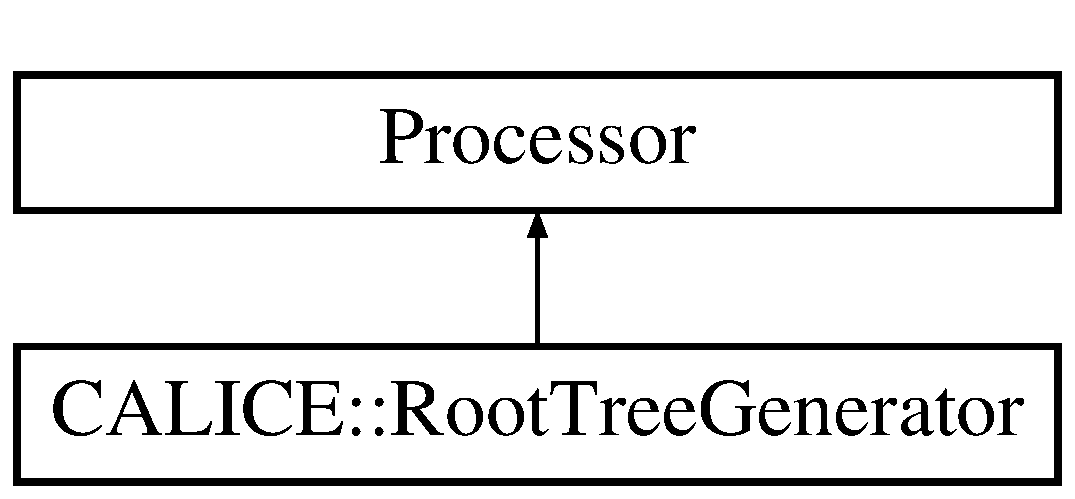
\includegraphics[height=2.000000cm]{classCALICE_1_1RootTreeGenerator}
\end{center}
\end{figure}
\subsection*{Public Member Functions}
\begin{DoxyCompactItemize}
\item 
virtual Processor $\ast$ {\bfseries new\-Processor} ()\label{classCALICE_1_1RootTreeGenerator_a190c4a59fb38f29b4d21ecf4c27758c3}

\item 
void {\bfseries init} ()\label{classCALICE_1_1RootTreeGenerator_a4e25c5be1410bed1779b7c48db8861ae}

\item 
void {\bfseries process\-Event} (L\-C\-Event $\ast$evt)\label{classCALICE_1_1RootTreeGenerator_a4f7d659ca6c9d90f60a13e698d16d369}

\item 
void {\bfseries end} ()\label{classCALICE_1_1RootTreeGenerator_a4659e1ed27fa7d1ce4863945ab3c32ed}

\end{DoxyCompactItemize}
\subsection*{Protected Attributes}
\begin{DoxyCompactItemize}
\item 
std\-::string {\bfseries \-\_\-input\-Col\-Name}\label{classCALICE_1_1RootTreeGenerator_a45697ed70cf6e099a2020dd714504e97}

\item 
std\-::string {\bfseries \-\_\-prefix}\label{classCALICE_1_1RootTreeGenerator_a40fa892791255b3cf185ae01fc1df8a8}

\item 
T\-File $\ast$ {\bfseries \-\_\-root\-File}\label{classCALICE_1_1RootTreeGenerator_aedbcdb07e45e1b40d7cd8212cba0629f}

\item 
std\-::string {\bfseries \-\_\-root\-File\-Name}\label{classCALICE_1_1RootTreeGenerator_ac0f4cfe564f803f8c1c3ced97d8ce0d1}

\item 
T\-Tree $\ast$ {\bfseries \-\_\-tree\-Labview\-Block}\label{classCALICE_1_1RootTreeGenerator_a9a706fe7be21b16d3a4a8fd1f58ced1f}

\item 
int {\bfseries \-\_\-n\-Hits}\label{classCALICE_1_1RootTreeGenerator_afeb6f7f6fa7f8f90f98556dab8e4843e}

\item 
int {\bfseries \-\_\-\-Bunch\-X\-I\-D}\label{classCALICE_1_1RootTreeGenerator_a263bd06e050d66020d71346b7fe17f94}

\item 
int {\bfseries \-\_\-\-Cycle\-Nr}\label{classCALICE_1_1RootTreeGenerator_a7a11796d640791a6015a9ef546c828cb}

\item 
int {\bfseries \-\_\-\-Chip\-I\-D}\label{classCALICE_1_1RootTreeGenerator_acff8c71e037b9886df76290fd718a2fc}

\item 
int {\bfseries \-\_\-\-A\-S\-I\-C\-Nr}\label{classCALICE_1_1RootTreeGenerator_a2fa8cff4b18af909633f82a4abb417f3}

\item 
int {\bfseries \-\_\-\-Evt\-Nr}\label{classCALICE_1_1RootTreeGenerator_a5ecdacceba84880bda93af94d9ed8e64}

\item 
int {\bfseries \-\_\-\-Channel}\label{classCALICE_1_1RootTreeGenerator_ac5c4be539f3cca086c6e84861b7dc1fc}

\item 
int {\bfseries \-\_\-\-T\-D\-C}\label{classCALICE_1_1RootTreeGenerator_afe617610463d32361b66694ee8b0eb81}

\item 
int {\bfseries \-\_\-\-A\-D\-C}\label{classCALICE_1_1RootTreeGenerator_a17be8de3b6d4141fc160b9786d8a490a}

\item 
int {\bfseries \-\_\-x\-Pos}\label{classCALICE_1_1RootTreeGenerator_a5cb40db584a71f4fee52632af926d557}

\item 
int {\bfseries \-\_\-y\-Pos}\label{classCALICE_1_1RootTreeGenerator_a3b7c14462377dbf7f2aa7b567df36f07}

\item 
int {\bfseries \-\_\-\-Hit\-Bit}\label{classCALICE_1_1RootTreeGenerator_afb3bc01afed020817d8a85d4f44cdb9a}

\item 
int {\bfseries \-\_\-\-Gain\-Bit}\label{classCALICE_1_1RootTreeGenerator_ae14d571f1c455371bc5bc3ae391b9f22}

\end{DoxyCompactItemize}
\subsection*{Static Private Attributes}
\begin{DoxyCompactItemize}
\item 
static std\-::map$<$ T\-Tree \\*
$\ast$, {\bf Root\-Tree\-Generator} $\ast$ $>$ {\bfseries \-\_\-tree\-Filler\-Map}\label{classCALICE_1_1RootTreeGenerator_a1edff2386c6a6051202d21be447fea69}

\item 
static std\-::map$<$ T\-Tree \\*
$\ast$, {\bf Root\-Tree\-Generator} $\ast$ $>$ {\bfseries \-\_\-tree\-Owner\-Map}\label{classCALICE_1_1RootTreeGenerator_a331544fd3dfee404ad0d1c5492741ad4}

\item 
static std\-::map$<$ T\-File \\*
$\ast$, {\bf Root\-Tree\-Generator} $\ast$ $>$ {\bfseries \-\_\-file\-Owner\-Map}\label{classCALICE_1_1RootTreeGenerator_aaabe9bfde58f05c43dfa886545fa68ee}

\end{DoxyCompactItemize}


\subsection{Detailed Description}
Class to process Labview raw. 

\begin{DoxyAuthor}{Author}
\-: Shaojun Lu D\-E\-S\-Y 
\end{DoxyAuthor}
\begin{DoxyDate}{Date}
Nov 15 2012 
\end{DoxyDate}


Definition at line 24 of file Root\-Tree\-Generator.\-hh.



The documentation for this class was generated from the following files\-:\begin{DoxyCompactItemize}
\item 
Root\-Tree\-Generator.\-hh\item 
Root\-Tree\-Generator.\-cc\end{DoxyCompactItemize}

\section{C\-A\-L\-I\-C\-E\-:\-:Root\-Tree\-Generator2 Class Reference}
\label{classCALICE_1_1RootTreeGenerator2}\index{C\-A\-L\-I\-C\-E\-::\-Root\-Tree\-Generator2@{C\-A\-L\-I\-C\-E\-::\-Root\-Tree\-Generator2}}


Class to process Labview raw.  




{\ttfamily \#include $<$Root\-Tree\-Generator2.\-hh$>$}

Inheritance diagram for C\-A\-L\-I\-C\-E\-:\-:Root\-Tree\-Generator2\-:\begin{figure}[H]
\begin{center}
\leavevmode
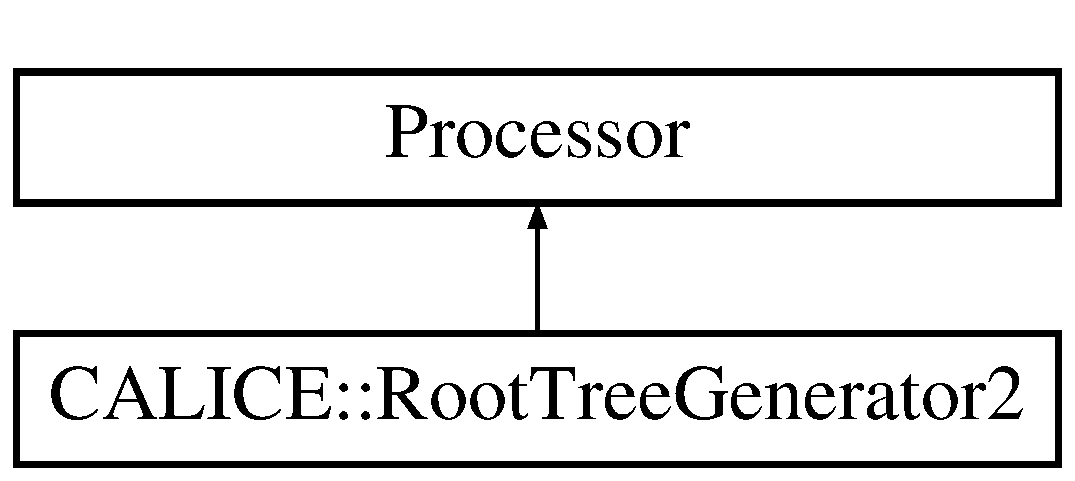
\includegraphics[height=2.000000cm]{classCALICE_1_1RootTreeGenerator2}
\end{center}
\end{figure}
\subsection*{Public Member Functions}
\begin{DoxyCompactItemize}
\item 
virtual Processor $\ast$ {\bfseries new\-Processor} ()\label{classCALICE_1_1RootTreeGenerator2_ab4853d325591a5a66bcb9ebc16cbb136}

\item 
void {\bfseries init} ()\label{classCALICE_1_1RootTreeGenerator2_a80c7d615ad996292e02080c89a7da898}

\item 
void {\bfseries process\-Event} (L\-C\-Event $\ast$evt)\label{classCALICE_1_1RootTreeGenerator2_aca785fa947fe4759fddb0d3dfc417aaa}

\item 
void {\bfseries end} ()\label{classCALICE_1_1RootTreeGenerator2_ad8313adc1a956f6c5b5d24c6174e8c7c}

\end{DoxyCompactItemize}
\subsection*{Protected Attributes}
\begin{DoxyCompactItemize}
\item 
std\-::string {\bfseries \-\_\-input\-Col\-Name}\label{classCALICE_1_1RootTreeGenerator2_a6d97d1cb478d4b9f9ad07d9f931d85c3}

\item 
T\-File $\ast$ {\bfseries \-\_\-root\-File}\label{classCALICE_1_1RootTreeGenerator2_a08632a2ad60e68621fcb6057e30a4eac}

\item 
std\-::string {\bfseries \-\_\-root\-File\-Name}\label{classCALICE_1_1RootTreeGenerator2_ab7abbc742f5582e197cef4f90d7eb36b}

\item 
T\-Tree $\ast$ {\bfseries \-\_\-tree}\label{classCALICE_1_1RootTreeGenerator2_aa67a509d3dab33a262220f7a75142b24}

\item 
double {\bfseries \-\_\-\-Esum\-\_\-\-Layer} [500]\label{classCALICE_1_1RootTreeGenerator2_aedb545467debf9bbe2d804c563cc801c}

\item 
double {\bfseries \-\_\-\-Esum}\label{classCALICE_1_1RootTreeGenerator2_a1ca6108c11d35a075c8e4b5c73ec47a6}

\item 
int {\bfseries \-\_\-event\-\_\-num}\label{classCALICE_1_1RootTreeGenerator2_a4e67941217c6c2c47667ab4e8704205e}

\item 
int {\bfseries n\-Hits}\label{classCALICE_1_1RootTreeGenerator2_afa5acbbee145772c75b2827d22a65215}

\item 
int {\bfseries \-\_\-n\-Hits\-\_\-\-Layer} [500]\label{classCALICE_1_1RootTreeGenerator2_aba262ed115b31d6232e74d4e0cf1ab11}

\item 
int {\bfseries K} [M\-A\-X\-C\-E\-L\-L\-S]\label{classCALICE_1_1RootTreeGenerator2_a342a74fb9c58d7979f235fdfa397810b}

\item 
int {\bfseries I} [M\-A\-X\-C\-E\-L\-L\-S]\label{classCALICE_1_1RootTreeGenerator2_adf394c456c8c971690e5527cbb28b489}

\item 
int {\bfseries J} [M\-A\-X\-C\-E\-L\-L\-S]\label{classCALICE_1_1RootTreeGenerator2_a8ae43ce288d7ca3c0ba9ec24ce1c7423}

\item 
float {\bfseries hit\-Energy} [M\-A\-X\-C\-E\-L\-L\-S]\label{classCALICE_1_1RootTreeGenerator2_af193968dbbbced70a48cb8c91542b63b}

\item 
float {\bfseries hit\-Pos} [M\-A\-X\-C\-E\-L\-L\-S][3]\label{classCALICE_1_1RootTreeGenerator2_a4643eefe73766b7c5f7a07fcd774dd3e}

\item 
float {\bfseries hit\-Timestamp} [M\-A\-X\-C\-E\-L\-L\-S]\label{classCALICE_1_1RootTreeGenerator2_a3b0120528cb9709ead78bf63759d843c}

\end{DoxyCompactItemize}


\subsection{Detailed Description}
Class to process Labview raw. 

\begin{DoxyAuthor}{Author}
\-: Shaojun Lu D\-E\-S\-Y 
\end{DoxyAuthor}
\begin{DoxyDate}{Date}
Nov 15 2012 
\end{DoxyDate}


Definition at line 25 of file Root\-Tree\-Generator2.\-hh.



The documentation for this class was generated from the following files\-:\begin{DoxyCompactItemize}
\item 
Root\-Tree\-Generator2.\-hh\item 
Root\-Tree\-Generator2.\-cc\end{DoxyCompactItemize}

\section{C\-A\-L\-I\-C\-E\-:\-:Root\-Tree\-Generator3 Class Reference}
\label{classCALICE_1_1RootTreeGenerator3}\index{C\-A\-L\-I\-C\-E\-::\-Root\-Tree\-Generator3@{C\-A\-L\-I\-C\-E\-::\-Root\-Tree\-Generator3}}


Class to process Labview raw.  




{\ttfamily \#include $<$Root\-Tree\-Generator3.\-hh$>$}

Inheritance diagram for C\-A\-L\-I\-C\-E\-:\-:Root\-Tree\-Generator3\-:\begin{figure}[H]
\begin{center}
\leavevmode
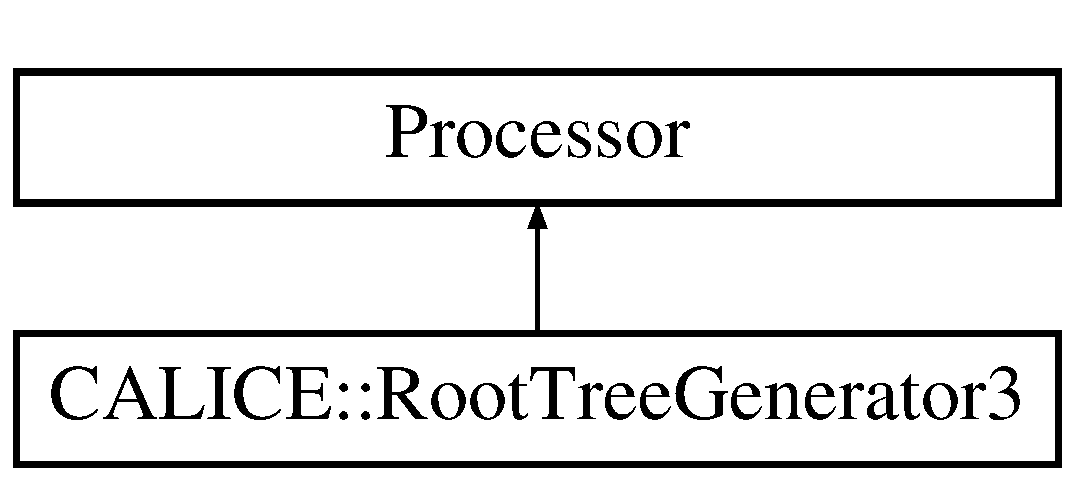
\includegraphics[height=2.000000cm]{classCALICE_1_1RootTreeGenerator3}
\end{center}
\end{figure}
\subsection*{Public Member Functions}
\begin{DoxyCompactItemize}
\item 
virtual Processor $\ast$ {\bfseries new\-Processor} ()\label{classCALICE_1_1RootTreeGenerator3_a1385eeb9f0fa76ace54e2176f995c831}

\item 
void {\bfseries init} ()\label{classCALICE_1_1RootTreeGenerator3_a994dbd1c8750e4d88b8ebdedf90f34aa}

\item 
void {\bfseries process\-Event} (L\-C\-Event $\ast$evt)\label{classCALICE_1_1RootTreeGenerator3_a4f2ca19228fdd754e01b616665254f86}

\item 
void {\bfseries end} ()\label{classCALICE_1_1RootTreeGenerator3_a12de0fe12752ee8db6d40ea63dfa91b6}

\item 
void {\bfseries register\-Branches} (T\-Tree $\ast$host\-Tree)\label{classCALICE_1_1RootTreeGenerator3_a14c95a9a596c0fa8bbbf171f26f67238}

\item 
void {\bfseries Fill\-Variable} (L\-C\-Event $\ast$evt)\label{classCALICE_1_1RootTreeGenerator3_a07bde3d14b4a5bc90f24978a3e8b95d5}

\end{DoxyCompactItemize}
\subsection*{Protected Attributes}
\begin{DoxyCompactItemize}
\item 
std\-::string {\bfseries \-\_\-input\-Col\-Name}\label{classCALICE_1_1RootTreeGenerator3_a34632b4305502a19071bc7ce5bb4bb9d}

\item 
std\-::string {\bfseries \-\_\-prefix}\label{classCALICE_1_1RootTreeGenerator3_a28a8501057a0cc2586b42f50ea341c71}

\item 
T\-File $\ast$ {\bfseries \-\_\-root\-File}\label{classCALICE_1_1RootTreeGenerator3_aa4ec8b9bbe64b45b8d88b07164c8df0b}

\item 
std\-::string {\bfseries \-\_\-root\-File\-Name}\label{classCALICE_1_1RootTreeGenerator3_a49845156d4774dbeadb167fc1583de47}

\item 
T\-Tree $\ast$ {\bfseries \-\_\-tree\-Labview\-Block}\label{classCALICE_1_1RootTreeGenerator3_a57ab8527e5a4a179f7894d4a4acbafb3}

\item 
\begin{tabbing}
xx\=xx\=xx\=xx\=xx\=xx\=xx\=xx\=xx\=\kill
struct \{\\
\>int {\bfseries iEvt}\\
\>int {\bfseries nHits}\\
\>int {\bfseries BunchXID} [MAXCELLS]\\
\>int {\bfseries CycleNr} [MAXCELLS]\\
\>int {\bfseries ChipID} [MAXCELLS]\\
\>int {\bfseries EvtNr} [MAXCELLS]\\
\>int {\bfseries Channel} [MAXCELLS]\\
\>int {\bfseries TDC} [MAXCELLS]\\
\>int {\bfseries ADC} [MAXCELLS]\\
\>int {\bfseries HitBit} [MAXCELLS]\\
\>int {\bfseries GainBit} [MAXCELLS]\\
\} {\bfseries \_hFill}\label{classCALICE_1_1RootTreeGenerator3_af5b939071eb0a559e58e5956f47b5c8a}
\\

\end{tabbing}\end{DoxyCompactItemize}
\subsection*{Static Protected Attributes}
\begin{DoxyCompactItemize}
\item 
static const unsigned int {\bfseries M\-A\-X\-C\-E\-L\-L\-S} = 7609\label{classCALICE_1_1RootTreeGenerator3_ab5afb056b4e112ca55da25fbcd13bddf}

\end{DoxyCompactItemize}
\subsection*{Private Attributes}
\begin{DoxyCompactItemize}
\item 
int {\bfseries ievt}\label{classCALICE_1_1RootTreeGenerator3_a38ebd481e4c45711638c39045182a090}

\item 
int {\bfseries run\-Number}\label{classCALICE_1_1RootTreeGenerator3_ac3a63c5110451b2f7c25f2870394b366}

\item 
int {\bfseries event\-Number}\label{classCALICE_1_1RootTreeGenerator3_a5ee1694157b036ac1b9b0b2fa6dd4f31}

\item 
int {\bfseries Timestamp}\label{classCALICE_1_1RootTreeGenerator3_afcacb608a22273864c315acbbd47e680}

\end{DoxyCompactItemize}
\subsection*{Static Private Attributes}
\begin{DoxyCompactItemize}
\item 
static std\-::map$<$ T\-Tree \\*
$\ast$, {\bf Root\-Tree\-Generator3} $\ast$ $>$ {\bfseries \-\_\-tree\-Filler\-Map}\label{classCALICE_1_1RootTreeGenerator3_aaff1fa336e4bdad0b8c53b2eabae7a7a}

\item 
static std\-::map$<$ T\-Tree \\*
$\ast$, {\bf Root\-Tree\-Generator3} $\ast$ $>$ {\bfseries \-\_\-tree\-Owner\-Map}\label{classCALICE_1_1RootTreeGenerator3_ac03ad28c9c5c1aabf480cc116f2b1a08}

\item 
static std\-::map$<$ T\-File \\*
$\ast$, {\bf Root\-Tree\-Generator3} $\ast$ $>$ {\bfseries \-\_\-file\-Owner\-Map}\label{classCALICE_1_1RootTreeGenerator3_a3ae960ab337dc179d5e62407b172ace7}

\item 
static const double {\bfseries I\-N\-V\-A\-L\-I\-D} = -\/F\-L\-T\-\_\-\-M\-A\-X\label{classCALICE_1_1RootTreeGenerator3_a08a34f6003acb82140e27427937ed6d1}

\end{DoxyCompactItemize}


\subsection{Detailed Description}
Class to process Labview raw. 

\begin{DoxyAuthor}{Author}
\-: Shaojun Lu D\-E\-S\-Y 
\end{DoxyAuthor}
\begin{DoxyDate}{Date}
Nov 15 2012 
\end{DoxyDate}


Definition at line 21 of file Root\-Tree\-Generator3.\-hh.



The documentation for this class was generated from the following files\-:\begin{DoxyCompactItemize}
\item 
Root\-Tree\-Generator3.\-hh\item 
Root\-Tree\-Generator3.\-cc\end{DoxyCompactItemize}

\section{C\-A\-L\-I\-C\-E\-:\-:Root\-Tree\-Generator\-E\-U\-D\-A\-Q2016 Class Reference}
\label{classCALICE_1_1RootTreeGeneratorEUDAQ2016}\index{C\-A\-L\-I\-C\-E\-::\-Root\-Tree\-Generator\-E\-U\-D\-A\-Q2016@{C\-A\-L\-I\-C\-E\-::\-Root\-Tree\-Generator\-E\-U\-D\-A\-Q2016}}


Class to process Labview raw.  




{\ttfamily \#include $<$Root\-Tree\-Generator\-E\-U\-D\-A\-Q2016.\-hh$>$}

Inheritance diagram for C\-A\-L\-I\-C\-E\-:\-:Root\-Tree\-Generator\-E\-U\-D\-A\-Q2016\-:\begin{figure}[H]
\begin{center}
\leavevmode
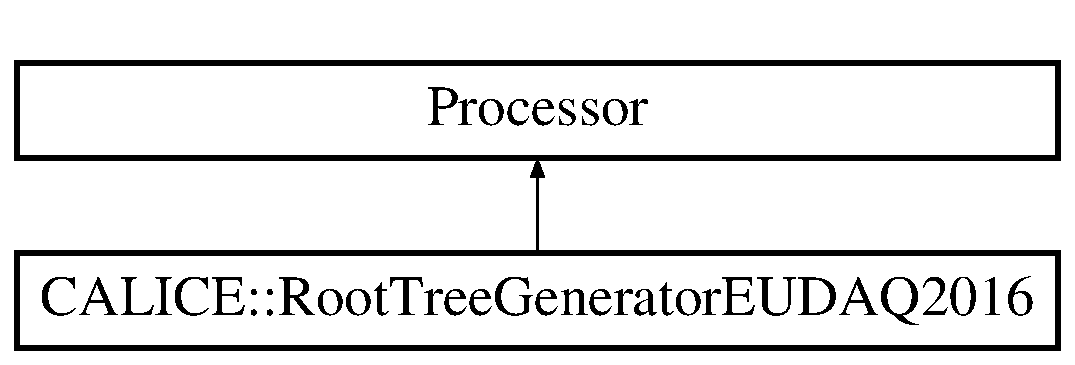
\includegraphics[height=2.000000cm]{classCALICE_1_1RootTreeGeneratorEUDAQ2016}
\end{center}
\end{figure}
\subsection*{Public Member Functions}
\begin{DoxyCompactItemize}
\item 
virtual Processor $\ast$ {\bfseries new\-Processor} ()\label{classCALICE_1_1RootTreeGeneratorEUDAQ2016_adb6517ac6d1e813d05d19d0a118caa8c}

\item 
void {\bfseries init} ()\label{classCALICE_1_1RootTreeGeneratorEUDAQ2016_a2eb9c18fbb3422bd9a6800565f4c9d07}

\item 
void {\bfseries process\-Event} (L\-C\-Event $\ast$evt)\label{classCALICE_1_1RootTreeGeneratorEUDAQ2016_a5d169a6cdf7f3471a2a150dd4723f377}

\item 
void {\bfseries end} ()\label{classCALICE_1_1RootTreeGeneratorEUDAQ2016_acc5e873edc240b1789ba394087e2c26e}

\item 
void {\bfseries register\-Branches} (T\-Tree $\ast$host\-Tree)\label{classCALICE_1_1RootTreeGeneratorEUDAQ2016_a56d658a01150d2c00b4a5c37807f17bf}

\item 
void {\bfseries Fill\-Variable} (L\-C\-Collection $\ast$col)\label{classCALICE_1_1RootTreeGeneratorEUDAQ2016_ae758d4492e1ec6e7dc180476294e0754}

\end{DoxyCompactItemize}
\subsection*{Protected Attributes}
\begin{DoxyCompactItemize}
\item 
std\-::string {\bfseries \-\_\-input\-Col\-Name}\label{classCALICE_1_1RootTreeGeneratorEUDAQ2016_ac2e510fb22f7812c6daee89b12ac9c3b}

\item 
std\-::string {\bfseries \-\_\-prefix}\label{classCALICE_1_1RootTreeGeneratorEUDAQ2016_a322f00e45091686e6d9b9c8ead72dd4a}

\item 
T\-File $\ast$ {\bfseries \-\_\-root\-File}\label{classCALICE_1_1RootTreeGeneratorEUDAQ2016_a909e0073fa5d088d1c244d36268a31f0}

\item 
std\-::string {\bfseries \-\_\-root\-File\-Name}\label{classCALICE_1_1RootTreeGeneratorEUDAQ2016_a8bfc2d4f1ab531348913b77c6ac1ee12}

\item 
T\-Tree $\ast$ {\bfseries \-\_\-tree\-E\-U\-D\-A\-Q\-Block2016}\label{classCALICE_1_1RootTreeGeneratorEUDAQ2016_afa4dbf097c8ef24ba83e4a485d416d94}

\item 
int {\bfseries i\-Evt}\label{classCALICE_1_1RootTreeGeneratorEUDAQ2016_a07fada508d390fda146f131c66046efc}

\item 
int {\bfseries n\-Hits}\label{classCALICE_1_1RootTreeGeneratorEUDAQ2016_a29287f1fa8ec15486bd535499510fa26}

\item 
int {\bfseries V\-Calib}\label{classCALICE_1_1RootTreeGeneratorEUDAQ2016_ab37854f9741555e42f9b6a2dc4caad1e}

\item 
std\-::vector$<$ int $>$ $\ast$ {\bfseries Bunch\-X\-I\-D}\label{classCALICE_1_1RootTreeGeneratorEUDAQ2016_a07c009bbb352b95a0fa618e7fe39aaa5}

\item 
std\-::vector$<$ int $>$ $\ast$ {\bfseries Cycle\-Nr}\label{classCALICE_1_1RootTreeGeneratorEUDAQ2016_a5d00694a07f125233a8c4309d761a8f6}

\item 
std\-::vector$<$ int $>$ $\ast$ {\bfseries Chip\-I\-D}\label{classCALICE_1_1RootTreeGeneratorEUDAQ2016_a5462d4c744d42665604d3b2d5a1fedaf}

\item 
std\-::vector$<$ int $>$ $\ast$ {\bfseries Evt\-Nr}\label{classCALICE_1_1RootTreeGeneratorEUDAQ2016_abadc209886e81c7bfa3aa2b73b815bf0}

\item 
std\-::vector$<$ int $>$ $\ast$ {\bfseries Channel}\label{classCALICE_1_1RootTreeGeneratorEUDAQ2016_af1824afeb2b1ffa825bb3ddd14722ef7}

\item 
std\-::vector$<$ int $>$ $\ast$ {\bfseries T\-D\-C}\label{classCALICE_1_1RootTreeGeneratorEUDAQ2016_a170d726c9f6d8398973511c3b6e81319}

\item 
std\-::vector$<$ int $>$ $\ast$ {\bfseries A\-D\-C}\label{classCALICE_1_1RootTreeGeneratorEUDAQ2016_af43d4395913a19fa1ef34e276bf99f41}

\item 
std\-::vector$<$ int $>$ $\ast$ {\bfseries Hit\-Bit}\label{classCALICE_1_1RootTreeGeneratorEUDAQ2016_a01b238a4a713eb52c946feac98056bcf}

\item 
std\-::vector$<$ int $>$ $\ast$ {\bfseries Gain\-Bit}\label{classCALICE_1_1RootTreeGeneratorEUDAQ2016_a32a8146a291432eb23487db37c41a110}

\end{DoxyCompactItemize}
\subsection*{Private Attributes}
\begin{DoxyCompactItemize}
\item 
int {\bfseries \-\_\-n\-Hits}\label{classCALICE_1_1RootTreeGeneratorEUDAQ2016_a735601e0c7ba867dd33220b67fdac246}

\item 
int {\bfseries ievt}\label{classCALICE_1_1RootTreeGeneratorEUDAQ2016_a7a5b38d420f5c9bbffebed4a12fbc686}

\item 
int {\bfseries run\-Number}\label{classCALICE_1_1RootTreeGeneratorEUDAQ2016_a9fa143e155360b6f645d0b19f5e83efa}

\item 
int {\bfseries event\-Number}\label{classCALICE_1_1RootTreeGeneratorEUDAQ2016_a87e4a3f01d9619d80dee5e3ce99e4bd3}

\item 
int {\bfseries Timestamp}\label{classCALICE_1_1RootTreeGeneratorEUDAQ2016_a9559dfea2413851744d5aa51f0634b25}

\end{DoxyCompactItemize}
\subsection*{Static Private Attributes}
\begin{DoxyCompactItemize}
\item 
static std\-::map$<$ T\-Tree \\*
$\ast$, {\bf Root\-Tree\-Generator\-E\-U\-D\-A\-Q2016} $\ast$ $>$ {\bfseries \-\_\-tree\-Filler\-Map}\label{classCALICE_1_1RootTreeGeneratorEUDAQ2016_a903416643c6674afccaea80284251609}

\item 
static std\-::map$<$ T\-Tree \\*
$\ast$, {\bf Root\-Tree\-Generator\-E\-U\-D\-A\-Q2016} $\ast$ $>$ {\bfseries \-\_\-tree\-Owner\-Map}\label{classCALICE_1_1RootTreeGeneratorEUDAQ2016_a3308044bfa6b2926022e7b2d5c332535}

\item 
static std\-::map$<$ T\-File \\*
$\ast$, {\bf Root\-Tree\-Generator\-E\-U\-D\-A\-Q2016} $\ast$ $>$ {\bfseries \-\_\-file\-Owner\-Map}\label{classCALICE_1_1RootTreeGeneratorEUDAQ2016_a15406fbbea39ab6fbca1f5feacfd2bfd}

\item 
static const double {\bfseries I\-N\-V\-A\-L\-I\-D} = -\/F\-L\-T\-\_\-\-M\-A\-X\label{classCALICE_1_1RootTreeGeneratorEUDAQ2016_ab2522fe7595699b48a20555da4923c39}

\end{DoxyCompactItemize}


\subsection{Detailed Description}
Class to process Labview raw. 

\begin{DoxyAuthor}{Author}
\-: Shaojun Lu D\-E\-S\-Y 
\end{DoxyAuthor}
\begin{DoxyDate}{Date}
Nov 15 2012 
\end{DoxyDate}


Definition at line 22 of file Root\-Tree\-Generator\-E\-U\-D\-A\-Q2016.\-hh.



The documentation for this class was generated from the following files\-:\begin{DoxyCompactItemize}
\item 
Root\-Tree\-Generator\-E\-U\-D\-A\-Q2016.\-hh\item 
Root\-Tree\-Generator\-E\-U\-D\-A\-Q2016.\-cc\end{DoxyCompactItemize}

\section{marlin\-:\-:Root\-Write\-Engine Class Reference}
\label{classmarlin_1_1RootWriteEngine}\index{marlin\-::\-Root\-Write\-Engine@{marlin\-::\-Root\-Write\-Engine}}


Abstract base class of callback classes for the Root\-Tree\-Write processor Abstract interface for a Root\-Tree\-Writer-\/engine.  




{\ttfamily \#include $<$Root\-Write\-Engine.\-hh$>$}

\subsection*{Public Member Functions}
\begin{DoxyCompactItemize}
\item 
{\bf Root\-Write\-Engine} (Root\-Tree\-Writer $\ast$host)
\begin{DoxyCompactList}\small\item\em constructor \end{DoxyCompactList}\item 
virtual const std\-::string \& {\bf get\-Engine\-Name} ()=0
\begin{DoxyCompactList}\small\item\em Returns the name of the engine to the Root\-Tree\-Writer processor. \end{DoxyCompactList}\item 
virtual void {\bf register\-Parameters} ()=0
\begin{DoxyCompactList}\small\item\em Used to register steering parameters. \end{DoxyCompactList}\item 
virtual void {\bf register\-Branches} (T\-Tree $\ast$t)=0
\begin{DoxyCompactList}\small\item\em Implement to register local variables to the output tree. \end{DoxyCompactList}\item 
virtual void {\bf fill\-Variables} (E\-V\-E\-N\-T\-::\-L\-C\-Event $\ast$evt)=0
\begin{DoxyCompactList}\small\item\em Implement this to extract the variables which you want to fill into the {\itshape R\-O\-O\-T} tree from the event. \end{DoxyCompactList}\end{DoxyCompactItemize}
\subsection*{Protected Attributes}
\begin{DoxyCompactItemize}
\item 
Root\-Tree\-Writer \& {\bfseries \-\_\-host\-Processor}\label{classmarlin_1_1RootWriteEngine_ab53e690ff0f758b27f4ef45b87f3d3ce}

\end{DoxyCompactItemize}


\subsection{Detailed Description}
Abstract base class of callback classes for the Root\-Tree\-Write processor Abstract interface for a Root\-Tree\-Writer-\/engine. 

Implement an descendant of this class to add variables to the output tree of the Root\-Tree\-Writer\-Processor. After that add the new {\itshape engine} to the list of writer engines in the Root\-Tree\-Writer processor 

Definition at line 29 of file Root\-Write\-Engine.\-hh.



\subsection{Constructor \& Destructor Documentation}
\index{marlin\-::\-Root\-Write\-Engine@{marlin\-::\-Root\-Write\-Engine}!Root\-Write\-Engine@{Root\-Write\-Engine}}
\index{Root\-Write\-Engine@{Root\-Write\-Engine}!marlin::RootWriteEngine@{marlin\-::\-Root\-Write\-Engine}}
\subsubsection[{Root\-Write\-Engine}]{\setlength{\rightskip}{0pt plus 5cm}marlin\-::\-Root\-Write\-Engine\-::\-Root\-Write\-Engine (
\begin{DoxyParamCaption}
\item[{Root\-Tree\-Writer $\ast$}]{host}
\end{DoxyParamCaption}
)\hspace{0.3cm}{\ttfamily [inline]}}\label{classmarlin_1_1RootWriteEngine_a9a2f783fbd71d43487cb94feee09210a}


constructor 

\begin{DoxyVerb}\param[in] host pointer to the RootTreeWriter processor the constructor
of a derived class must pass this pointer to this base class e.g.@verbatim 
\end{DoxyVerb}
 /// Somee\-Write\-Engine( Root\-Tree\-Writer$\ast$ host )\-:Root\-Write\-Engine(host), /// \-\_\-engine\-Name(\char`\"{}\-Some\-Write\-Engine\char`\"{}) /// \{\}  

Definition at line 38 of file Root\-Write\-Engine.\-hh.



\subsection{Member Function Documentation}
\index{marlin\-::\-Root\-Write\-Engine@{marlin\-::\-Root\-Write\-Engine}!fill\-Variables@{fill\-Variables}}
\index{fill\-Variables@{fill\-Variables}!marlin::RootWriteEngine@{marlin\-::\-Root\-Write\-Engine}}
\subsubsection[{fill\-Variables}]{\setlength{\rightskip}{0pt plus 5cm}virtual void marlin\-::\-Root\-Write\-Engine\-::fill\-Variables (
\begin{DoxyParamCaption}
\item[{E\-V\-E\-N\-T\-::\-L\-C\-Event $\ast$}]{evt}
\end{DoxyParamCaption}
)\hspace{0.3cm}{\ttfamily [pure virtual]}}\label{classmarlin_1_1RootWriteEngine_ace823bd839cee7e8c8755e60c4cc7134}


Implement this to extract the variables which you want to fill into the {\itshape R\-O\-O\-T} tree from the event. 

Write the value of the variables you want to add to the tree to the member variables, which you registered to the {\itshape R\-O\-O\-T} tree. The Root\-Tree\-Writer will call T\-Tree\-::\-Fill() for you. 
\begin{DoxyParams}{Parameters}
{\em evt} & the current event \\
\hline
\end{DoxyParams}
\index{marlin\-::\-Root\-Write\-Engine@{marlin\-::\-Root\-Write\-Engine}!get\-Engine\-Name@{get\-Engine\-Name}}
\index{get\-Engine\-Name@{get\-Engine\-Name}!marlin::RootWriteEngine@{marlin\-::\-Root\-Write\-Engine}}
\subsubsection[{get\-Engine\-Name}]{\setlength{\rightskip}{0pt plus 5cm}virtual const std\-::string\& marlin\-::\-Root\-Write\-Engine\-::get\-Engine\-Name (
\begin{DoxyParamCaption}
{}
\end{DoxyParamCaption}
)\hspace{0.3cm}{\ttfamily [pure virtual]}}\label{classmarlin_1_1RootWriteEngine_a31e38120fe60efcb15666fd569ba5862}


Returns the name of the engine to the Root\-Tree\-Writer processor. 

\begin{DoxyReturn}{Returns}
Must return a string with the engine name. 
\end{DoxyReturn}
\begin{DoxyRefDesc}{Todo}
\item[{\bf Todo}]fixme\-: should be const, but must be declared const in implementations too. Need to fix all existing engines?!? \end{DoxyRefDesc}
\index{marlin\-::\-Root\-Write\-Engine@{marlin\-::\-Root\-Write\-Engine}!register\-Branches@{register\-Branches}}
\index{register\-Branches@{register\-Branches}!marlin::RootWriteEngine@{marlin\-::\-Root\-Write\-Engine}}
\subsubsection[{register\-Branches}]{\setlength{\rightskip}{0pt plus 5cm}virtual void marlin\-::\-Root\-Write\-Engine\-::register\-Branches (
\begin{DoxyParamCaption}
\item[{T\-Tree $\ast$}]{t}
\end{DoxyParamCaption}
)\hspace{0.3cm}{\ttfamily [pure virtual]}}\label{classmarlin_1_1RootWriteEngine_a95baa0248152dc5807ba6bc9396b334e}


Implement to register local variables to the output tree. 

\begin{DoxyVerb}\param[in] t pointer to the \a ROOT tree, which the RootTreeWriter processor fills at the
end of each event.
Usually the implementation looks like@verbatim 
\end{DoxyVerb}
 /// host\-Tree-\/$>$Branch(\char`\"{}variable\char`\"{},\&\-\_\-variable\char`\"{} ,\char`\"{}variable/\-F" ); /// . But you can add any type of branch you like. \index{marlin\-::\-Root\-Write\-Engine@{marlin\-::\-Root\-Write\-Engine}!register\-Parameters@{register\-Parameters}}
\index{register\-Parameters@{register\-Parameters}!marlin::RootWriteEngine@{marlin\-::\-Root\-Write\-Engine}}
\subsubsection[{register\-Parameters}]{\setlength{\rightskip}{0pt plus 5cm}virtual void marlin\-::\-Root\-Write\-Engine\-::register\-Parameters (
\begin{DoxyParamCaption}
{}
\end{DoxyParamCaption}
)\hspace{0.3cm}{\ttfamily [pure virtual]}}\label{classmarlin_1_1RootWriteEngine_ae12b70923768043fa5c1438f078c41d3}


Used to register steering parameters. 

\begin{DoxyVerb}Implement to register \a marlin steering file parameters. Use \a marlin syntax
to register parameters for the calling RootTreeWriter processor.

use@verbatim 
\end{DoxyVerb}
 /// \-\_\-host\-Proc.\-relay\-Register\-Processor\-Parameter(...) /// \-\_\-host\-Proc.\-relay\-Register...() ///  instead of {\itshape marlin} processors\begin{DoxyVerb}register...() \end{DoxyVerb}
 methods 

The documentation for this class was generated from the following file\-:\begin{DoxyCompactItemize}
\item 
Root\-Write\-Engine.\-hh\end{DoxyCompactItemize}

\section{C\-A\-L\-I\-C\-E\-:\-:Split\-Collection\-Processor Class Reference}
\label{classCALICE_1_1SplitCollectionProcessor}\index{C\-A\-L\-I\-C\-E\-::\-Split\-Collection\-Processor@{C\-A\-L\-I\-C\-E\-::\-Split\-Collection\-Processor}}


Processor used to split the E\-U\-D\-A\-Q Collection into 3 Collections for the May/\-June 2018 testbeam.  




{\ttfamily \#include $<$Split\-Collection\-Processor.\-hh$>$}

Inheritance diagram for C\-A\-L\-I\-C\-E\-:\-:Split\-Collection\-Processor\-:\begin{figure}[H]
\begin{center}
\leavevmode
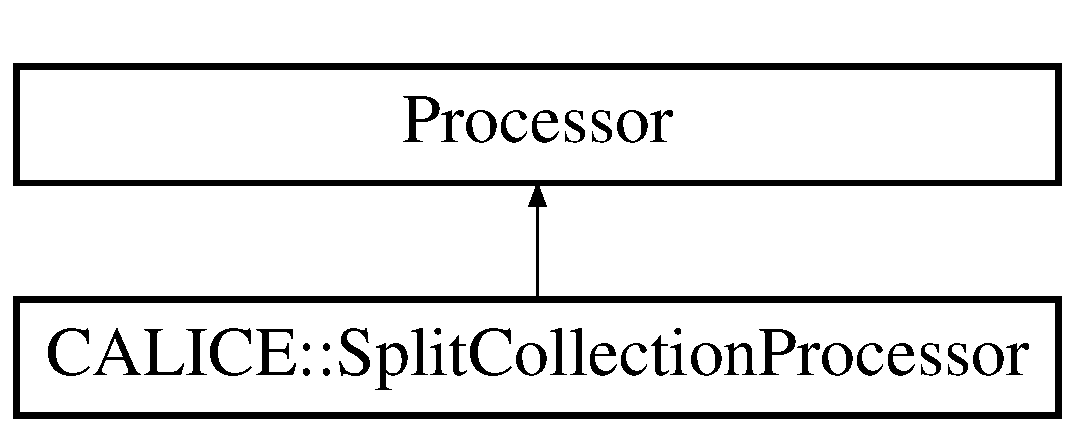
\includegraphics[height=2.000000cm]{classCALICE_1_1SplitCollectionProcessor}
\end{center}
\end{figure}
\subsection*{Public Member Functions}
\begin{DoxyCompactItemize}
\item 
virtual Processor $\ast$ {\bf new\-Processor} ()\label{classCALICE_1_1SplitCollectionProcessor_ab2ffd856a6c36b3f38e271f6244040a1}

\begin{DoxyCompactList}\small\item\em Implementation of new Processor returns pointer to processor. \end{DoxyCompactList}\item 
void {\bf process\-Event} (L\-C\-Event $\ast$evt)\label{classCALICE_1_1SplitCollectionProcessor_ae66e904f58771b3a4c53b8c03e655847}

\begin{DoxyCompactList}\small\item\em Creates events with L\-C\-Genreal\-Object collections from the E\-U\-D\-A\-Q input file and calls all active processors' \doxyref{process\-Event()}{p.}{classCALICE_1_1SplitCollectionProcessor_ae66e904f58771b3a4c53b8c03e655847} and process\-Run\-Header Method. \end{DoxyCompactList}\item 
virtual void {\bf init} ()\label{classCALICE_1_1SplitCollectionProcessor_afdba0a3b5fde6b32bae36bd839b6fec1}

\begin{DoxyCompactList}\small\item\em init method \end{DoxyCompactList}\item 
void {\bfseries Fill\-Container} (L\-C\-Event $\ast$evt)\label{classCALICE_1_1SplitCollectionProcessor_a07834cbe177b763347e11d8765ebdd4f}

\item 
void {\bfseries Fill\-Output\-Collections} (int Chip\-I\-D, {\bf E\-U\-D\-A\-Q\-Block2016} $\ast$l\-Block, L\-C\-Collection\-Vec $\ast$\&col\-Pre\-Shower, L\-C\-Collection\-Vec $\ast$\&col\-H\-C\-A\-L, L\-C\-Collection\-Vec $\ast$\&col\-T\-C)\label{classCALICE_1_1SplitCollectionProcessor_a6955e6e8344094ddfaba11aef96e3f33}

\item 
virtual void {\bf end} ()\label{classCALICE_1_1SplitCollectionProcessor_a03a38ae1b2a40f94167669e2c9d3bd07}

\begin{DoxyCompactList}\small\item\em end method \end{DoxyCompactList}\item 
void {\bf print\-Parameters} ()\label{classCALICE_1_1SplitCollectionProcessor_a10a5ecedc95ff37323e1cbaf6cca1b61}

\begin{DoxyCompactList}\small\item\em print parameters \end{DoxyCompactList}\end{DoxyCompactItemize}
\subsection*{Protected Attributes}
\begin{DoxyCompactItemize}
\item 
std\-::string {\bfseries \-\_\-input\-Col\-Name}\label{classCALICE_1_1SplitCollectionProcessor_ac11c5e0377a6af76a9c9ce66d75eaf8a}

\item 
std\-::string {\bfseries \-\_\-output\-Col\-Name\-Pre\-Shower}\label{classCALICE_1_1SplitCollectionProcessor_a0aa714d717c7c7d31a557a64db14c4b2}

\item 
std\-::string {\bfseries \-\_\-output\-Col\-Name\-H\-C\-A\-L}\label{classCALICE_1_1SplitCollectionProcessor_a0035e1a203d75523e6f3bd39755d3915}

\item 
std\-::string {\bfseries \-\_\-output\-Col\-Name\-T\-C}\label{classCALICE_1_1SplitCollectionProcessor_a5ae3f8b018ac3cb8125ce08ca94574ee}

\item 
std\-::string {\bfseries \-\_\-\-Ahc2\-Hardware\-Connection\-Name}\label{classCALICE_1_1SplitCollectionProcessor_ad15d5840b76e734f4e88c9a95b977194}

\item 
std\-::map$<$ int, int $>$ {\bf \-\_\-\-Hardware\-Connnection\-Container}\label{classCALICE_1_1SplitCollectionProcessor_a6b02fc4ab3802c32846ae30dbab0f814}

\begin{DoxyCompactList}\small\item\em map containing relationship between Chip\-I\-D and Module/\-Chip\-Nb \end{DoxyCompactList}\item 
std\-::string {\bfseries \-\_\-detector\-Type\-Name}\label{classCALICE_1_1SplitCollectionProcessor_afc696ba6c38f9a653c7b567707890a89}

\item 
bool {\bfseries \-\_\-is\-First\-Event}\label{classCALICE_1_1SplitCollectionProcessor_a5bfe4730ea8f6cab2bf51355504d3b28}

\item 
int {\bf \-\_\-run\-Number}\label{classCALICE_1_1SplitCollectionProcessor_af0c27ecd09bfea66903fa7c902f4cee0}

\begin{DoxyCompactList}\small\item\em The run number. \end{DoxyCompactList}\end{DoxyCompactItemize}


\subsection{Detailed Description}
Processor used to split the E\-U\-D\-A\-Q Collection into 3 Collections for the May/\-June 2018 testbeam. 

Definition at line 21 of file Split\-Collection\-Processor.\-hh.



The documentation for this class was generated from the following files\-:\begin{DoxyCompactItemize}
\item 
Split\-Collection\-Processor.\-hh\item 
Split\-Collection\-Processor.\-cc\end{DoxyCompactItemize}

\section{C\-A\-L\-I\-C\-E\-:\-:Temp\-Root\-Tree\-Generator Class Reference}
\label{classCALICE_1_1TempRootTreeGenerator}\index{C\-A\-L\-I\-C\-E\-::\-Temp\-Root\-Tree\-Generator@{C\-A\-L\-I\-C\-E\-::\-Temp\-Root\-Tree\-Generator}}


Class to process Labview raw.  




{\ttfamily \#include $<$Temp\-Root\-Tree\-Generator.\-hh$>$}

Inheritance diagram for C\-A\-L\-I\-C\-E\-:\-:Temp\-Root\-Tree\-Generator\-:\begin{figure}[H]
\begin{center}
\leavevmode
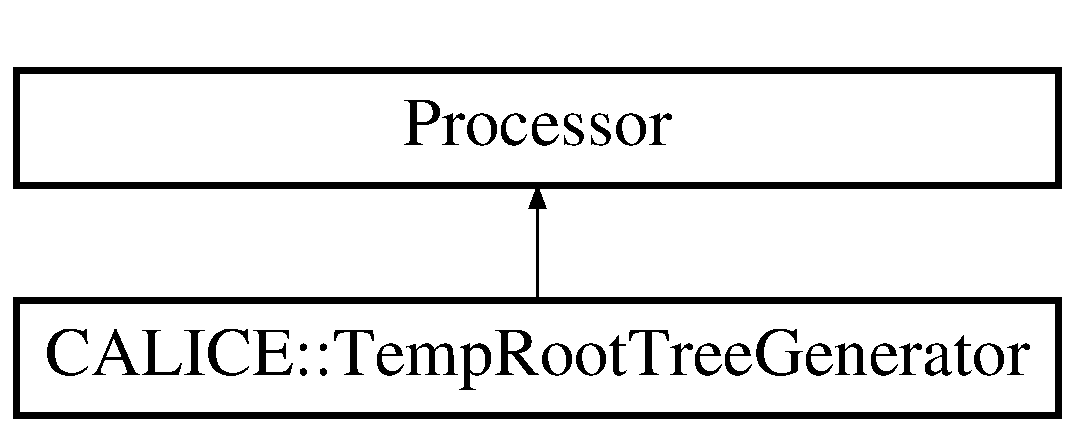
\includegraphics[height=2.000000cm]{classCALICE_1_1TempRootTreeGenerator}
\end{center}
\end{figure}
\subsection*{Public Member Functions}
\begin{DoxyCompactItemize}
\item 
virtual Processor $\ast$ {\bfseries new\-Processor} ()\label{classCALICE_1_1TempRootTreeGenerator_a4683c88fa11fdadc38b174cbd78191df}

\item 
void {\bfseries init} ()\label{classCALICE_1_1TempRootTreeGenerator_a0a85ca935c8d4227cf78ff85745c801f}

\item 
void {\bfseries process\-Event} (L\-C\-Event $\ast$evt)\label{classCALICE_1_1TempRootTreeGenerator_affbf92f531b40ab279bec5764dd798b2}

\item 
void {\bfseries end} ()\label{classCALICE_1_1TempRootTreeGenerator_aebdde734f7d29091114a7c5da186e06f}

\item 
void {\bfseries register\-Branches} (T\-Tree $\ast$host\-Tree)\label{classCALICE_1_1TempRootTreeGenerator_a8c8c4c7c423b1aa404028e59960ba771}

\item 
void {\bfseries Fill\-Variable} (L\-C\-Event $\ast$evt)\label{classCALICE_1_1TempRootTreeGenerator_a3544386c3f78d68615da0c01f437e35e}

\end{DoxyCompactItemize}
\subsection*{Protected Attributes}
\begin{DoxyCompactItemize}
\item 
std\-::string {\bfseries \-\_\-input\-Col\-Name}\label{classCALICE_1_1TempRootTreeGenerator_a08f763e65ab9a64986e987af8ce0117c}

\item 
std\-::string {\bfseries \-\_\-input\-Map\-Name}\label{classCALICE_1_1TempRootTreeGenerator_a5f2a177592ddd414347d76de100dc788}

\item 
std\-::string {\bfseries \-\_\-prefix}\label{classCALICE_1_1TempRootTreeGenerator_a324bde76149073163629a7e9e50c453e}

\item 
T\-File $\ast$ {\bfseries \-\_\-root\-File}\label{classCALICE_1_1TempRootTreeGenerator_add462b67e83bd77baed72038875a81a6}

\item 
std\-::string {\bfseries \-\_\-root\-File\-Name}\label{classCALICE_1_1TempRootTreeGenerator_a0c8aec17e8952dd62d3bfa678ce3eca3}

\item 
T\-Tree $\ast$ {\bfseries \-\_\-tree\-Temp\-Sensor\-Block}\label{classCALICE_1_1TempRootTreeGenerator_a40cc9d843dbba86306d56dbee9218c79}

\item 
\begin{tabbing}
xx\=xx\=xx\=xx\=xx\=xx\=xx\=xx\=xx\=\kill
struct \{\\
\>int {\bfseries nLayers}\\
\>float {\bfseries T1} [MAXPORTS]\\
\>float {\bfseries T2} [MAXPORTS]\\
\>float {\bfseries T3} [MAXPORTS]\\
\>float {\bfseries T4} [MAXPORTS]\\
\>float {\bfseries T5} [MAXPORTS]\\
\>float {\bfseries T6} [MAXPORTS]\\
\>float {\bfseries TDIF} [MAXPORTS]\\
\>float {\bfseries TPWR} [MAXPORTS]\\
\} {\bfseries \_hFill}\label{classCALICE_1_1TempRootTreeGenerator_a48b1a2d44f5fb9c335dbfd88b743ced1}
\\

\end{tabbing}\end{DoxyCompactItemize}
\subsection*{Static Protected Attributes}
\begin{DoxyCompactItemize}
\item 
static const unsigned int {\bfseries M\-A\-X\-P\-O\-R\-T\-S} = 1000\label{classCALICE_1_1TempRootTreeGenerator_ab2162b267c9e1f26729de736c4b2bf8d}

\end{DoxyCompactItemize}
\subsection*{Private Attributes}
\begin{DoxyCompactItemize}
\item 
int {\bfseries run\-Number}\label{classCALICE_1_1TempRootTreeGenerator_ab6b2729ac1b292d2ee2fea66a9594703}

\item 
int {\bfseries event\-Number}\label{classCALICE_1_1TempRootTreeGenerator_a9d25e5c9fd0dbb2f75e1a3e149e45169}

\item 
long64 {\bfseries Timestamp}\label{classCALICE_1_1TempRootTreeGenerator_a987d676226994b2120f47c457551ba09}

\end{DoxyCompactItemize}
\subsection*{Static Private Attributes}
\begin{DoxyCompactItemize}
\item 
static std\-::map$<$ T\-Tree \\*
$\ast$, {\bf Temp\-Root\-Tree\-Generator} $\ast$ $>$ {\bfseries \-\_\-tree\-Filler\-Map}\label{classCALICE_1_1TempRootTreeGenerator_a5aecfdab878099a4ea0a74e4b96652de}

\item 
static std\-::map$<$ T\-Tree \\*
$\ast$, {\bf Temp\-Root\-Tree\-Generator} $\ast$ $>$ {\bfseries \-\_\-tree\-Owner\-Map}\label{classCALICE_1_1TempRootTreeGenerator_a991022195e98911f7e5674c9ad674cce}

\item 
static std\-::map$<$ T\-File \\*
$\ast$, {\bf Temp\-Root\-Tree\-Generator} $\ast$ $>$ {\bfseries \-\_\-file\-Owner\-Map}\label{classCALICE_1_1TempRootTreeGenerator_acf9f072ece6ac7300b4a6ef878bdb947}

\item 
static const double {\bfseries I\-N\-V\-A\-L\-I\-D} = -\/F\-L\-T\-\_\-\-M\-A\-X\label{classCALICE_1_1TempRootTreeGenerator_ab51bc9fd4548675bdad7f48208a3c943}

\end{DoxyCompactItemize}


\subsection{Detailed Description}
Class to process Labview raw. 

\begin{DoxyAuthor}{Author}
\-: Shaojun Lu D\-E\-S\-Y 
\end{DoxyAuthor}
\begin{DoxyDate}{Date}
Nov 15 2012 
\end{DoxyDate}


Definition at line 20 of file Temp\-Root\-Tree\-Generator.\-hh.



The documentation for this class was generated from the following files\-:\begin{DoxyCompactItemize}
\item 
Temp\-Root\-Tree\-Generator.\-hh\item 
Temp\-Root\-Tree\-Generator.\-cc\end{DoxyCompactItemize}

\section{C\-A\-L\-I\-C\-E\-:\-:Temp\-Sensor\-Block Class Reference}
\label{classCALICE_1_1TempSensorBlock}\index{C\-A\-L\-I\-C\-E\-::\-Temp\-Sensor\-Block@{C\-A\-L\-I\-C\-E\-::\-Temp\-Sensor\-Block}}


Class for the Labview Data as acquired by the A\-H\-C\-A\-L Labview.  




{\ttfamily \#include $<$Temp\-Sensor\-Block.\-hh$>$}

Inheritance diagram for C\-A\-L\-I\-C\-E\-:\-:Temp\-Sensor\-Block\-:\begin{figure}[H]
\begin{center}
\leavevmode
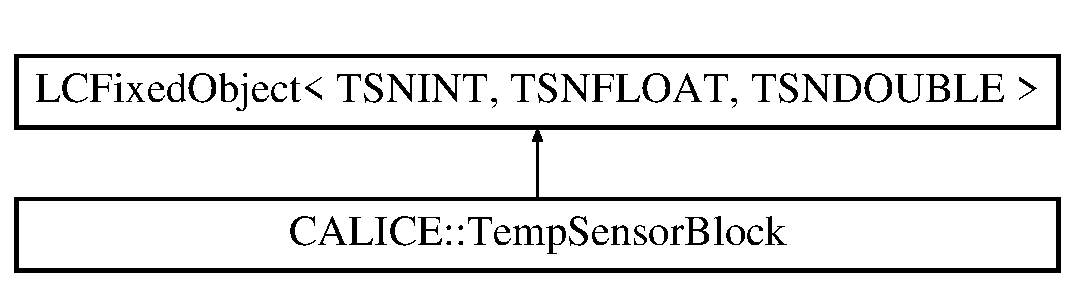
\includegraphics[height=2.000000cm]{classCALICE_1_1TempSensorBlock}
\end{center}
\end{figure}
\subsection*{Public Member Functions}
\begin{DoxyCompactItemize}
\item 
{\bf Temp\-Sensor\-Block} (int Temp\-Sensor\-Number, float Temp\-Sensor\-Value)\label{classCALICE_1_1TempSensorBlock_a5577684f2bdde7b3a3f201638f0aaf7a}

\begin{DoxyCompactList}\small\item\em Convenient c'tor. \end{DoxyCompactList}\item 
{\bf Temp\-Sensor\-Block} (L\-C\-Object $\ast$obj)\label{classCALICE_1_1TempSensorBlock_ae45af5d892fd90492c15584eb1694190}

\begin{DoxyCompactList}\small\item\em 'Copy constructor' needed to interpret L\-C\-Collection read from file/database. \end{DoxyCompactList}\item 
virtual {\bf $\sim$\-Temp\-Sensor\-Block} ()\label{classCALICE_1_1TempSensorBlock_aededba4f51f50d3056d76a31a97ec1ac}

\begin{DoxyCompactList}\small\item\em Important for memory handling. \end{DoxyCompactList}\item 
int {\bfseries Get\-Temp\-Sensor\-Number} () const \label{classCALICE_1_1TempSensorBlock_af99dd00f4a3450d25eaa8b2bcb1e2b38}

\item 
float {\bfseries Get\-Temp\-Sensor\-Value} () const \label{classCALICE_1_1TempSensorBlock_a1485ee33033ab3a99c2ee8d3e5273138}

\item 
void {\bfseries print} (std\-::ostream \&os, int)\label{classCALICE_1_1TempSensorBlock_af1650378e195b324cfddfa3c2feb9ce6}

\item 
const std\-::string {\bf get\-Type\-Name} () const \label{classCALICE_1_1TempSensorBlock_a00a31b0c70354ed04a4bddc7d62772f3}

\begin{DoxyCompactList}\small\item\em Return the type of the class. \end{DoxyCompactList}\item 
const std\-::string {\bf get\-Data\-Description} () const \label{classCALICE_1_1TempSensorBlock_ab9a8cfa10c171003da2614fb4518b566}

\begin{DoxyCompactList}\small\item\em Return a brief description of the data members. \end{DoxyCompactList}\end{DoxyCompactItemize}


\subsection{Detailed Description}
Class for the Labview Data as acquired by the A\-H\-C\-A\-L Labview. 

The class reflects that the data are received in the Labview \begin{DoxyAuthor}{Author}
S. Lu D\-E\-S\-Y Hamburg 
\end{DoxyAuthor}
\begin{DoxyDate}{Date}
Dec 17 2012 
\end{DoxyDate}


Definition at line 23 of file Temp\-Sensor\-Block.\-hh.



The documentation for this class was generated from the following file\-:\begin{DoxyCompactItemize}
\item 
Temp\-Sensor\-Block.\-hh\end{DoxyCompactItemize}

\section{C\-A\-L\-I\-C\-E\-:\-:Temp\-Sensor\-Block2 Class Reference}
\label{classCALICE_1_1TempSensorBlock2}\index{C\-A\-L\-I\-C\-E\-::\-Temp\-Sensor\-Block2@{C\-A\-L\-I\-C\-E\-::\-Temp\-Sensor\-Block2}}


Class for the Labview Data as acquired by the A\-H\-C\-A\-L Labview.  




{\ttfamily \#include $<$Temp\-Sensor\-Block2.\-hh$>$}

Inheritance diagram for C\-A\-L\-I\-C\-E\-:\-:Temp\-Sensor\-Block2\-:\begin{figure}[H]
\begin{center}
\leavevmode
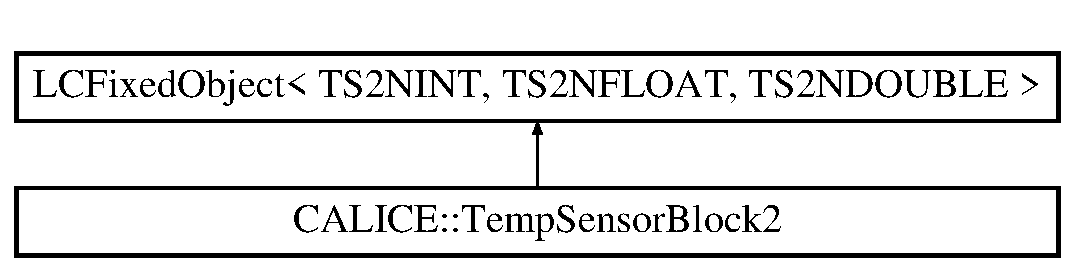
\includegraphics[height=2.000000cm]{classCALICE_1_1TempSensorBlock2}
\end{center}
\end{figure}
\subsection*{Public Member Functions}
\begin{DoxyCompactItemize}
\item 
{\bf Temp\-Sensor\-Block2} (int L\-D\-A\-Number, int Port\-Number, int T1, int T2, int T3, int T4, int T5, int T6, int T\-D\-I\-F, int T\-P\-W\-R)\label{classCALICE_1_1TempSensorBlock2_a54e191771f53ca8f7cbb1515d7aca02f}

\begin{DoxyCompactList}\small\item\em Convenient c'tor. \end{DoxyCompactList}\item 
{\bf Temp\-Sensor\-Block2} (L\-C\-Object $\ast$obj)\label{classCALICE_1_1TempSensorBlock2_a38018a53d6021897d93a8c5dceb4d414}

\begin{DoxyCompactList}\small\item\em 'Copy constructor' needed to interpret L\-C\-Collection read from file/database. \end{DoxyCompactList}\item 
virtual {\bf $\sim$\-Temp\-Sensor\-Block2} ()\label{classCALICE_1_1TempSensorBlock2_af5f34f2ff55c040772d6608011f215be}

\begin{DoxyCompactList}\small\item\em Important for memory handling. \end{DoxyCompactList}\item 
int {\bfseries Get\-L\-D\-A\-Number} () const \label{classCALICE_1_1TempSensorBlock2_a13a5db490dd71b4986d7f9a9f8305ed5}

\item 
int {\bfseries Get\-Port\-Number} () const \label{classCALICE_1_1TempSensorBlock2_ac954ae46175ebe0fc480e4961645149a}

\item 
int {\bfseries Get\-T1} () const \label{classCALICE_1_1TempSensorBlock2_aec4184305621faf41a9ad39a0b70eb34}

\item 
int {\bfseries Get\-T2} () const \label{classCALICE_1_1TempSensorBlock2_a910deb622a4882de3c245cdd74a792ed}

\item 
int {\bfseries Get\-T3} () const \label{classCALICE_1_1TempSensorBlock2_abec6d13fe16bb8e9afabbd7eabdc0dbc}

\item 
int {\bfseries Get\-T4} () const \label{classCALICE_1_1TempSensorBlock2_a8689abf3279957fe644cf450ee08ddc8}

\item 
int {\bfseries Get\-T5} () const \label{classCALICE_1_1TempSensorBlock2_a9f6702c33d6e3813b1d2b24b918d8d82}

\item 
int {\bfseries Get\-T6} () const \label{classCALICE_1_1TempSensorBlock2_a54d82a9b7521b8d9483ee600c1ad375f}

\item 
int {\bfseries Get\-T\-D\-I\-F} () const \label{classCALICE_1_1TempSensorBlock2_a833e1b88513124ae5370c2777dfa0bdd}

\item 
int {\bfseries Get\-T\-P\-W\-R} () const \label{classCALICE_1_1TempSensorBlock2_a9120824274d48a1a77218219de1139da}

\item 
void {\bfseries print} (std\-::ostream \&os, int)\label{classCALICE_1_1TempSensorBlock2_a18fcad9b01f87d568216df1198423cff}

\item 
const std\-::string {\bf get\-Type\-Name} () const \label{classCALICE_1_1TempSensorBlock2_aa7c390c29411439dbd83bd24f639570d}

\begin{DoxyCompactList}\small\item\em Return the type of the class. \end{DoxyCompactList}\item 
const std\-::string {\bf get\-Data\-Description} () const \label{classCALICE_1_1TempSensorBlock2_a876ddbe948463b85208e29cc03fc894b}

\begin{DoxyCompactList}\small\item\em Return a brief description of the data members. \end{DoxyCompactList}\end{DoxyCompactItemize}


\subsection{Detailed Description}
Class for the Labview Data as acquired by the A\-H\-C\-A\-L Labview. 

The class reflects that the data are received in the Labview \begin{DoxyAuthor}{Author}
S. Lu D\-E\-S\-Y Hamburg 
\end{DoxyAuthor}
\begin{DoxyDate}{Date}
Dec 17 2012 
\end{DoxyDate}


Definition at line 23 of file Temp\-Sensor\-Block2.\-hh.



The documentation for this class was generated from the following file\-:\begin{DoxyCompactItemize}
\item 
Temp\-Sensor\-Block2.\-hh\end{DoxyCompactItemize}

\section{C\-A\-L\-I\-C\-E\-:\-:Temp\-Sensor\-Block\-Old Class Reference}
\label{classCALICE_1_1TempSensorBlockOld}\index{C\-A\-L\-I\-C\-E\-::\-Temp\-Sensor\-Block\-Old@{C\-A\-L\-I\-C\-E\-::\-Temp\-Sensor\-Block\-Old}}


Class for the Labview Data as acquired by the A\-H\-C\-A\-L Labview.  




{\ttfamily \#include $<$Temp\-Sensor\-Block\-Old.\-hh$>$}

Inheritance diagram for C\-A\-L\-I\-C\-E\-:\-:Temp\-Sensor\-Block\-Old\-:\begin{figure}[H]
\begin{center}
\leavevmode
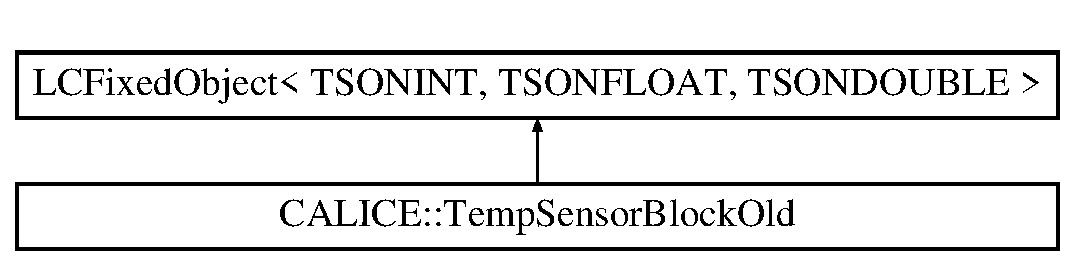
\includegraphics[height=2.000000cm]{classCALICE_1_1TempSensorBlockOld}
\end{center}
\end{figure}
\subsection*{Public Member Functions}
\begin{DoxyCompactItemize}
\item 
{\bf Temp\-Sensor\-Block\-Old} (float layer, float T1, float T2, float T3, float T4, float T5, float T6, float T\-D\-I\-F, float T\-P\-W\-R)\label{classCALICE_1_1TempSensorBlockOld_a82d44ba02d686f455a449b7973a84458}

\begin{DoxyCompactList}\small\item\em Convenient c'tor. \end{DoxyCompactList}\item 
{\bf Temp\-Sensor\-Block\-Old} (L\-C\-Object $\ast$obj)\label{classCALICE_1_1TempSensorBlockOld_a8fa3c63309c635a015babba9cd9bcc5e}

\begin{DoxyCompactList}\small\item\em 'Copy constructor' needed to interpret L\-C\-Collection read from file/database. \end{DoxyCompactList}\item 
virtual {\bf $\sim$\-Temp\-Sensor\-Block\-Old} ()\label{classCALICE_1_1TempSensorBlockOld_aa38e40270950ded8526b545854977c3c}

\begin{DoxyCompactList}\small\item\em Important for memory handling. \end{DoxyCompactList}\item 
float {\bfseries Get\-Layer} () const \label{classCALICE_1_1TempSensorBlockOld_ae6bf017ac104815ba921e869d089b995}

\item 
float {\bfseries Get\-T1} () const \label{classCALICE_1_1TempSensorBlockOld_a5a7ed17b117faae8ac76b9cc96e13296}

\item 
float {\bfseries Get\-T2} () const \label{classCALICE_1_1TempSensorBlockOld_a4663dda7309826ace2cf5bd61b67e5e0}

\item 
float {\bfseries Get\-T3} () const \label{classCALICE_1_1TempSensorBlockOld_af4a3ebf85837357ca3f779c4f76aec2a}

\item 
float {\bfseries Get\-T4} () const \label{classCALICE_1_1TempSensorBlockOld_a9d33ccb66b6ecc6fd9b09dc3ec74b05e}

\item 
float {\bfseries Get\-T5} () const \label{classCALICE_1_1TempSensorBlockOld_aa3e9bc414a3bb44caf97fcc815417790}

\item 
float {\bfseries Get\-T6} () const \label{classCALICE_1_1TempSensorBlockOld_af20c1b20fbd07c01f80ce2e9ad1ec03b}

\item 
float {\bfseries Get\-T\-D\-I\-F} () const \label{classCALICE_1_1TempSensorBlockOld_a5b6390ec23ce91e080f94188ecf2708f}

\item 
float {\bfseries Get\-T\-P\-W\-R} () const \label{classCALICE_1_1TempSensorBlockOld_a71713df3906fbd95f628d58d53c233f7}

\item 
void {\bfseries print} (std\-::ostream \&os, float)\label{classCALICE_1_1TempSensorBlockOld_afbe6d02c5fa6af5dedc8269ac47d3e53}

\item 
const std\-::string {\bf get\-Type\-Name} () const \label{classCALICE_1_1TempSensorBlockOld_aeeed0bef453e6e628add8cdc206febc0}

\begin{DoxyCompactList}\small\item\em Return the type of the class. \end{DoxyCompactList}\item 
const std\-::string {\bf get\-Data\-Description} () const \label{classCALICE_1_1TempSensorBlockOld_a1a0946cac03450c5f658780aee2c3ee6}

\begin{DoxyCompactList}\small\item\em Return a brief description of the data members. \end{DoxyCompactList}\end{DoxyCompactItemize}


\subsection{Detailed Description}
Class for the Labview Data as acquired by the A\-H\-C\-A\-L Labview. 

The class reflects that the data are received in the Labview \begin{DoxyAuthor}{Author}
S. Lu D\-E\-S\-Y Hamburg 
\end{DoxyAuthor}
\begin{DoxyDate}{Date}
Dec 17 2012 
\end{DoxyDate}


Definition at line 24 of file Temp\-Sensor\-Block\-Old.\-hh.



The documentation for this class was generated from the following file\-:\begin{DoxyCompactItemize}
\item 
Temp\-Sensor\-Block\-Old.\-hh\end{DoxyCompactItemize}

%--- End generated contents ---

% Index
\newpage
\phantomsection
\addcontentsline{toc}{part}{Index}
\printindex

\end{document}
